\PassOptionsToPackage{unicode=true}{hyperref} % options for packages loaded elsewhere
\PassOptionsToPackage{hyphens}{url}
%
\documentclass[]{article}
\usepackage{lmodern}
\usepackage{amssymb,amsmath}
\usepackage{ifxetex,ifluatex}
\usepackage{fixltx2e} % provides \textsubscript
\ifnum 0\ifxetex 1\fi\ifluatex 1\fi=0 % if pdftex
  \usepackage[T1]{fontenc}
  \usepackage[utf8]{inputenc}
  \usepackage{textcomp} % provides euro and other symbols
\else % if luatex or xelatex
  \usepackage{unicode-math}
  \defaultfontfeatures{Ligatures=TeX,Scale=MatchLowercase}
\fi
% use upquote if available, for straight quotes in verbatim environments
\IfFileExists{upquote.sty}{\usepackage{upquote}}{}
% use microtype if available
\IfFileExists{microtype.sty}{%
\usepackage[]{microtype}
\UseMicrotypeSet[protrusion]{basicmath} % disable protrusion for tt fonts
}{}
\IfFileExists{parskip.sty}{%
\usepackage{parskip}
}{% else
\setlength{\parindent}{0pt}
\setlength{\parskip}{6pt plus 2pt minus 1pt}
}
\usepackage{hyperref}
\hypersetup{
            pdftitle={Data Science R Basics},
            pdfborder={0 0 0},
            breaklinks=true}
\urlstyle{same}  % don't use monospace font for urls
\usepackage[margin=1in]{geometry}
\usepackage{color}
\usepackage{fancyvrb}
\newcommand{\VerbBar}{|}
\newcommand{\VERB}{\Verb[commandchars=\\\{\}]}
\DefineVerbatimEnvironment{Highlighting}{Verbatim}{commandchars=\\\{\}}
% Add ',fontsize=\small' for more characters per line
\usepackage{framed}
\definecolor{shadecolor}{RGB}{248,248,248}
\newenvironment{Shaded}{\begin{snugshade}}{\end{snugshade}}
\newcommand{\AlertTok}[1]{\textcolor[rgb]{0.94,0.16,0.16}{#1}}
\newcommand{\AnnotationTok}[1]{\textcolor[rgb]{0.56,0.35,0.01}{\textbf{\textit{#1}}}}
\newcommand{\AttributeTok}[1]{\textcolor[rgb]{0.77,0.63,0.00}{#1}}
\newcommand{\BaseNTok}[1]{\textcolor[rgb]{0.00,0.00,0.81}{#1}}
\newcommand{\BuiltInTok}[1]{#1}
\newcommand{\CharTok}[1]{\textcolor[rgb]{0.31,0.60,0.02}{#1}}
\newcommand{\CommentTok}[1]{\textcolor[rgb]{0.56,0.35,0.01}{\textit{#1}}}
\newcommand{\CommentVarTok}[1]{\textcolor[rgb]{0.56,0.35,0.01}{\textbf{\textit{#1}}}}
\newcommand{\ConstantTok}[1]{\textcolor[rgb]{0.00,0.00,0.00}{#1}}
\newcommand{\ControlFlowTok}[1]{\textcolor[rgb]{0.13,0.29,0.53}{\textbf{#1}}}
\newcommand{\DataTypeTok}[1]{\textcolor[rgb]{0.13,0.29,0.53}{#1}}
\newcommand{\DecValTok}[1]{\textcolor[rgb]{0.00,0.00,0.81}{#1}}
\newcommand{\DocumentationTok}[1]{\textcolor[rgb]{0.56,0.35,0.01}{\textbf{\textit{#1}}}}
\newcommand{\ErrorTok}[1]{\textcolor[rgb]{0.64,0.00,0.00}{\textbf{#1}}}
\newcommand{\ExtensionTok}[1]{#1}
\newcommand{\FloatTok}[1]{\textcolor[rgb]{0.00,0.00,0.81}{#1}}
\newcommand{\FunctionTok}[1]{\textcolor[rgb]{0.00,0.00,0.00}{#1}}
\newcommand{\ImportTok}[1]{#1}
\newcommand{\InformationTok}[1]{\textcolor[rgb]{0.56,0.35,0.01}{\textbf{\textit{#1}}}}
\newcommand{\KeywordTok}[1]{\textcolor[rgb]{0.13,0.29,0.53}{\textbf{#1}}}
\newcommand{\NormalTok}[1]{#1}
\newcommand{\OperatorTok}[1]{\textcolor[rgb]{0.81,0.36,0.00}{\textbf{#1}}}
\newcommand{\OtherTok}[1]{\textcolor[rgb]{0.56,0.35,0.01}{#1}}
\newcommand{\PreprocessorTok}[1]{\textcolor[rgb]{0.56,0.35,0.01}{\textit{#1}}}
\newcommand{\RegionMarkerTok}[1]{#1}
\newcommand{\SpecialCharTok}[1]{\textcolor[rgb]{0.00,0.00,0.00}{#1}}
\newcommand{\SpecialStringTok}[1]{\textcolor[rgb]{0.31,0.60,0.02}{#1}}
\newcommand{\StringTok}[1]{\textcolor[rgb]{0.31,0.60,0.02}{#1}}
\newcommand{\VariableTok}[1]{\textcolor[rgb]{0.00,0.00,0.00}{#1}}
\newcommand{\VerbatimStringTok}[1]{\textcolor[rgb]{0.31,0.60,0.02}{#1}}
\newcommand{\WarningTok}[1]{\textcolor[rgb]{0.56,0.35,0.01}{\textbf{\textit{#1}}}}
\usepackage{graphicx,grffile}
\makeatletter
\def\maxwidth{\ifdim\Gin@nat@width>\linewidth\linewidth\else\Gin@nat@width\fi}
\def\maxheight{\ifdim\Gin@nat@height>\textheight\textheight\else\Gin@nat@height\fi}
\makeatother
% Scale images if necessary, so that they will not overflow the page
% margins by default, and it is still possible to overwrite the defaults
% using explicit options in \includegraphics[width, height, ...]{}
\setkeys{Gin}{width=\maxwidth,height=\maxheight,keepaspectratio}
\setlength{\emergencystretch}{3em}  % prevent overfull lines
\providecommand{\tightlist}{%
  \setlength{\itemsep}{0pt}\setlength{\parskip}{0pt}}
\setcounter{secnumdepth}{0}
% Redefines (sub)paragraphs to behave more like sections
\ifx\paragraph\undefined\else
\let\oldparagraph\paragraph
\renewcommand{\paragraph}[1]{\oldparagraph{#1}\mbox{}}
\fi
\ifx\subparagraph\undefined\else
\let\oldsubparagraph\subparagraph
\renewcommand{\subparagraph}[1]{\oldsubparagraph{#1}\mbox{}}
\fi

% set default figure placement to htbp
\makeatletter
\def\fps@figure{htbp}
\makeatother


\title{Data Science R Basics}
\author{}
\date{\vspace{-2.5em}}

\begin{document}
\maketitle

\hypertarget{learning-objectives}{%
\subsection{Learning Objectives}\label{learning-objectives}}

\begin{itemize}
\tightlist
\item
  Learn to read, extract, and create datasets in R
\item
  Learn to perform a variety of operations on datasets using R
\item
  Learn to write your own functions/sub-routines in R
\end{itemize}

\hypertarget{course-overview}{%
\subsection{Course Overview}\label{course-overview}}

\hypertarget{section-1-r-basics-functions-data-types}{%
\subsubsection{Section 1: R Basics, Functions, Data
types}\label{section-1-r-basics-functions-data-types}}

You will get started with R, learn about its functions and data types.

\hypertarget{section-2-vectors-sorting}{%
\subsubsection{Section 2: Vectors,
Sorting}\label{section-2-vectors-sorting}}

You will learn to operate on vectors and advanced functions such as
sorting.

\hypertarget{section-3-indexing-data-manipulation-plots}{%
\subsubsection{Section 3: Indexing, Data Manipulation,
Plots}\label{section-3-indexing-data-manipulation-plots}}

You will learn to wrangle and visualize data.

\hypertarget{section-4-programming-basics}{%
\subsubsection{Section 4: Programming
Basics}\label{section-4-programming-basics}}

You will learn to use general programming features like `if-else', and
`for loop' commands, and write your own functions to perform various
operations on datasets.

\hypertarget{section-1-overview}{%
\subsection{Section 1 Overview}\label{section-1-overview}}

Section 1 introduces you to R Basics, Functions and Datatypes.

In Section 1, you will learn to:

\begin{itemize}
\tightlist
\item
  Appreciate the rationale for data analysis using R
\item
  Define objects and perform basic arithmetic and logical operations
\item
  Use pre-defined functions to perform operations on objects
\item
  Distinguish between various data types
\end{itemize}

The textbook for this section is available
\href{https://rafalab.github.io/dsbook/r-basics.html}{here}

\hypertarget{motivation}{%
\subsection{Motivation}\label{motivation}}

Here is a link to the
\href{https://rafalab.github.io/dsbook/r-basics.html\#case-study-us-gun-murders}{textbook
section on the motivation for this course}.

\hypertarget{getting-started}{%
\subsection{Getting started}\label{getting-started}}

Here is a link to the textbook section on
\href{https://rafalab.github.io/dsbook/getting-started.html}{Getting
Started} with R.

\textbf{Key Points}

\begin{itemize}
\tightlist
\item
  R was developed by statisticians and data analysts as an interactive
  environment for data analysis.
\item
  Some of the advantages of R are that (1) it is free and open source,
  (2) it has the capability to save scripts, (3) there are numerous
  resources for learning, and (4) it is easy for developers to share
  software implementation.
\item
  Expressions are evaluated in the R console when you type the
  expression into the console and hit Return.
\item
  A great advantage of R over point and click analysis software is that
  you can save your work as scripts.
\item
  ``Base R'' is what you get after you first install R. Additional
  components are available via packages.
\end{itemize}

\begin{Shaded}
\begin{Highlighting}[]
\CommentTok{# installing the dslabs package}
\ControlFlowTok{if}\NormalTok{(}\OperatorTok{!}\KeywordTok{require}\NormalTok{(dslabs)) }\KeywordTok{install.packages}\NormalTok{(}\StringTok{"dslabs"}\NormalTok{)}
\end{Highlighting}
\end{Shaded}

\begin{verbatim}
## Loading required package: dslabs
\end{verbatim}

\begin{Shaded}
\begin{Highlighting}[]
\CommentTok{# loading the dslabs package into the R session}
\KeywordTok{library}\NormalTok{(dslabs)}
\end{Highlighting}
\end{Shaded}

\hypertarget{installing-r-and-r-studio}{%
\subsection{Installing R and R Studio}\label{installing-r-and-r-studio}}

\hypertarget{installing-r}{%
\subsubsection{Installing R}\label{installing-r}}

To install R to work on your own computer, you can download it freely
from the \href{https://cran.r-project.org}{Comprehensive R Archive
Network} (CRAN). Note that CRAN makes several versions of R available:
versions for multiple operating systems and releases older than the
current one. You want to read the CRAN instructions to assure you
download the correct version. If you need further help, you read the
walkthrough in this
\href{https://rafalab.github.io/dsbook/installing-r-rstudio.html\#installing-r}{Chapter
of the textbook}.

\hypertarget{installing-rstudio}{%
\subsubsection{Installing RStudio}\label{installing-rstudio}}

RStudio is an integrated development environment (IDE). We highly
recommend installing and using RStudio to edit and test your code. You
can install RStudio through the
\href{https://rstudio.com/products/rstudio/download/}{RStudio website}.
Their
\href{https://rstudio.com/wp-content/uploads/2016/01/rstudio-IDE-cheatsheet.pdf}{cheatsheet}
is a great resource. You must install R before installing RStudio.

\hypertarget{textbook-link}{%
\subsubsection{Textbook Link}\label{textbook-link}}

Here is a link to the textbook section on
\href{https://rafalab.github.io/dsbook/installing-r-rstudio.html}{Installing
R and RStudio}.

\hypertarget{r-basics---objects}{%
\subsection{R Basics - Objects}\label{r-basics---objects}}

Here is a link to the textbook section on
\href{https://rafalab.github.io/dsbook/r-basics.html\#objects}{objects
in R}.

\textbf{Key Points}

\begin{itemize}
\tightlist
\item
  To define a variable, we may use the assignment symbol
  ``\textless{}-``.
\item
  There are two ways to see the value stored in a variable: (1) type the
  variable into the console and hit Return, or (2) type print(``variable
  name'') and hit Return.
\item
  Objects are stuff that is stored in R. They can be variables,
  functions, etc.
\item
  The ls() function shows the names of the objects saved in your
  workspace.
\end{itemize}

\emph{Solving the equation x2+x−1=0}

\begin{Shaded}
\begin{Highlighting}[]
\CommentTok{# assigning values to variables}
\NormalTok{a <-}\StringTok{ }\DecValTok{1}
\NormalTok{b <-}\StringTok{ }\DecValTok{1}
\NormalTok{c <-}\StringTok{ }\DecValTok{-1}

\CommentTok{# solving the quadratic equation}
\NormalTok{(}\OperatorTok{-}\NormalTok{b }\OperatorTok{+}\StringTok{ }\KeywordTok{sqrt}\NormalTok{(b}\OperatorTok{^}\DecValTok{2} \OperatorTok{-}\StringTok{ }\DecValTok{4}\OperatorTok{*}\NormalTok{a}\OperatorTok{*}\NormalTok{c) ) }\OperatorTok{/}\StringTok{ }\NormalTok{( }\DecValTok{2}\OperatorTok{*}\NormalTok{a )}
\end{Highlighting}
\end{Shaded}

\begin{verbatim}
## [1] 0.618034
\end{verbatim}

\begin{Shaded}
\begin{Highlighting}[]
\NormalTok{(}\OperatorTok{-}\NormalTok{b }\OperatorTok{-}\StringTok{ }\KeywordTok{sqrt}\NormalTok{(b}\OperatorTok{^}\DecValTok{2} \OperatorTok{-}\StringTok{ }\DecValTok{4}\OperatorTok{*}\NormalTok{a}\OperatorTok{*}\NormalTok{c) ) }\OperatorTok{/}\StringTok{ }\NormalTok{( }\DecValTok{2}\OperatorTok{*}\NormalTok{a )}
\end{Highlighting}
\end{Shaded}

\begin{verbatim}
## [1] -1.618034
\end{verbatim}

\hypertarget{r-basics---functions}{%
\subsection{R Basics - Functions}\label{r-basics---functions}}

Here is a link to the textbook section on
\href{https://rafalab.github.io/dsbook/r-basics.html\#functions}{functions}.

\textbf{Key points}

\begin{itemize}
\tightlist
\item
  In general, to evaluate a function we need to use parentheses. If we
  type a function without parenthesis, R shows us the code for the
  function. Most functions also require an argument, that is, something
  to be written inside the parenthesis.
\item
  To access help files, we may use the help function help(``function
  name''), or write the question mark followed by the function name.
\item
  The help file shows you the arguments the function is expecting, some
  of which are required and some are optional. If an argument is
  optional, a default value is assigned with the equal sign. The args()
  function also shows the arguments a function needs.
\item
  To specify arguments, we use the equals sign. If no argument name is
  used, R assumes you're entering arguments in the order shown in the
  help file.
\item
  Creating and saving a script makes code much easier to execute.
\item
  To make your code more readable, use intuitive variable names and
  include comments (using the ``\#'' symbol) to remind yourself why you
  wrote a particular line of code.
\end{itemize}

\hypertarget{assessment---r-basics}{%
\subsection{Assessment - R Basics}\label{assessment---r-basics}}

\begin{enumerate}
\def\labelenumi{\arabic{enumi}.}
\tightlist
\item
  What is the sum of the first n positive integers? We can use the
  formula \(n(n+1)/2\) to quickly compute this quantity.
\end{enumerate}

\begin{Shaded}
\begin{Highlighting}[]
\CommentTok{# Here is how you compute the sum for the first 20 integers}
\DecValTok{20}\OperatorTok{*}\NormalTok{(}\DecValTok{20}\OperatorTok{+}\DecValTok{1}\NormalTok{)}\OperatorTok{/}\DecValTok{2} 
\end{Highlighting}
\end{Shaded}

\begin{verbatim}
## [1] 210
\end{verbatim}

\begin{Shaded}
\begin{Highlighting}[]
\CommentTok{# However, we can define a variable to use the formula for other values of n}
\NormalTok{n <-}\StringTok{ }\DecValTok{20}
\NormalTok{n}\OperatorTok{*}\NormalTok{(n}\OperatorTok{+}\DecValTok{1}\NormalTok{)}\OperatorTok{/}\DecValTok{2}
\end{Highlighting}
\end{Shaded}

\begin{verbatim}
## [1] 210
\end{verbatim}

\begin{Shaded}
\begin{Highlighting}[]
\NormalTok{n <-}\StringTok{ }\DecValTok{25}
\NormalTok{n}\OperatorTok{*}\NormalTok{(n}\OperatorTok{+}\DecValTok{1}\NormalTok{)}\OperatorTok{/}\DecValTok{2}
\end{Highlighting}
\end{Shaded}

\begin{verbatim}
## [1] 325
\end{verbatim}

\begin{Shaded}
\begin{Highlighting}[]
\CommentTok{# Below, write code to calculate the sum of the first 100 integers}
\NormalTok{n<-}\DecValTok{100}
\NormalTok{n}\OperatorTok{*}\NormalTok{(n}\OperatorTok{+}\DecValTok{1}\NormalTok{)}\OperatorTok{/}\DecValTok{2}
\end{Highlighting}
\end{Shaded}

\begin{verbatim}
## [1] 5050
\end{verbatim}

\begin{enumerate}
\def\labelenumi{\arabic{enumi}.}
\setcounter{enumi}{1}
\tightlist
\item
  What is the sum of the first 1000 positive integers? We can use the
  formula \(n(n+1)/2\) to quickly compute this quantity.
\end{enumerate}

\begin{Shaded}
\begin{Highlighting}[]
\CommentTok{# Below, write code to calculate the sum of the first 1000 integers }
\NormalTok{n<-}\DecValTok{1000}
\NormalTok{n}\OperatorTok{*}\NormalTok{(n}\OperatorTok{+}\DecValTok{1}\NormalTok{)}\OperatorTok{/}\DecValTok{2}
\end{Highlighting}
\end{Shaded}

\begin{verbatim}
## [1] 500500
\end{verbatim}

\begin{enumerate}
\def\labelenumi{\arabic{enumi}.}
\setcounter{enumi}{2}
\tightlist
\item
  Run the following code in the R console.
\end{enumerate}

\begin{Shaded}
\begin{Highlighting}[]
\NormalTok{n <-}\StringTok{ }\DecValTok{1000}
\NormalTok{x <-}\StringTok{ }\KeywordTok{seq}\NormalTok{(}\DecValTok{1}\NormalTok{, n)}
\KeywordTok{sum}\NormalTok{(x)}
\end{Highlighting}
\end{Shaded}

\begin{verbatim}
## [1] 500500
\end{verbatim}

Based on the result, what do you think the functions \texttt{seq} and
\texttt{sum} do?

\begin{itemize}
\tightlist
\item
  {[} {]} A. sum creates a list of numbers and seq adds them up.
\item
  {[}X{]} B. seq creates a list of numbers and sum adds them up.
\item
  {[} {]} C. seq computes the difference between two arguments and sum
  computes the sum of 1 through 1000.
\item
  {[} {]} D. sum always returns the same number.
\end{itemize}

\begin{enumerate}
\def\labelenumi{\arabic{enumi}.}
\setcounter{enumi}{3}
\tightlist
\item
  In math and programming we say we evaluate a function when we replace
  arguments with specific values. So if we type \texttt{log2(16)} we
  evaluate the \texttt{log2} function to get the log base 2 of
  \texttt{16} which is \texttt{4}.
\end{enumerate}

In R it is often useful to evaluate a function inside another function.
For example, \texttt{sqrt(log2(16))} will calculate the log to the base
2 of 16 and then compute the square root of that value. So the first
evaluation gives a 4 and this gets evaluated by \texttt{sqrt} to give
the final answer of 2.

\begin{Shaded}
\begin{Highlighting}[]
\CommentTok{# log to the base 2 }
\KeywordTok{log2}\NormalTok{(}\DecValTok{16}\NormalTok{)}
\end{Highlighting}
\end{Shaded}

\begin{verbatim}
## [1] 4
\end{verbatim}

\begin{Shaded}
\begin{Highlighting}[]
\CommentTok{# sqrt of the log to the base 2 of 16:}
\KeywordTok{sqrt}\NormalTok{(}\KeywordTok{log2}\NormalTok{(}\DecValTok{16}\NormalTok{))}
\end{Highlighting}
\end{Shaded}

\begin{verbatim}
## [1] 2
\end{verbatim}

\begin{Shaded}
\begin{Highlighting}[]
\CommentTok{# Compute log to the base 10 (log10) of the sqrt of 100. Do not use variables.}
\KeywordTok{log10}\NormalTok{(}\KeywordTok{sqrt}\NormalTok{(}\DecValTok{100}\NormalTok{))}
\end{Highlighting}
\end{Shaded}

\begin{verbatim}
## [1] 1
\end{verbatim}

\begin{enumerate}
\def\labelenumi{\arabic{enumi}.}
\setcounter{enumi}{4}
\tightlist
\item
  Which of the following will always return the numeric value stored in
  \texttt{x}? You can try out examples and use the help system in the R
  console.
\end{enumerate}

\begin{itemize}
\tightlist
\item
  {[} {]} A. log(10\^{}x)
\item
  {[} {]} B. log10(x\^{}10)
\item
  {[}X{]} C. log(exp(x))
\item
  {[} {]} D. exp(log(x, base = 2))
\end{itemize}

\hypertarget{data-types}{%
\subsection{Data Types}\label{data-types}}

You can find the
\href{https://rafalab.github.io/dsbook/r-basics.html\#data-types}{section
of the textbook on data types here}.

\textbf{Key Points}

\begin{itemize}
\tightlist
\item
  The function ``class'' helps us determine the type of an object.
\item
  Data frames can be thought of as tables with rows representing
  observations and columns representing different variables.
\item
  To access data from columns of a data frame, we use the dollar sign
  symbol, which is called the accessor.
\item
  A vector is an object consisting of several entries and can be a
  numeric vector, a character vector, or a logical vector.
\item
  We use quotes to distinguish between variable names and character
  strings.
\item
  Factors are useful for storing categorical data, and are more memory
  efficient than storing characters.
\end{itemize}

\emph{Code}

\begin{Shaded}
\begin{Highlighting}[]
\CommentTok{# loading the the murders dataset}
\KeywordTok{data}\NormalTok{(murders)}

\CommentTok{# determining that the murders dataset is of the "data frame" class}
\KeywordTok{class}\NormalTok{(murders)}
\end{Highlighting}
\end{Shaded}

\begin{verbatim}
## [1] "data.frame"
\end{verbatim}

\begin{Shaded}
\begin{Highlighting}[]
\CommentTok{# finding out more about the structure of the object}
\KeywordTok{str}\NormalTok{(murders)}
\end{Highlighting}
\end{Shaded}

\begin{verbatim}
## 'data.frame':    51 obs. of  5 variables:
##  $ state     : chr  "Alabama" "Alaska" "Arizona" "Arkansas" ...
##  $ abb       : chr  "AL" "AK" "AZ" "AR" ...
##  $ region    : Factor w/ 4 levels "Northeast","South",..: 2 4 4 2 4 4 1 2 2 2 ...
##  $ population: num  4779736 710231 6392017 2915918 37253956 ...
##  $ total     : num  135 19 232 93 1257 ...
\end{verbatim}

\begin{Shaded}
\begin{Highlighting}[]
\CommentTok{# showing the first 6 lines of the dataset}
\KeywordTok{head}\NormalTok{(murders)}
\end{Highlighting}
\end{Shaded}

\begin{verbatim}
##        state abb region population total
## 1    Alabama  AL  South    4779736   135
## 2     Alaska  AK   West     710231    19
## 3    Arizona  AZ   West    6392017   232
## 4   Arkansas  AR  South    2915918    93
## 5 California  CA   West   37253956  1257
## 6   Colorado  CO   West    5029196    65
\end{verbatim}

\begin{Shaded}
\begin{Highlighting}[]
\CommentTok{# using the accessor operator to obtain the population column}
\NormalTok{murders}\OperatorTok{$}\NormalTok{population}
\end{Highlighting}
\end{Shaded}

\begin{verbatim}
##  [1]  4779736   710231  6392017  2915918 37253956  5029196  3574097   897934
##  [9]   601723 19687653  9920000  1360301  1567582 12830632  6483802  3046355
## [17]  2853118  4339367  4533372  1328361  5773552  6547629  9883640  5303925
## [25]  2967297  5988927   989415  1826341  2700551  1316470  8791894  2059179
## [33] 19378102  9535483   672591 11536504  3751351  3831074 12702379  1052567
## [41]  4625364   814180  6346105 25145561  2763885   625741  8001024  6724540
## [49]  1852994  5686986   563626
\end{verbatim}

\begin{Shaded}
\begin{Highlighting}[]
\CommentTok{# displaying the variable names in the murders dataset}
\KeywordTok{names}\NormalTok{(murders)}
\end{Highlighting}
\end{Shaded}

\begin{verbatim}
## [1] "state"      "abb"        "region"     "population" "total"
\end{verbatim}

\begin{Shaded}
\begin{Highlighting}[]
\CommentTok{# determining how many entries are in a vector}
\NormalTok{pop <-}\StringTok{ }\NormalTok{murders}\OperatorTok{$}\NormalTok{population}
\KeywordTok{length}\NormalTok{(pop)}
\end{Highlighting}
\end{Shaded}

\begin{verbatim}
## [1] 51
\end{verbatim}

\begin{Shaded}
\begin{Highlighting}[]
\CommentTok{# vectors can be of class numeric and character}
\KeywordTok{class}\NormalTok{(pop)}
\end{Highlighting}
\end{Shaded}

\begin{verbatim}
## [1] "numeric"
\end{verbatim}

\begin{Shaded}
\begin{Highlighting}[]
\KeywordTok{class}\NormalTok{(murders}\OperatorTok{$}\NormalTok{state)}
\end{Highlighting}
\end{Shaded}

\begin{verbatim}
## [1] "character"
\end{verbatim}

\begin{Shaded}
\begin{Highlighting}[]
\CommentTok{# logical vectors are either TRUE or FALSE}
\NormalTok{z <-}\StringTok{ }\DecValTok{3} \OperatorTok{==}\StringTok{ }\DecValTok{2}
\NormalTok{z}
\end{Highlighting}
\end{Shaded}

\begin{verbatim}
## [1] FALSE
\end{verbatim}

\begin{Shaded}
\begin{Highlighting}[]
\KeywordTok{class}\NormalTok{(z)}
\end{Highlighting}
\end{Shaded}

\begin{verbatim}
## [1] "logical"
\end{verbatim}

\begin{Shaded}
\begin{Highlighting}[]
\CommentTok{# factors are another type of class}
\KeywordTok{class}\NormalTok{(murders}\OperatorTok{$}\NormalTok{region)}
\end{Highlighting}
\end{Shaded}

\begin{verbatim}
## [1] "factor"
\end{verbatim}

\begin{Shaded}
\begin{Highlighting}[]
\CommentTok{# obtaining the levels of a factor}
\KeywordTok{levels}\NormalTok{(murders}\OperatorTok{$}\NormalTok{region)}
\end{Highlighting}
\end{Shaded}

\begin{verbatim}
## [1] "Northeast"     "South"         "North Central" "West"
\end{verbatim}

\hypertarget{assessment---data-types}{%
\subsection{Assessment - Data Types}\label{assessment---data-types}}

\begin{enumerate}
\def\labelenumi{\arabic{enumi}.}
\tightlist
\item
  We're going to be using the following dataset for this module. Run
  this code in the console.
\end{enumerate}

\begin{Shaded}
\begin{Highlighting}[]
\KeywordTok{library}\NormalTok{(dslabs)  }
\KeywordTok{data}\NormalTok{(murders)}
\end{Highlighting}
\end{Shaded}

Next, use the function \texttt{str} to examine the structure of the
\texttt{murders} object. We can see that this object is a data frame
with 51 rows and five columns.

\begin{Shaded}
\begin{Highlighting}[]
\KeywordTok{str}\NormalTok{(murders)}
\end{Highlighting}
\end{Shaded}

\begin{verbatim}
## 'data.frame':    51 obs. of  5 variables:
##  $ state     : chr  "Alabama" "Alaska" "Arizona" "Arkansas" ...
##  $ abb       : chr  "AL" "AK" "AZ" "AR" ...
##  $ region    : Factor w/ 4 levels "Northeast","South",..: 2 4 4 2 4 4 1 2 2 2 ...
##  $ population: num  4779736 710231 6392017 2915918 37253956 ...
##  $ total     : num  135 19 232 93 1257 ...
\end{verbatim}

Which of the following best describes the variables represented in this
data frame?

\begin{itemize}
\tightlist
\item
  {[} {]} A. The 51 states.
\item
  {[} {]} B. The murder rates for all 50 states and DC.
\item
  {[}X{]} C. The state name, the abbreviation of the state name, the
  state's region, and the state's population and total number of murders
  for 2010.
\item
  {[} {]} D. str shows no relevant information.
\end{itemize}

\begin{enumerate}
\def\labelenumi{\arabic{enumi}.}
\setcounter{enumi}{1}
\tightlist
\item
  In the previous question, we saw the different variables that are a
  part of this dataset from the output of the \texttt{str()} function.
  The function \texttt{names()} is specifically designed to extract the
  column names from a data frame.
\end{enumerate}

\begin{Shaded}
\begin{Highlighting}[]
\CommentTok{# Load package and data}
\KeywordTok{library}\NormalTok{(dslabs)}
\KeywordTok{data}\NormalTok{(murders)}
\end{Highlighting}
\end{Shaded}

\begin{Shaded}
\begin{Highlighting}[]
\CommentTok{# Use the function names to extract the variable names }
\KeywordTok{names}\NormalTok{(murders)}
\end{Highlighting}
\end{Shaded}

\begin{verbatim}
## [1] "state"      "abb"        "region"     "population" "total"
\end{verbatim}

\begin{enumerate}
\def\labelenumi{\arabic{enumi}.}
\setcounter{enumi}{2}
\tightlist
\item
  In this module we have learned that every variable has a class. For
  example, the class can be a \emph{character}, \emph{numeric} or
  \emph{logical}. The function \texttt{class()} can be used to determine
  the class of an object.
\end{enumerate}

Here we are going to determine the class of one of the variables in the
\texttt{murders} data frame. To extract variables from a data frame we
use \texttt{\$}, referred to as the accessor.

\begin{Shaded}
\begin{Highlighting}[]
\CommentTok{# To access the population variable from the murders dataset use this code:}
\NormalTok{p <-}\StringTok{ }\NormalTok{murders}\OperatorTok{$}\NormalTok{population }

\CommentTok{# To determine the class of object `p` we use this code:}
\KeywordTok{class}\NormalTok{(p)}
\end{Highlighting}
\end{Shaded}

\begin{verbatim}
## [1] "numeric"
\end{verbatim}

\begin{Shaded}
\begin{Highlighting}[]
\CommentTok{# Use the accessor to extract state abbreviations and assign it to a}
\NormalTok{a <-}\StringTok{ }\NormalTok{murders}\OperatorTok{$}\NormalTok{abb}

\CommentTok{# Determine the class of a}
\KeywordTok{class}\NormalTok{(a)}
\end{Highlighting}
\end{Shaded}

\begin{verbatim}
## [1] "character"
\end{verbatim}

\begin{enumerate}
\def\labelenumi{\arabic{enumi}.}
\setcounter{enumi}{3}
\tightlist
\item
  An important lesson you should learn early on is that there are
  multiple ways to do things in R. For example, to generate the first
  five integers we note that \texttt{1:5} and \texttt{seq(1,5)} return
  the same result.
\end{enumerate}

There are also multiple ways to access variables in a data frame. For
example we can use the square brackets \texttt{{[}{[}} instead of the
accessor \texttt{\$}.

If you instead try to access a column with just one bracket,

\begin{Shaded}
\begin{Highlighting}[]
\NormalTok{murders[}\StringTok{"population"}\NormalTok{]}
\end{Highlighting}
\end{Shaded}

R returns a subset of the original data frame containing just this
column. This new object will be of class \texttt{data.frame} rather than
a vector. To access the column itself you need to use either the
\texttt{\$} accessor or the double square brackets \texttt{{[}{[}}.

Parentheses, in contrast, are mainly used alongside functions to
indicate what argument the function should be doing something to. For
example, when we did \texttt{class(p)} in the last question, we wanted
the function \texttt{class} to do something related to the argument
\texttt{p}.

This is an example of how R can be a bit idiosyncratic sometimes. It is
very common to find it confusing at first.

\begin{Shaded}
\begin{Highlighting}[]
\CommentTok{# We extract the population like this:}
\NormalTok{p <-}\StringTok{ }\NormalTok{murders}\OperatorTok{$}\NormalTok{population}

\CommentTok{# This is how we do the same with the square brackets:}
\NormalTok{o <-}\StringTok{ }\NormalTok{murders[[}\StringTok{"population"}\NormalTok{]]}

\CommentTok{# We can confirm these two are the same}
\KeywordTok{identical}\NormalTok{(o, p)}
\end{Highlighting}
\end{Shaded}

\begin{verbatim}
## [1] TRUE
\end{verbatim}

\begin{Shaded}
\begin{Highlighting}[]
\CommentTok{# Use square brackets to extract `abb` from `murders` and assign it to b}
\NormalTok{b <-}\StringTok{ }\NormalTok{murders[[}\StringTok{"abb"}\NormalTok{]]}

\CommentTok{# Check if `a` and `b` are identical }
\KeywordTok{identical}\NormalTok{(a, b)}
\end{Highlighting}
\end{Shaded}

\begin{verbatim}
## [1] TRUE
\end{verbatim}

\begin{enumerate}
\def\labelenumi{\arabic{enumi}.}
\setcounter{enumi}{4}
\tightlist
\item
  Using the \texttt{str()} command, we saw that the \emph{region} column
  stores a factor. You can corroborate this by using the \texttt{class}
  command on the \emph{region} column.
\end{enumerate}

The function \texttt{levels} shows us the categories for the factor.

\begin{Shaded}
\begin{Highlighting}[]
\CommentTok{# We can see the class of the region variable using class}
\KeywordTok{class}\NormalTok{(murders}\OperatorTok{$}\NormalTok{region)}
\end{Highlighting}
\end{Shaded}

\begin{verbatim}
## [1] "factor"
\end{verbatim}

\begin{Shaded}
\begin{Highlighting}[]
\CommentTok{# Determine the number of regions included in this variable }
\KeywordTok{length}\NormalTok{(}\KeywordTok{levels}\NormalTok{(murders}\OperatorTok{$}\NormalTok{region))}
\end{Highlighting}
\end{Shaded}

\begin{verbatim}
## [1] 4
\end{verbatim}

\begin{enumerate}
\def\labelenumi{\arabic{enumi}.}
\setcounter{enumi}{5}
\tightlist
\item
  The function \texttt{table} takes a vector as input and returns the
  frequency of each unique element in the vector.
\end{enumerate}

\begin{Shaded}
\begin{Highlighting}[]
\CommentTok{# Here is an example of what the table function does}
\NormalTok{x <-}\StringTok{ }\KeywordTok{c}\NormalTok{(}\StringTok{"a"}\NormalTok{, }\StringTok{"a"}\NormalTok{, }\StringTok{"b"}\NormalTok{, }\StringTok{"b"}\NormalTok{, }\StringTok{"b"}\NormalTok{, }\StringTok{"c"}\NormalTok{)}
\KeywordTok{table}\NormalTok{(x)}
\end{Highlighting}
\end{Shaded}

\begin{verbatim}
## x
## a b c 
## 2 3 1
\end{verbatim}

\begin{Shaded}
\begin{Highlighting}[]
\CommentTok{# Write one line of code to show the number of states per region}
\KeywordTok{table}\NormalTok{(murders}\OperatorTok{$}\NormalTok{region)}
\end{Highlighting}
\end{Shaded}

\begin{verbatim}
## 
##     Northeast         South North Central          West 
##             9            17            12            13
\end{verbatim}

\hypertarget{section-1-assessment}{%
\subsection{Section 1 Assessment}\label{section-1-assessment}}

\begin{enumerate}
\def\labelenumi{\arabic{enumi}.}
\tightlist
\item
  To find the solutions to an equation of the format \(ax^2+bx+c\), use
  the quadratic equation: \(x=\frac{-b±\sqrt(b^2−4ac)}{2a}\).
\end{enumerate}

What are the two solutions to \(2x^2-x-4=0\)? Use the quadratic
equation. (Report the greater of the two solutions first, using 3
significant digits for both solutions)

\begin{Shaded}
\begin{Highlighting}[]
\KeywordTok{options}\NormalTok{(}\DataTypeTok{digits =} \DecValTok{3}\NormalTok{)}
\NormalTok{a <-}\StringTok{ }\DecValTok{2}
\NormalTok{b <-}\StringTok{ }\DecValTok{-1}
\NormalTok{c <-}\StringTok{ }\DecValTok{-4}
\NormalTok{(}\OperatorTok{-}\NormalTok{b}\OperatorTok{+}\KeywordTok{sqrt}\NormalTok{(b}\OperatorTok{^}\DecValTok{2-4}\OperatorTok{*}\NormalTok{a}\OperatorTok{*}\NormalTok{c))}\OperatorTok{/}\NormalTok{(}\DecValTok{2}\OperatorTok{*}\NormalTok{a)}
\end{Highlighting}
\end{Shaded}

\begin{verbatim}
## [1] 1.69
\end{verbatim}

\begin{Shaded}
\begin{Highlighting}[]
\NormalTok{(}\OperatorTok{-}\NormalTok{b}\OperatorTok{-}\KeywordTok{sqrt}\NormalTok{(b}\OperatorTok{^}\DecValTok{2-4}\OperatorTok{*}\NormalTok{a}\OperatorTok{*}\NormalTok{c))}\OperatorTok{/}\NormalTok{(}\DecValTok{2}\OperatorTok{*}\NormalTok{a)}
\end{Highlighting}
\end{Shaded}

\begin{verbatim}
## [1] -1.19
\end{verbatim}

\begin{enumerate}
\def\labelenumi{\arabic{enumi}.}
\setcounter{enumi}{1}
\tightlist
\item
  Use R to compute log base 4 of 1024. You can use the \texttt{help}
  function to learn how to use arguments to change the base of the
  \texttt{log} function.
\end{enumerate}

\begin{Shaded}
\begin{Highlighting}[]
\KeywordTok{log}\NormalTok{(}\DecValTok{1024}\NormalTok{, }\DataTypeTok{base =} \DecValTok{4}\NormalTok{)}
\end{Highlighting}
\end{Shaded}

\begin{verbatim}
## [1] 5
\end{verbatim}

\begin{enumerate}
\def\labelenumi{\arabic{enumi}.}
\setcounter{enumi}{2}
\tightlist
\item
  Load the \texttt{movielens} dataset
\end{enumerate}

\begin{Shaded}
\begin{Highlighting}[]
\KeywordTok{data}\NormalTok{(movielens)}
\KeywordTok{str}\NormalTok{(movielens)}
\end{Highlighting}
\end{Shaded}

\begin{verbatim}
## 'data.frame':    100004 obs. of  7 variables:
##  $ movieId  : int  31 1029 1061 1129 1172 1263 1287 1293 1339 1343 ...
##  $ title    : chr  "Dangerous Minds" "Dumbo" "Sleepers" "Escape from New York" ...
##  $ year     : int  1995 1941 1996 1981 1989 1978 1959 1982 1992 1991 ...
##  $ genres   : Factor w/ 901 levels "(no genres listed)",..: 762 510 899 120 762 836 81 762 844 899 ...
##  $ userId   : int  1 1 1 1 1 1 1 1 1 1 ...
##  $ rating   : num  2.5 3 3 2 4 2 2 2 3.5 2 ...
##  $ timestamp: int  1260759144 1260759179 1260759182 1260759185 1260759205 1260759151 1260759187 1260759148 1260759125 1260759131 ...
\end{verbatim}

How many rows are in the dataset? \texttt{100004}

How many different variables are in the dataset? \texttt{7}

What is the variable type of \texttt{title}?

\begin{itemize}
\tightlist
\item
  {[} {]} A. It is a text (txt) variable
\item
  {[} {]} B. It is a chronological (chr) variable
\item
  {[} {]} C. It is a string (str) variable
\item
  {[} {]} D. It is a numeric (num) variable
\item
  {[} {]} E. It is an integer (int) variable
\item
  {[} {]} F. It is a factor (Factor) variable
\item
  {[}X{]} G. It is a character (chr) variable
\end{itemize}

What is the variable type of \texttt{genres}?

\begin{itemize}
\tightlist
\item
  {[} {]} A. It is a text (txt) variable
\item
  {[} {]} B. It is a chronological (chr) variable
\item
  {[} {]} C. It is a string (str) variable
\item
  {[} {]} D. It is a numeric (num) variable
\item
  {[} {]} E. It is an integer (int) variable
\item
  {[}X{]} F. It is a factor (Factor) variable
\item
  {[} {]} G. It is a character (chr) variable
\end{itemize}

\begin{enumerate}
\def\labelenumi{\arabic{enumi}.}
\setcounter{enumi}{3}
\tightlist
\item
  We already know we can use the \texttt{levels()} function to determine
  the levels of a factor. A different function, \texttt{nlevels()}, may
  be used to determine the number of levels of a factor.
\end{enumerate}

Use this function to determine how many levels are in the factor
\texttt{genres} in the \texttt{movielens} data frame.

\begin{Shaded}
\begin{Highlighting}[]
\KeywordTok{nlevels}\NormalTok{(movielens}\OperatorTok{$}\NormalTok{genres)}
\end{Highlighting}
\end{Shaded}

\begin{verbatim}
## [1] 901
\end{verbatim}

\hypertarget{section-2-overview}{%
\subsection{Section 2 Overview}\label{section-2-overview}}

In Section 2.1, you will:

\begin{itemize}
\tightlist
\item
  Create numeric and character vectors.
\item
  Name the columns of a vector.
\item
  Generate numeric sequences.
\item
  Access specific elements or parts of a vector.
\item
  Coerce data into different data types as needed.
\end{itemize}

In Section 2.2, you will:

\begin{itemize}
\tightlist
\item
  Sort vectors in ascending and descending order.
\item
  Extract the indices of the sorted elements from the original vector.
\item
  Find the maximum and minimum elements, as well as their indices, in a
  vector.
\item
  Rank the elements of a vector in increasing order.
\end{itemize}

In Section 2.3, you will:

\begin{itemize}
\tightlist
\item
  Perform arithmetic between a vector and a single number.
\item
  Perform arithmetic between two vectors of same length.
\end{itemize}

\hypertarget{vectors}{%
\subsection{Vectors}\label{vectors}}

The textbook for this section is available
\href{https://rafalab.github.io/dsbook/r-basics.html\#vectors}{here}

\textbf{Key Points}

\begin{itemize}
\tightlist
\item
  The function \texttt{c()}, which stands for concatenate, is useful for
  creating vectors.
\item
  Another useful function for creating vectors is the \texttt{seq()}
  function, which generates sequences.
\item
  Subsetting lets us access specific parts of a vector by using square
  brackets to access elements of a vector.
\end{itemize}

\emph{Code}

\begin{Shaded}
\begin{Highlighting}[]
\CommentTok{# We may create vectors of class numeric or character with the concatenate function}
\NormalTok{codes <-}\StringTok{ }\KeywordTok{c}\NormalTok{(}\DecValTok{380}\NormalTok{, }\DecValTok{124}\NormalTok{, }\DecValTok{818}\NormalTok{)}
\NormalTok{country <-}\StringTok{ }\KeywordTok{c}\NormalTok{(}\StringTok{"italy"}\NormalTok{, }\StringTok{"canada"}\NormalTok{, }\StringTok{"egypt"}\NormalTok{)}

\CommentTok{# We can also name the elements of a numeric vector}
\CommentTok{# Note that the two lines of code below have the same result}
\NormalTok{codes <-}\StringTok{ }\KeywordTok{c}\NormalTok{(}\DataTypeTok{italy =} \DecValTok{380}\NormalTok{, }\DataTypeTok{canada =} \DecValTok{124}\NormalTok{, }\DataTypeTok{egypt =} \DecValTok{818}\NormalTok{)}
\NormalTok{codes <-}\StringTok{ }\KeywordTok{c}\NormalTok{(}\StringTok{"italy"}\NormalTok{ =}\StringTok{ }\DecValTok{380}\NormalTok{, }\StringTok{"canada"}\NormalTok{ =}\StringTok{ }\DecValTok{124}\NormalTok{, }\StringTok{"egypt"}\NormalTok{ =}\StringTok{ }\DecValTok{818}\NormalTok{)}

\CommentTok{# We can also name the elements of a numeric vector using the names() function}
\NormalTok{codes <-}\StringTok{ }\KeywordTok{c}\NormalTok{(}\DecValTok{380}\NormalTok{, }\DecValTok{124}\NormalTok{, }\DecValTok{818}\NormalTok{)}
\NormalTok{country <-}\StringTok{ }\KeywordTok{c}\NormalTok{(}\StringTok{"italy"}\NormalTok{,}\StringTok{"canada"}\NormalTok{,}\StringTok{"egypt"}\NormalTok{)}
\KeywordTok{names}\NormalTok{(codes) <-}\StringTok{ }\NormalTok{country}

\CommentTok{# Using square brackets is useful for subsetting to access specific elements of a vector}
\NormalTok{codes[}\DecValTok{2}\NormalTok{]}
\end{Highlighting}
\end{Shaded}

\begin{verbatim}
## canada 
##    124
\end{verbatim}

\begin{Shaded}
\begin{Highlighting}[]
\NormalTok{codes[}\KeywordTok{c}\NormalTok{(}\DecValTok{1}\NormalTok{,}\DecValTok{3}\NormalTok{)]}
\end{Highlighting}
\end{Shaded}

\begin{verbatim}
## italy egypt 
##   380   818
\end{verbatim}

\begin{Shaded}
\begin{Highlighting}[]
\NormalTok{codes[}\DecValTok{1}\OperatorTok{:}\DecValTok{2}\NormalTok{]}
\end{Highlighting}
\end{Shaded}

\begin{verbatim}
##  italy canada 
##    380    124
\end{verbatim}

\begin{Shaded}
\begin{Highlighting}[]
\CommentTok{# If the entries of a vector are named, they may be accessed by referring to their name}
\NormalTok{codes[}\StringTok{"canada"}\NormalTok{]}
\end{Highlighting}
\end{Shaded}

\begin{verbatim}
## canada 
##    124
\end{verbatim}

\begin{Shaded}
\begin{Highlighting}[]
\NormalTok{codes[}\KeywordTok{c}\NormalTok{(}\StringTok{"egypt"}\NormalTok{,}\StringTok{"italy"}\NormalTok{)]}
\end{Highlighting}
\end{Shaded}

\begin{verbatim}
## egypt italy 
##   818   380
\end{verbatim}

\hypertarget{vectors---vector-coercion}{%
\subsection{Vectors - Vector Coercion}\label{vectors---vector-coercion}}

The textbook for this section is available
\href{https://rafalab.github.io/dsbook/r-basics.html\#coercion}{here}

\textbf{Key Points}

\begin{itemize}
\tightlist
\item
  In general, \emph{coercion} is an attempt by R to be flexible with
  data types by guessing what was meant when an entry does not match the
  expected. For example, when defining x as
\end{itemize}

x \textless{}- c(1, ``canada'', 3)

R \emph{coerced} the data into characters. It guessed that because you
put a character string in the vector, you meant the 1 and 3 to actually
be character strings ``1'' and ``3''.

\begin{itemize}
\tightlist
\item
  The function \texttt{as.character()} turns numbers into characters.
\item
  The function \texttt{as.numeric()} turns characters into numbers.
\item
  In R, missing data is assigned the value NA.
\end{itemize}

\hypertarget{assessment---vectors}{%
\subsection{Assessment - Vectors}\label{assessment---vectors}}

\begin{enumerate}
\def\labelenumi{\arabic{enumi}.}
\tightlist
\item
  A vector is a series of values, all of the same type. They are the
  most basic data type in R and can hold numeric data, character data,
  or logical data. In R, you can create a vector with the concatenate
  (or combine) function \texttt{c()}
\end{enumerate}

You place the vector elements separated by a comma between the
parentheses. For example a numeric vector would look something like
this:

\begin{Shaded}
\begin{Highlighting}[]
\NormalTok{cost <-}\StringTok{ }\KeywordTok{c}\NormalTok{(}\DecValTok{50}\NormalTok{, }\DecValTok{75}\NormalTok{, }\DecValTok{90}\NormalTok{, }\DecValTok{100}\NormalTok{, }\DecValTok{150}\NormalTok{)}
\end{Highlighting}
\end{Shaded}

\begin{Shaded}
\begin{Highlighting}[]
\CommentTok{# Here is an example creating a numeric vector named cost}
\NormalTok{cost <-}\StringTok{ }\KeywordTok{c}\NormalTok{(}\DecValTok{50}\NormalTok{, }\DecValTok{75}\NormalTok{, }\DecValTok{90}\NormalTok{, }\DecValTok{100}\NormalTok{, }\DecValTok{150}\NormalTok{)}

\CommentTok{# Create a numeric vector to store the temperatures listed in the instructions into a vector named temp}
\CommentTok{# Make sure to follow the same order in the instructions}
\NormalTok{temp <-}\StringTok{ }\KeywordTok{c}\NormalTok{(}\StringTok{"Beijing"}\NormalTok{=}\DecValTok{35}\NormalTok{, }\StringTok{"Lagos"}\NormalTok{=}\DecValTok{88}\NormalTok{, }\StringTok{"Paris"}\NormalTok{=}\DecValTok{42}\NormalTok{, }\StringTok{"Rio de Janeiro"}\NormalTok{=}\DecValTok{84}\NormalTok{, }\StringTok{"San Juan"}\NormalTok{=}\DecValTok{81}\NormalTok{, }\StringTok{"Toronto"}\NormalTok{=}\DecValTok{30}\NormalTok{)}
\NormalTok{cost}
\end{Highlighting}
\end{Shaded}

\begin{verbatim}
## [1]  50  75  90 100 150
\end{verbatim}

\begin{Shaded}
\begin{Highlighting}[]
\NormalTok{temp}
\end{Highlighting}
\end{Shaded}

\begin{verbatim}
##        Beijing          Lagos          Paris Rio de Janeiro       San Juan 
##             35             88             42             84             81 
##        Toronto 
##             30
\end{verbatim}

\begin{Shaded}
\begin{Highlighting}[]
\KeywordTok{class}\NormalTok{(temp)}
\end{Highlighting}
\end{Shaded}

\begin{verbatim}
## [1] "numeric"
\end{verbatim}

\begin{enumerate}
\def\labelenumi{\arabic{enumi}.}
\setcounter{enumi}{1}
\tightlist
\item
  As in the previous question, we are going to create a vector. Only
  this time, we learn to create \emph{character} vectors. The main
  difference is that these have to be written as strings and so the
  names are enclosed within double quotes.
\end{enumerate}

A \emph{character} vector would look something like this:

\begin{Shaded}
\begin{Highlighting}[]
\NormalTok{food <-}\StringTok{ }\KeywordTok{c}\NormalTok{(}\StringTok{"pizza"}\NormalTok{, }\StringTok{"burgers"}\NormalTok{, }\StringTok{"salads"}\NormalTok{, }\StringTok{"cheese"}\NormalTok{, }\StringTok{"pasta"}\NormalTok{)}
\end{Highlighting}
\end{Shaded}

\begin{Shaded}
\begin{Highlighting}[]
\CommentTok{# here is an example of how to create a character vector}
\NormalTok{food <-}\StringTok{ }\KeywordTok{c}\NormalTok{(}\StringTok{"pizza"}\NormalTok{, }\StringTok{"burgers"}\NormalTok{, }\StringTok{"salads"}\NormalTok{, }\StringTok{"cheese"}\NormalTok{, }\StringTok{"pasta"}\NormalTok{)}

\CommentTok{# Create a character vector called city to store the city names}
\CommentTok{# Make sure to follow the same order as in the instructions}
\NormalTok{city <-}\StringTok{ }\KeywordTok{c}\NormalTok{(}\StringTok{"Beijing"}\NormalTok{, }\StringTok{"Lagos"}\NormalTok{, }\StringTok{"Paris"}\NormalTok{, }\StringTok{"Rio de Janeiro"}\NormalTok{, }\StringTok{"San Juan"}\NormalTok{, }\StringTok{"Toronto"}\NormalTok{)}
\end{Highlighting}
\end{Shaded}

\begin{enumerate}
\def\labelenumi{\arabic{enumi}.}
\setcounter{enumi}{2}
\tightlist
\item
  We have successfully assigned the temperatures as \emph{numeric}
  values to \texttt{temp} and the \texttt{city} names as character
  values to city. But can we associate the temperature to its related
  city? Yes! We can do so using a code we already know - \texttt{names}.
  We assign names to the \emph{numeric} values.
\end{enumerate}

It would look like this:

\begin{Shaded}
\begin{Highlighting}[]
\NormalTok{cost <-}\StringTok{ }\KeywordTok{c}\NormalTok{(}\DecValTok{50}\NormalTok{, }\DecValTok{75}\NormalTok{, }\DecValTok{90}\NormalTok{, }\DecValTok{100}\NormalTok{, }\DecValTok{150}\NormalTok{)}
\NormalTok{food <-}\StringTok{ }\KeywordTok{c}\NormalTok{(}\StringTok{"pizza"}\NormalTok{, }\StringTok{"burgers"}\NormalTok{, }\StringTok{"salads"}\NormalTok{, }\StringTok{"cheese"}\NormalTok{, }\StringTok{"pasta"}\NormalTok{)}
\KeywordTok{names}\NormalTok{(cost) <-}\StringTok{ }\NormalTok{food}
\end{Highlighting}
\end{Shaded}

\begin{Shaded}
\begin{Highlighting}[]
\CommentTok{# Associate the cost values with its corresponding food item}
\NormalTok{cost <-}\StringTok{ }\KeywordTok{c}\NormalTok{(}\DecValTok{50}\NormalTok{, }\DecValTok{75}\NormalTok{, }\DecValTok{90}\NormalTok{, }\DecValTok{100}\NormalTok{, }\DecValTok{150}\NormalTok{)}
\NormalTok{food <-}\StringTok{ }\KeywordTok{c}\NormalTok{(}\StringTok{"pizza"}\NormalTok{, }\StringTok{"burgers"}\NormalTok{, }\StringTok{"salads"}\NormalTok{, }\StringTok{"cheese"}\NormalTok{, }\StringTok{"pasta"}\NormalTok{)}
\KeywordTok{names}\NormalTok{(cost) <-}\StringTok{ }\NormalTok{food}

\CommentTok{# You already wrote this code}
\NormalTok{temp <-}\StringTok{ }\KeywordTok{c}\NormalTok{(}\DecValTok{35}\NormalTok{, }\DecValTok{88}\NormalTok{, }\DecValTok{42}\NormalTok{, }\DecValTok{84}\NormalTok{, }\DecValTok{81}\NormalTok{, }\DecValTok{30}\NormalTok{)}
\NormalTok{city <-}\StringTok{ }\KeywordTok{c}\NormalTok{(}\StringTok{"Beijing"}\NormalTok{, }\StringTok{"Lagos"}\NormalTok{, }\StringTok{"Paris"}\NormalTok{, }\StringTok{"Rio de Janeiro"}\NormalTok{, }\StringTok{"San Juan"}\NormalTok{, }\StringTok{"Toronto"}\NormalTok{)}

\CommentTok{# Associate the temperature values with its corresponding city}
\KeywordTok{names}\NormalTok{(temp) <-}\StringTok{ }\NormalTok{city}
\NormalTok{temp}
\end{Highlighting}
\end{Shaded}

\begin{verbatim}
##        Beijing          Lagos          Paris Rio de Janeiro       San Juan 
##             35             88             42             84             81 
##        Toronto 
##             30
\end{verbatim}

\begin{enumerate}
\def\labelenumi{\arabic{enumi}.}
\setcounter{enumi}{3}
\tightlist
\item
  If we want to display only selected values from the object, R can help
  us do that easily.
\end{enumerate}

For example, if we want to see the cost of the last 3 items in our food
list, we would type:

\begin{Shaded}
\begin{Highlighting}[]
\NormalTok{cost[}\DecValTok{3}\OperatorTok{:}\DecValTok{5}\NormalTok{]}
\end{Highlighting}
\end{Shaded}

Note here, that we could also type \texttt{cost{[}c(3,4,5){]}} and get
the same result. The \texttt{:} operator helps us condense the code and
get consecutive values.

\begin{Shaded}
\begin{Highlighting}[]
\CommentTok{# cost of the last 3 items in our food list:}
\NormalTok{cost[}\DecValTok{3}\OperatorTok{:}\DecValTok{5}\NormalTok{]}
\end{Highlighting}
\end{Shaded}

\begin{verbatim}
## salads cheese  pasta 
##     90    100    150
\end{verbatim}

\begin{Shaded}
\begin{Highlighting}[]
\CommentTok{# temperatures of the first three cities in the list:}
\NormalTok{temp[}\DecValTok{1}\OperatorTok{:}\DecValTok{3}\NormalTok{]}
\end{Highlighting}
\end{Shaded}

\begin{verbatim}
## Beijing   Lagos   Paris 
##      35      88      42
\end{verbatim}

\begin{enumerate}
\def\labelenumi{\arabic{enumi}.}
\setcounter{enumi}{4}
\tightlist
\item
  In the previous question, we accessed the temperature for consecutive
  cities (1st three). But what if we want to access the temperatures for
  any 2 specific cities?
\end{enumerate}

An example: To access the cost of \texttt{pizza} (1st) and
\texttt{pasta} (5th food item) in our list, the code would be:

\begin{Shaded}
\begin{Highlighting}[]
\NormalTok{cost[}\KeywordTok{c}\NormalTok{(}\DecValTok{1}\NormalTok{,}\DecValTok{5}\NormalTok{)]}
\end{Highlighting}
\end{Shaded}

\begin{Shaded}
\begin{Highlighting}[]
\CommentTok{# Access the cost of pizza and pasta from our food list }
\NormalTok{cost[}\KeywordTok{c}\NormalTok{(}\DecValTok{1}\NormalTok{,}\DecValTok{5}\NormalTok{)]}
\end{Highlighting}
\end{Shaded}

\begin{verbatim}
## pizza pasta 
##    50   150
\end{verbatim}

\begin{Shaded}
\begin{Highlighting}[]
\CommentTok{# Define temp}
\NormalTok{temp <-}\StringTok{ }\KeywordTok{c}\NormalTok{(}\DecValTok{35}\NormalTok{, }\DecValTok{88}\NormalTok{, }\DecValTok{42}\NormalTok{, }\DecValTok{84}\NormalTok{, }\DecValTok{81}\NormalTok{, }\DecValTok{30}\NormalTok{)}
\NormalTok{city <-}\StringTok{ }\KeywordTok{c}\NormalTok{(}\StringTok{"Beijing"}\NormalTok{, }\StringTok{"Lagos"}\NormalTok{, }\StringTok{"Paris"}\NormalTok{, }\StringTok{"Rio de Janeiro"}\NormalTok{, }\StringTok{"San Juan"}\NormalTok{, }\StringTok{"Toronto"}\NormalTok{)}
\KeywordTok{names}\NormalTok{(temp) <-}\StringTok{ }\NormalTok{city}

\CommentTok{# Access the temperatures of Paris and San Juan}
\NormalTok{temp[}\KeywordTok{c}\NormalTok{(}\DecValTok{3}\NormalTok{,}\DecValTok{5}\NormalTok{)]}
\end{Highlighting}
\end{Shaded}

\begin{verbatim}
##    Paris San Juan 
##       42       81
\end{verbatim}

\begin{enumerate}
\def\labelenumi{\arabic{enumi}.}
\setcounter{enumi}{5}
\tightlist
\item
  The \texttt{:} operator helps us create sequences of numbers. For
  example, \texttt{32:99} would create a list of numbers from 32 to 99.
\end{enumerate}

Then, if we want to know the length of this sequence, all we need to do
is use the \texttt{length} command.

\begin{Shaded}
\begin{Highlighting}[]
\CommentTok{# Create a vector m of integers that starts at 32 and ends at 99.}
\NormalTok{m <-}\StringTok{ }\DecValTok{32}\OperatorTok{:}\DecValTok{99}

\CommentTok{# Determine the length of object m.}
\KeywordTok{length}\NormalTok{(m)}
\end{Highlighting}
\end{Shaded}

\begin{verbatim}
## [1] 68
\end{verbatim}

\begin{Shaded}
\begin{Highlighting}[]
\CommentTok{# Create a vector x of integers that starts at 12 and ends at 73.}
\NormalTok{x <-}\StringTok{ }\DecValTok{12}\OperatorTok{:}\DecValTok{73}

\CommentTok{# Determine the length of object x.}
\KeywordTok{length}\NormalTok{(x)}
\end{Highlighting}
\end{Shaded}

\begin{verbatim}
## [1] 62
\end{verbatim}

\begin{enumerate}
\def\labelenumi{\arabic{enumi}.}
\setcounter{enumi}{6}
\tightlist
\item
  We can also create different types of sequences in R. For example, in
  \texttt{seq(7,\ 49,\ 7)}, the first argument defines the start, and
  the second the end. The default is to go up in increments of 1, but a
  third argument lets us tell it by what interval.
\end{enumerate}

\begin{Shaded}
\begin{Highlighting}[]
\CommentTok{# Create a vector with the multiples of 7, smaller than 50.}
\KeywordTok{seq}\NormalTok{(}\DecValTok{7}\NormalTok{, }\DecValTok{49}\NormalTok{, }\DecValTok{7}\NormalTok{) }
\end{Highlighting}
\end{Shaded}

\begin{verbatim}
## [1]  7 14 21 28 35 42 49
\end{verbatim}

\begin{Shaded}
\begin{Highlighting}[]
\CommentTok{# Create a vector containing all the positive odd numbers smaller than 100.}
\CommentTok{# The numbers should be in ascending order}
\KeywordTok{seq}\NormalTok{(}\DecValTok{1}\NormalTok{,}\DecValTok{99}\NormalTok{,}\DecValTok{2}\NormalTok{)}
\end{Highlighting}
\end{Shaded}

\begin{verbatim}
##  [1]  1  3  5  7  9 11 13 15 17 19 21 23 25 27 29 31 33 35 37 39 41 43 45 47 49
## [26] 51 53 55 57 59 61 63 65 67 69 71 73 75 77 79 81 83 85 87 89 91 93 95 97 99
\end{verbatim}

\begin{enumerate}
\def\labelenumi{\arabic{enumi}.}
\setcounter{enumi}{7}
\tightlist
\item
  The second argument of the function \texttt{seq} is actually a
  maximum, not necessarily the end.
\end{enumerate}

So if we type

\begin{Shaded}
\begin{Highlighting}[]
\KeywordTok{seq}\NormalTok{(}\DecValTok{7}\NormalTok{, }\DecValTok{50}\NormalTok{, }\DecValTok{7}\NormalTok{)}
\end{Highlighting}
\end{Shaded}

we actually get the same vector of integers as if we type

\begin{Shaded}
\begin{Highlighting}[]
\KeywordTok{seq}\NormalTok{(}\DecValTok{7}\NormalTok{, }\DecValTok{49}\NormalTok{, }\DecValTok{7}\NormalTok{)}
\end{Highlighting}
\end{Shaded}

This can be useful because sometimes all we want are sequential numbers
that are smaller than some value. Let's look at an example.

\begin{Shaded}
\begin{Highlighting}[]
\CommentTok{# We can create a vector with the multiples of 7, smaller than 50 like this }
\KeywordTok{seq}\NormalTok{(}\DecValTok{7}\NormalTok{, }\DecValTok{49}\NormalTok{, }\DecValTok{7}\NormalTok{) }
\end{Highlighting}
\end{Shaded}

\begin{verbatim}
## [1]  7 14 21 28 35 42 49
\end{verbatim}

\begin{Shaded}
\begin{Highlighting}[]
\CommentTok{# But note that the second argument does not need to be the last number}
\CommentTok{# It simply determines the maximum value permitted}
\CommentTok{# so the following line of code produces the same vector as seq(7, 49, 7)}
\KeywordTok{seq}\NormalTok{(}\DecValTok{7}\NormalTok{, }\DecValTok{50}\NormalTok{, }\DecValTok{7}\NormalTok{)}
\end{Highlighting}
\end{Shaded}

\begin{verbatim}
## [1]  7 14 21 28 35 42 49
\end{verbatim}

\begin{Shaded}
\begin{Highlighting}[]
\CommentTok{# Create a sequence of numbers from 6 to 55, with 4/7 increments and determine its length}
\KeywordTok{length}\NormalTok{(}\KeywordTok{seq}\NormalTok{(}\DecValTok{6}\NormalTok{,}\DecValTok{55}\NormalTok{,}\DecValTok{4}\OperatorTok{/}\DecValTok{7}\NormalTok{))}
\end{Highlighting}
\end{Shaded}

\begin{verbatim}
## [1] 86
\end{verbatim}

\begin{enumerate}
\def\labelenumi{\arabic{enumi}.}
\setcounter{enumi}{8}
\tightlist
\item
  The \texttt{seq()} function has another useful argument. The argument
  \emph{length.out}. This argument lets us generate sequences that are
  increasing by the same amount but are of the prespecified length.
\end{enumerate}

For example, this line of code

\begin{Shaded}
\begin{Highlighting}[]
\NormalTok{x <-}\StringTok{ }\KeywordTok{seq}\NormalTok{(}\DecValTok{0}\NormalTok{, }\DecValTok{100}\NormalTok{, }\DataTypeTok{length.out =} \DecValTok{5}\NormalTok{)}
\NormalTok{produces the numbers }\DecValTok{0}\NormalTok{, }\DecValTok{25}\NormalTok{, }\DecValTok{50}\NormalTok{, }\DecValTok{75}\NormalTok{, }\FloatTok{100.}
\end{Highlighting}
\end{Shaded}

Let's create a vector and see what is the class of the object produced.

\begin{Shaded}
\begin{Highlighting}[]
\CommentTok{# Store the sequence in the object a}
\NormalTok{a <-}\StringTok{ }\KeywordTok{seq}\NormalTok{(}\DecValTok{1}\NormalTok{, }\DecValTok{10}\NormalTok{, }\DataTypeTok{length.out =} \DecValTok{100}\NormalTok{)}

\CommentTok{# Determine the class of a}
\KeywordTok{class}\NormalTok{(a)}
\end{Highlighting}
\end{Shaded}

\begin{verbatim}
## [1] "numeric"
\end{verbatim}

\begin{enumerate}
\def\labelenumi{\arabic{enumi}.}
\setcounter{enumi}{9}
\tightlist
\item
  We have discussed the numeric class. We just saw that the \texttt{seq}
  function can generate objects of this class.
\end{enumerate}

For another example, type

\begin{Shaded}
\begin{Highlighting}[]
\KeywordTok{class}\NormalTok{(}\KeywordTok{seq}\NormalTok{(}\DecValTok{1}\NormalTok{, }\DecValTok{10}\NormalTok{, }\FloatTok{0.5}\NormalTok{))}
\end{Highlighting}
\end{Shaded}

into the console and note that the \texttt{class} is \emph{numeric}. R
has another type of vector we have not described, the \emph{integer}
class. You can create an \emph{integer} by adding the letter \texttt{L}
after a whole number. If you type

\begin{Shaded}
\begin{Highlighting}[]
\KeywordTok{class}\NormalTok{(3L)}
\end{Highlighting}
\end{Shaded}

in the console, you see this is an \emph{integer} and not a
\emph{numeric}. For most practical purposes, integers and numerics are
indistinguishable. For example 3, the integer, minus 3 the numeric is 0.
To see this type this in the console

\begin{Shaded}
\begin{Highlighting}[]
\NormalTok{3L }\OperatorTok{-}\StringTok{ }\DecValTok{3}
\end{Highlighting}
\end{Shaded}

The main difference is that integers occupy less space in the computer
memory, so for big computations using integers can have a substantial
impact.

\begin{Shaded}
\begin{Highlighting}[]
\CommentTok{# Store the sequence in the object a}
\NormalTok{a <-}\StringTok{ }\KeywordTok{seq}\NormalTok{(}\DecValTok{1}\NormalTok{,}\DecValTok{10}\NormalTok{)}

\CommentTok{# Determine the class of a}
\KeywordTok{class}\NormalTok{(a)}
\end{Highlighting}
\end{Shaded}

\begin{verbatim}
## [1] "integer"
\end{verbatim}

\begin{enumerate}
\def\labelenumi{\arabic{enumi}.}
\setcounter{enumi}{10}
\tightlist
\item
  Let's confirm that \texttt{1L} is an \emph{integer} not a
  \emph{numeric}.
\end{enumerate}

\begin{Shaded}
\begin{Highlighting}[]
\CommentTok{# Check the class of 1, assigned to the object a}
\KeywordTok{class}\NormalTok{(}\DecValTok{1}\NormalTok{)}
\end{Highlighting}
\end{Shaded}

\begin{verbatim}
## [1] "numeric"
\end{verbatim}

\begin{Shaded}
\begin{Highlighting}[]
\CommentTok{# Confirm the class of 1L is integer}
\KeywordTok{class}\NormalTok{(1L)}
\end{Highlighting}
\end{Shaded}

\begin{verbatim}
## [1] "integer"
\end{verbatim}

\begin{enumerate}
\def\labelenumi{\arabic{enumi}.}
\setcounter{enumi}{11}
\tightlist
\item
  The concept of coercion is a very important one. Watching the video,
  we learned that when an entry does not match what an R function is
  expecting, R tries to guess what we meant before throwing an error.
  This might get confusing at times.
\end{enumerate}

As we've discussed in earlier questions, there are numeric and character
vectors. The character vectors are placed in quotes and the numerics are
not.

We can avoid issues with coercion in R by changing characters to
numerics and vice-versa. This is known as typecasting. The code,
\texttt{as.numeric(x)} helps us convert character strings to numbers.
There is an equivalent function that converts its argument to a string,
\texttt{as.character(x)}.

Let's practice doing this!

\begin{Shaded}
\begin{Highlighting}[]
\CommentTok{# Define the vector x}
\NormalTok{x <-}\StringTok{ }\KeywordTok{c}\NormalTok{(}\DecValTok{1}\NormalTok{, }\DecValTok{3}\NormalTok{, }\DecValTok{5}\NormalTok{,}\StringTok{"a"}\NormalTok{)}

\CommentTok{# Note that the x is character vector}
\NormalTok{x}
\end{Highlighting}
\end{Shaded}

\begin{verbatim}
## [1] "1" "3" "5" "a"
\end{verbatim}

\begin{Shaded}
\begin{Highlighting}[]
\CommentTok{# Typecast the vector to get an integer vector}
\CommentTok{# You will get a warning but that is ok}
\NormalTok{x <-}\StringTok{ }\KeywordTok{as.numeric}\NormalTok{(x)}
\end{Highlighting}
\end{Shaded}

\begin{verbatim}
## Warning: NAs introduced by coercion
\end{verbatim}

\begin{Shaded}
\begin{Highlighting}[]
\NormalTok{x}
\end{Highlighting}
\end{Shaded}

\begin{verbatim}
## [1]  1  3  5 NA
\end{verbatim}

\hypertarget{sorting}{%
\subsection{Sorting}\label{sorting}}

The textbook for this section is available
\href{https://rafalab.github.io/dsbook/r-basics.html\#sorting}{here}

\textbf{Key Points}

\begin{itemize}
\tightlist
\item
  The function \texttt{sort()} sorts a vector in increasing order.
\item
  The function \texttt{order()} produces the indices needed to obtain
  the sorted vector, e.g.~a result of 2 3 1 5 4 means the sorted vector
  will be produced by listing the 2nd, 3rd, 1st, 5th, and then 4th item
  of the original vector.
\item
  The function \texttt{rank()} gives us the ranks of the items in the
  original vector.
\item
  The function \texttt{max()} returns the largest value while
  \texttt{which.max()} returns the index of the largest value. The
  functions \texttt{min()} and \texttt{which.min()} work similarly for
  minimum values.
\end{itemize}

\hypertarget{assessment---sorting}{%
\subsection{Assessment - Sorting}\label{assessment---sorting}}

\begin{enumerate}
\def\labelenumi{\arabic{enumi}.}
\tightlist
\item
  When looking at a dataset, we may want to sort the data in an order
  that makes more sense for analysis. Let's learn to do this using the
  \texttt{murders} dataset as an example
\end{enumerate}

\begin{Shaded}
\begin{Highlighting}[]
\CommentTok{# Access the `state` variable and store it in an object }
\NormalTok{states <-}\StringTok{ }\NormalTok{murders}\OperatorTok{$}\NormalTok{state }

\CommentTok{# Sort the object alphabetically and redefine the object }
\NormalTok{states <-}\StringTok{ }\KeywordTok{sort}\NormalTok{(states) }

\CommentTok{# Report the first alphabetical value  }
\NormalTok{states[}\DecValTok{1}\NormalTok{]}
\end{Highlighting}
\end{Shaded}

\begin{verbatim}
## [1] "Alabama"
\end{verbatim}

\begin{Shaded}
\begin{Highlighting}[]
\CommentTok{# Access population values from the dataset and store it in pop}
\NormalTok{pop <-}\StringTok{ }\NormalTok{murders}\OperatorTok{$}\NormalTok{population}

\CommentTok{# Sort the object and save it in the same object}
\NormalTok{pop <-}\StringTok{ }\KeywordTok{sort}\NormalTok{(pop)}

\CommentTok{# Report the smallest population size }
\NormalTok{pop[}\DecValTok{1}\NormalTok{]}
\end{Highlighting}
\end{Shaded}

\begin{verbatim}
## [1] 563626
\end{verbatim}

\begin{enumerate}
\def\labelenumi{\arabic{enumi}.}
\setcounter{enumi}{1}
\tightlist
\item
  The function \texttt{order()} returns the index vector needed to sort
  the vector. This implies that \texttt{sort(x)} and
  \texttt{x{[}order(x){]}} give the same result.
\end{enumerate}

This can be useful for finding row numbers with certain properties such
as ``the row for the state with the smallest population''. Remember that
when we extract a variable from a data frame the order of the resulting
vector is the same as the order of the rows of the data frame. So for
example, the entries of the vector \texttt{murders\$state} are ordered
in the same way as the states if you go down the rows of
\texttt{murders}.

\begin{Shaded}
\begin{Highlighting}[]
\CommentTok{# Access population from the dataset and store it in pop}
\NormalTok{pop <-}\StringTok{ }\NormalTok{murders}\OperatorTok{$}\NormalTok{population}

\CommentTok{# Use the command order to find the vector of indexes that order pop and store in object ord}
\NormalTok{ord <-}\StringTok{ }\KeywordTok{order}\NormalTok{(pop)}

\CommentTok{# Find the index number of the entry with the smallest population size}
\NormalTok{ord[}\DecValTok{1}\NormalTok{]}
\end{Highlighting}
\end{Shaded}

\begin{verbatim}
## [1] 51
\end{verbatim}

\begin{enumerate}
\def\labelenumi{\arabic{enumi}.}
\setcounter{enumi}{2}
\tightlist
\item
  We can actually perform the same operation as in the previous exercise
  using the function \texttt{which.min}. It basically tells us which is
  the minimum value.
\end{enumerate}

\begin{Shaded}
\begin{Highlighting}[]
\CommentTok{# Find the index of the smallest value for variable total }
\KeywordTok{which.min}\NormalTok{(murders}\OperatorTok{$}\NormalTok{total)}
\end{Highlighting}
\end{Shaded}

\begin{verbatim}
## [1] 46
\end{verbatim}

\begin{Shaded}
\begin{Highlighting}[]
\CommentTok{# Find the index of the smallest value for population}
\KeywordTok{which.min}\NormalTok{(murders}\OperatorTok{$}\NormalTok{population)}
\end{Highlighting}
\end{Shaded}

\begin{verbatim}
## [1] 51
\end{verbatim}

\begin{enumerate}
\def\labelenumi{\arabic{enumi}.}
\setcounter{enumi}{3}
\tightlist
\item
  Now we know how small the smallest state is and we know which row
  represents it. However, which state is it?
\end{enumerate}

\begin{Shaded}
\begin{Highlighting}[]
\CommentTok{# Define the variable i to be the index of the smallest state}
\NormalTok{i <-}\StringTok{ }\KeywordTok{which.min}\NormalTok{(murders}\OperatorTok{$}\NormalTok{population)}

\CommentTok{# Define variable states to hold the states}
\NormalTok{states <-}\StringTok{ }\NormalTok{murders}\OperatorTok{$}\NormalTok{state}

\CommentTok{# Use the index you just defined to find the state with the smallest population}
\NormalTok{states[i]}
\end{Highlighting}
\end{Shaded}

\begin{verbatim}
## [1] "Wyoming"
\end{verbatim}

\begin{enumerate}
\def\labelenumi{\arabic{enumi}.}
\setcounter{enumi}{4}
\tightlist
\item
  You can create a data frame using the data.frame function.
\end{enumerate}

Here is a quick example:

\begin{Shaded}
\begin{Highlighting}[]
\NormalTok{temp <-}\StringTok{ }\KeywordTok{c}\NormalTok{(}\DecValTok{35}\NormalTok{, }\DecValTok{88}\NormalTok{, }\DecValTok{42}\NormalTok{, }\DecValTok{84}\NormalTok{, }\DecValTok{81}\NormalTok{, }\DecValTok{30}\NormalTok{)}
\NormalTok{city <-}\StringTok{ }\KeywordTok{c}\NormalTok{(}\StringTok{"Beijing"}\NormalTok{, }\StringTok{"Lagos"}\NormalTok{, }\StringTok{"Paris"}\NormalTok{, }\StringTok{"Rio de Janeiro"}\NormalTok{, }\StringTok{"San Juan"}\NormalTok{, }\StringTok{"Toronto"}\NormalTok{)}
\NormalTok{city_temps <-}\StringTok{ }\KeywordTok{data.frame}\NormalTok{(}\DataTypeTok{name =}\NormalTok{ city, }\DataTypeTok{temperature =}\NormalTok{ temp)}
\end{Highlighting}
\end{Shaded}

\begin{Shaded}
\begin{Highlighting}[]
\CommentTok{# Store temperatures in an object }
\NormalTok{temp <-}\StringTok{ }\KeywordTok{c}\NormalTok{(}\DecValTok{35}\NormalTok{, }\DecValTok{88}\NormalTok{, }\DecValTok{42}\NormalTok{, }\DecValTok{84}\NormalTok{, }\DecValTok{81}\NormalTok{, }\DecValTok{30}\NormalTok{)}

\CommentTok{# Store city names in an object }
\NormalTok{city <-}\StringTok{ }\KeywordTok{c}\NormalTok{(}\StringTok{"Beijing"}\NormalTok{, }\StringTok{"Lagos"}\NormalTok{, }\StringTok{"Paris"}\NormalTok{, }\StringTok{"Rio de Janeiro"}\NormalTok{, }\StringTok{"San Juan"}\NormalTok{, }\StringTok{"Toronto"}\NormalTok{)}

\CommentTok{# Create data frame with city names and temperature }
\NormalTok{city_temps <-}\StringTok{ }\KeywordTok{data.frame}\NormalTok{(}\DataTypeTok{name =}\NormalTok{ city, }\DataTypeTok{temperature =}\NormalTok{ temp)}

\CommentTok{# Define a variable states to be the state names }
\NormalTok{states <-}\StringTok{ }\NormalTok{murders}\OperatorTok{$}\NormalTok{state}

\CommentTok{# Define a variable ranks to determine the population size ranks }
\NormalTok{ranks <-}\StringTok{ }\KeywordTok{rank}\NormalTok{(murders}\OperatorTok{$}\NormalTok{population)}

\CommentTok{# Create a data frame my_df with the state name and its rank}
\NormalTok{my_df <-}\StringTok{ }\KeywordTok{data.frame}\NormalTok{(}\DataTypeTok{name =}\NormalTok{ states, }\DataTypeTok{rank =}\NormalTok{ ranks)}
\end{Highlighting}
\end{Shaded}

\begin{enumerate}
\def\labelenumi{\arabic{enumi}.}
\setcounter{enumi}{5}
\tightlist
\item
  This exercise is somewhat more challenging. We are going to repeat the
  previous exercise but this time order `\texttt{my\_df} so that the
  states are ordered from least populous to most.
\end{enumerate}

\begin{Shaded}
\begin{Highlighting}[]
\CommentTok{# Define a variable states to be the state names from the murders data frame}
\NormalTok{states <-}\StringTok{ }\NormalTok{murders}\OperatorTok{$}\NormalTok{state}

\CommentTok{# Define a variable ranks to determine the population size ranks }
\NormalTok{ranks <-}\StringTok{ }\KeywordTok{rank}\NormalTok{(murders}\OperatorTok{$}\NormalTok{population)}

\CommentTok{# Define a variable ind to store the indexes needed to order the population values}
\NormalTok{ind <-}\StringTok{ }\KeywordTok{order}\NormalTok{(murders}\OperatorTok{$}\NormalTok{population)}

\CommentTok{# Create a data frame my_df with the state name and its rank and ordered from least populous to most }
\NormalTok{my_df <-}\StringTok{ }\KeywordTok{data.frame}\NormalTok{(}\DataTypeTok{states =}\NormalTok{ states[ind], }\DataTypeTok{ranks =}\NormalTok{ ranks[ind])}
\end{Highlighting}
\end{Shaded}

\begin{enumerate}
\def\labelenumi{\arabic{enumi}.}
\setcounter{enumi}{6}
\tightlist
\item
  The \texttt{na\_example} dataset represents a series of counts. It is
  included in the \emph{dslabs} package.
\end{enumerate}

You can quickly examine the object using

\begin{Shaded}
\begin{Highlighting}[]
\KeywordTok{library}\NormalTok{(dslabs)}
\KeywordTok{data}\NormalTok{(na_example)}
\KeywordTok{str}\NormalTok{(na_example)}
\end{Highlighting}
\end{Shaded}

However, when we compute the average we obtain an \texttt{NA}. You can
see this by typing

\begin{Shaded}
\begin{Highlighting}[]
\KeywordTok{mean}\NormalTok{(na_example)}
\end{Highlighting}
\end{Shaded}

\begin{Shaded}
\begin{Highlighting}[]
\CommentTok{# Using new dataset }
\KeywordTok{library}\NormalTok{(dslabs)}
\KeywordTok{data}\NormalTok{(na_example)}

\CommentTok{# Checking the structure }
\KeywordTok{str}\NormalTok{(na_example)}
\end{Highlighting}
\end{Shaded}

\begin{verbatim}
##  int [1:1000] 2 1 3 2 1 3 1 4 3 2 ...
\end{verbatim}

\begin{Shaded}
\begin{Highlighting}[]
\CommentTok{# Find out the mean of the entire dataset }
\KeywordTok{mean}\NormalTok{(na_example)}
\end{Highlighting}
\end{Shaded}

\begin{verbatim}
## [1] NA
\end{verbatim}

\begin{Shaded}
\begin{Highlighting}[]
\CommentTok{# Use is.na to create a logical index ind that tells which entries are NA}
\NormalTok{ind <-}\StringTok{ }\KeywordTok{is.na}\NormalTok{(na_example)}

\CommentTok{# Determine how many NA ind has using the sum function}
\KeywordTok{sum}\NormalTok{(ind)}
\end{Highlighting}
\end{Shaded}

\begin{verbatim}
## [1] 145
\end{verbatim}

\begin{enumerate}
\def\labelenumi{\arabic{enumi}.}
\setcounter{enumi}{7}
\tightlist
\item
  We previously computed the average of \texttt{na\_example} using
  \texttt{mean(na\_example)} and obtain \texttt{NA}. This is because the
  function \texttt{mean} returns \texttt{NA} if it encounters at least
  one \texttt{NA}. A common operation is therefore removing the entries
  that are NA and after that perform operations on the rest.
\end{enumerate}

\begin{Shaded}
\begin{Highlighting}[]
\CommentTok{# Note what we can do with the ! operator}
\NormalTok{x <-}\StringTok{ }\KeywordTok{c}\NormalTok{(}\DecValTok{1}\NormalTok{, }\DecValTok{2}\NormalTok{, }\DecValTok{3}\NormalTok{)}
\NormalTok{ind <-}\StringTok{ }\KeywordTok{c}\NormalTok{(}\OtherTok{FALSE}\NormalTok{, }\OtherTok{TRUE}\NormalTok{, }\OtherTok{FALSE}\NormalTok{)}
\NormalTok{x[}\OperatorTok{!}\NormalTok{ind]}
\end{Highlighting}
\end{Shaded}

\begin{verbatim}
## [1] 1 3
\end{verbatim}

\begin{Shaded}
\begin{Highlighting}[]
\CommentTok{# Create the ind vector}
\KeywordTok{library}\NormalTok{(dslabs)}
\KeywordTok{data}\NormalTok{(na_example)}
\NormalTok{ind <-}\StringTok{ }\KeywordTok{is.na}\NormalTok{(na_example)}

\CommentTok{# We saw that this gives an NA}
\KeywordTok{mean}\NormalTok{(na_example)}
\end{Highlighting}
\end{Shaded}

\begin{verbatim}
## [1] NA
\end{verbatim}

\begin{Shaded}
\begin{Highlighting}[]
\CommentTok{# Compute the average, for entries of na_example that are not NA}
\KeywordTok{mean}\NormalTok{(na_example[}\OperatorTok{!}\NormalTok{ind])}
\end{Highlighting}
\end{Shaded}

\begin{verbatim}
## [1] 2.3
\end{verbatim}

\hypertarget{vector-arithmetic}{%
\subsection{Vector arithmetic}\label{vector-arithmetic}}

The textbook for this section is available
\href{https://rafalab.github.io/dsbook/r-basics.html\#vector-arithmetics}{here}

\textbf{Key Points}

\begin{itemize}
\tightlist
\item
  In R, arithmetic operations on vectors occur element-wise.
\end{itemize}

\emph{Code}

\begin{Shaded}
\begin{Highlighting}[]
\CommentTok{# The name of the state with the maximum population is found by doing the following}
\NormalTok{murders}\OperatorTok{$}\NormalTok{state[}\KeywordTok{which.max}\NormalTok{(murders}\OperatorTok{$}\NormalTok{population)]}
\end{Highlighting}
\end{Shaded}

\begin{verbatim}
## [1] "California"
\end{verbatim}

\begin{Shaded}
\begin{Highlighting}[]
\CommentTok{# how to obtain the murder rate}
\NormalTok{murder_rate <-}\StringTok{ }\NormalTok{murders}\OperatorTok{$}\NormalTok{total }\OperatorTok{/}\StringTok{ }\NormalTok{murders}\OperatorTok{$}\NormalTok{population }\OperatorTok{*}\StringTok{ }\DecValTok{100000}

\CommentTok{# ordering the states by murder rate, in decreasing order}
\NormalTok{murders}\OperatorTok{$}\NormalTok{state[}\KeywordTok{order}\NormalTok{(murder_rate, }\DataTypeTok{decreasing=}\OtherTok{TRUE}\NormalTok{)]}
\end{Highlighting}
\end{Shaded}

\begin{verbatim}
##  [1] "District of Columbia" "Louisiana"            "Missouri"            
##  [4] "Maryland"             "South Carolina"       "Delaware"            
##  [7] "Michigan"             "Mississippi"          "Georgia"             
## [10] "Arizona"              "Pennsylvania"         "Tennessee"           
## [13] "Florida"              "California"           "New Mexico"          
## [16] "Texas"                "Arkansas"             "Virginia"            
## [19] "Nevada"               "North Carolina"       "Oklahoma"            
## [22] "Illinois"             "Alabama"              "New Jersey"          
## [25] "Connecticut"          "Ohio"                 "Alaska"              
## [28] "Kentucky"             "New York"             "Kansas"              
## [31] "Indiana"              "Massachusetts"        "Nebraska"            
## [34] "Wisconsin"            "Rhode Island"         "West Virginia"       
## [37] "Washington"           "Colorado"             "Montana"             
## [40] "Minnesota"            "South Dakota"         "Oregon"              
## [43] "Wyoming"              "Maine"                "Utah"                
## [46] "Idaho"                "Iowa"                 "North Dakota"        
## [49] "Hawaii"               "New Hampshire"        "Vermont"
\end{verbatim}

\hypertarget{assessment---vector-arithmetic}{%
\subsection{Assessment - Vector
Arithmetic}\label{assessment---vector-arithmetic}}

\begin{enumerate}
\def\labelenumi{\arabic{enumi}.}
\tightlist
\item
  Previously we created this data frame.
\end{enumerate}

\texttt{\{r,\ eval=FALSE,\ echo=TRUE\ temp\ \textless{}-\ c(35,\ 88,\ 42,\ 84,\ 81,\ 30)\ city\ \textless{}-\ c("Beijing",\ "Lagos",\ "Paris",\ "Rio\ de\ Janeiro",\ "San\ Juan",\ "Toronto")\ city\_temps\ \textless{}-\ data.frame(name\ =\ city,\ temperature\ =\ temp)}

\begin{Shaded}
\begin{Highlighting}[]
\CommentTok{# Assign city names to `city` }
\NormalTok{city <-}\StringTok{ }\KeywordTok{c}\NormalTok{(}\StringTok{"Beijing"}\NormalTok{, }\StringTok{"Lagos"}\NormalTok{, }\StringTok{"Paris"}\NormalTok{, }\StringTok{"Rio de Janeiro"}\NormalTok{, }\StringTok{"San Juan"}\NormalTok{, }\StringTok{"Toronto"}\NormalTok{)}

\CommentTok{# Store temperature values in `temp`}
\NormalTok{temp <-}\StringTok{ }\KeywordTok{c}\NormalTok{(}\DecValTok{35}\NormalTok{, }\DecValTok{88}\NormalTok{, }\DecValTok{42}\NormalTok{, }\DecValTok{84}\NormalTok{, }\DecValTok{81}\NormalTok{, }\DecValTok{30}\NormalTok{)}

\CommentTok{# Convert temperature into Celsius and overwrite the original values of 'temp' with these Celsius values}
\NormalTok{temp <-}\StringTok{ }\DecValTok{5}\OperatorTok{/}\DecValTok{9} \OperatorTok{*}\StringTok{ }\NormalTok{(temp }\DecValTok{-32}\NormalTok{)}

\CommentTok{# Create a data frame `city_temps` }
\NormalTok{city_temps <-}\StringTok{ }\KeywordTok{data.frame}\NormalTok{(}\DataTypeTok{name =}\NormalTok{ city, }\DataTypeTok{temperature =}\NormalTok{ temp)}
\end{Highlighting}
\end{Shaded}

\begin{enumerate}
\def\labelenumi{\arabic{enumi}.}
\setcounter{enumi}{1}
\tightlist
\item
  We can use some of what we have learned to perform calculations that
  would otherwise be quite complicated. Let's see an example.
\end{enumerate}

\begin{Shaded}
\begin{Highlighting}[]
\CommentTok{# Define an object `x` with the numbers 1 through 100}
\NormalTok{x <-}\StringTok{ }\KeywordTok{seq}\NormalTok{(}\DecValTok{1}\NormalTok{,}\DecValTok{100}\NormalTok{)}

\CommentTok{# Compute the sum }
\KeywordTok{sum}\NormalTok{((}\DecValTok{1}\OperatorTok{/}\NormalTok{x)}\OperatorTok{^}\DecValTok{2}\NormalTok{)}
\end{Highlighting}
\end{Shaded}

\begin{verbatim}
## [1] 1.63
\end{verbatim}

\begin{enumerate}
\def\labelenumi{\arabic{enumi}.}
\setcounter{enumi}{2}
\tightlist
\item
  Compute the per 100,000 murder rate for each state and store it in the
  object \texttt{murder\_rate}. Then compute the average murder rate for
  the US using the function \texttt{mean}. What is the average?
\end{enumerate}

\begin{Shaded}
\begin{Highlighting}[]
\CommentTok{# Store the per 100,000 murder rate for each state in murder_rate}
\NormalTok{murder_rate <-}\StringTok{ }\NormalTok{murders}\OperatorTok{$}\NormalTok{total }\OperatorTok{/}\StringTok{ }\NormalTok{murders}\OperatorTok{$}\NormalTok{population }\OperatorTok{*}\StringTok{ }\DecValTok{100000}

\CommentTok{# Calculate the average murder rate in the US }
\KeywordTok{mean}\NormalTok{(murder_rate)}
\end{Highlighting}
\end{Shaded}

\begin{verbatim}
## [1] 2.78
\end{verbatim}

\hypertarget{section-2-assessment}{%
\subsection{Section 2 Assessment}\label{section-2-assessment}}

\begin{enumerate}
\def\labelenumi{\arabic{enumi}.}
\tightlist
\item
  Consider the vector
  \texttt{x\ \textless{}-\ c(2,\ 43,\ 27,\ 96,\ 18)}.
\end{enumerate}

Match the following outputs to the function which produces that output.
Options include \texttt{sort(x)}, \texttt{order(x)}, \texttt{rank(x)}
and none of these.

\begin{Shaded}
\begin{Highlighting}[]
\NormalTok{x <-}\StringTok{ }\KeywordTok{c}\NormalTok{(}\DecValTok{2}\NormalTok{, }\DecValTok{43}\NormalTok{, }\DecValTok{27}\NormalTok{, }\DecValTok{96}\NormalTok{, }\DecValTok{18}\NormalTok{)}
\KeywordTok{sort}\NormalTok{(x)}
\end{Highlighting}
\end{Shaded}

\begin{verbatim}
## [1]  2 18 27 43 96
\end{verbatim}

\begin{Shaded}
\begin{Highlighting}[]
\KeywordTok{order}\NormalTok{(x)}
\end{Highlighting}
\end{Shaded}

\begin{verbatim}
## [1] 1 5 3 2 4
\end{verbatim}

\begin{Shaded}
\begin{Highlighting}[]
\KeywordTok{rank}\NormalTok{(x)}
\end{Highlighting}
\end{Shaded}

\begin{verbatim}
## [1] 1 4 3 5 2
\end{verbatim}

\texttt{1,\ 2,\ 3,\ 4,\ 5} none of these

\texttt{1,\ 5,\ 3,\ 2,\ 4} order(x)

\texttt{1,\ 4,\ 3,\ 5,\ 2} rank(x)

\texttt{2,\ 18,\ 27,\ 43,\ 96} sort(x)

\begin{enumerate}
\def\labelenumi{\arabic{enumi}.}
\setcounter{enumi}{1}
\tightlist
\item
  Continue working with the vector
  \texttt{x\ \textless{}-\ c(2,\ 43,\ 27,\ 96,\ 18)}.
\end{enumerate}

\begin{Shaded}
\begin{Highlighting}[]
\NormalTok{x <-}\StringTok{ }\KeywordTok{c}\NormalTok{(}\DecValTok{2}\NormalTok{, }\DecValTok{43}\NormalTok{, }\DecValTok{27}\NormalTok{, }\DecValTok{96}\NormalTok{, }\DecValTok{18}\NormalTok{)}
\KeywordTok{min}\NormalTok{(x)}
\end{Highlighting}
\end{Shaded}

\begin{verbatim}
## [1] 2
\end{verbatim}

\begin{Shaded}
\begin{Highlighting}[]
\KeywordTok{which.min}\NormalTok{(x)}
\end{Highlighting}
\end{Shaded}

\begin{verbatim}
## [1] 1
\end{verbatim}

\begin{Shaded}
\begin{Highlighting}[]
\KeywordTok{max}\NormalTok{(x)}
\end{Highlighting}
\end{Shaded}

\begin{verbatim}
## [1] 96
\end{verbatim}

\begin{Shaded}
\begin{Highlighting}[]
\KeywordTok{which.max}\NormalTok{(x)}
\end{Highlighting}
\end{Shaded}

\begin{verbatim}
## [1] 4
\end{verbatim}

\texttt{min(x)} 2

\texttt{which.min(x)} 1

\texttt{max(x)} none of these

\texttt{which.max(x)} 4

\begin{enumerate}
\def\labelenumi{\arabic{enumi}.}
\setcounter{enumi}{2}
\tightlist
\item
  Mandi, Amy, Nicole, and Olivia all ran different distances in
  different time intervals. Their distances (in miles) and times (in
  minutes) are as follows:
\end{enumerate}

\begin{Shaded}
\begin{Highlighting}[]
\NormalTok{name <-}\StringTok{ }\KeywordTok{c}\NormalTok{(}\StringTok{"Mandi"}\NormalTok{, }\StringTok{"Amy"}\NormalTok{, }\StringTok{"Nicole"}\NormalTok{, }\StringTok{"Olivia"}\NormalTok{)}
\NormalTok{distance <-}\StringTok{ }\KeywordTok{c}\NormalTok{(}\FloatTok{0.8}\NormalTok{, }\FloatTok{3.1}\NormalTok{, }\FloatTok{2.8}\NormalTok{, }\FloatTok{4.0}\NormalTok{)}
\NormalTok{time <-}\StringTok{ }\KeywordTok{c}\NormalTok{(}\DecValTok{10}\NormalTok{, }\DecValTok{30}\NormalTok{, }\DecValTok{40}\NormalTok{, }\DecValTok{50}\NormalTok{)}
\end{Highlighting}
\end{Shaded}

Write a line of code to convert time to hours. Remember there are 60
minutes in an hour. Then write a line of code to calculate the speed of
each runner in miles per hour. Speed is distance divided by time.

How many hours did Olivia run?

\begin{Shaded}
\begin{Highlighting}[]
\NormalTok{hours <-}\StringTok{ }\NormalTok{time}\OperatorTok{/}\DecValTok{60}
\NormalTok{hours[}\DecValTok{4}\NormalTok{]}
\end{Highlighting}
\end{Shaded}

\begin{verbatim}
## [1] 0.833
\end{verbatim}

What was Mandi's speed in miles per hour?

\begin{Shaded}
\begin{Highlighting}[]
\NormalTok{speed <-}\StringTok{ }\NormalTok{distance}\OperatorTok{/}\NormalTok{hours}
\NormalTok{speed[}\DecValTok{1}\NormalTok{]}
\end{Highlighting}
\end{Shaded}

\begin{verbatim}
## [1] 4.8
\end{verbatim}

Which runner had the fastest speed?

\begin{Shaded}
\begin{Highlighting}[]
\NormalTok{name[}\KeywordTok{which.max}\NormalTok{(speed)]}
\end{Highlighting}
\end{Shaded}

\begin{verbatim}
## [1] "Amy"
\end{verbatim}

\hypertarget{section-3-overview}{%
\subsection{Section 3 Overview}\label{section-3-overview}}

Section 3 introduces to the R commands and techniques that help you
wrangle, analyze, and visualize data.

In Section 3.1, you will:

\begin{itemize}
\tightlist
\item
  Subset a vector based on properties of another vector.
\item
  Use multiple logical operators to index vectors.
\item
  Extract the indices of vector elements satisfying one or more logical
  conditions.
\item
  Extract the indices of vector elements matching with another vector.
\item
  Determine which elements in one vector are present in another vector.
\end{itemize}

In Section 3.2, you will:

\begin{itemize}
\tightlist
\item
  Wrangle data tables using the functions in `dplyr' package.
\item
  Modify a data table by adding or changing columns.
\item
  Subset rows in a data table.
\item
  Subset columns in a data table.
\item
  Perform a series of operations using the pipe operator.
\item
  Create data frames.
\end{itemize}

In Section 3.3, you will:

\begin{itemize}
\tightlist
\item
  Plot data in scatter plots, box plots and histograms.
\end{itemize}

\hypertarget{indexing}{%
\subsection{Indexing}\label{indexing}}

The textbook for this section is available
\href{https://rafalab.github.io/dsbook/r-basics.html\#indexing}{here}

\textbf{Key Points}

\begin{itemize}
\tightlist
\item
  We can use logicals to index vectors.
\item
  Using the function \textgreater{}sum()on a logical vector returns the
  number of entries that are true.
\item
  The logical operator ``\&'' makes two logicals true only when they are
  both true.
\end{itemize}

\emph{Code}

\begin{Shaded}
\begin{Highlighting}[]
\CommentTok{# defining murder rate as before}
\NormalTok{murder_rate <-}\StringTok{ }\NormalTok{murders}\OperatorTok{$}\NormalTok{total }\OperatorTok{/}\StringTok{ }\NormalTok{murders}\OperatorTok{$}\NormalTok{population }\OperatorTok{*}\StringTok{ }\DecValTok{100000}
\CommentTok{# creating a logical vector that specifies if the murder rate in that state is less than or equal to 0.71}
\NormalTok{index <-}\StringTok{ }\NormalTok{murder_rate }\OperatorTok{<=}\StringTok{ }\FloatTok{0.71}
\CommentTok{# determining which states have murder rates less than or equal to 0.71}
\NormalTok{murders}\OperatorTok{$}\NormalTok{state[index]}
\end{Highlighting}
\end{Shaded}

\begin{verbatim}
## [1] "Hawaii"        "Iowa"          "New Hampshire" "North Dakota" 
## [5] "Vermont"
\end{verbatim}

\begin{Shaded}
\begin{Highlighting}[]
\CommentTok{# calculating how many states have a murder rate less than or equal to 0.71}
\KeywordTok{sum}\NormalTok{(index)}
\end{Highlighting}
\end{Shaded}

\begin{verbatim}
## [1] 5
\end{verbatim}

\begin{Shaded}
\begin{Highlighting}[]
\CommentTok{# creating the two logical vectors representing our conditions}
\NormalTok{west <-}\StringTok{ }\NormalTok{murders}\OperatorTok{$}\NormalTok{region }\OperatorTok{==}\StringTok{ "West"}
\NormalTok{safe <-}\StringTok{ }\NormalTok{murder_rate }\OperatorTok{<=}\StringTok{ }\DecValTok{1}
\CommentTok{# defining an index and identifying states with both conditions true}
\NormalTok{index <-}\StringTok{ }\NormalTok{safe }\OperatorTok{&}\StringTok{ }\NormalTok{west}
\NormalTok{murders}\OperatorTok{$}\NormalTok{state[index]}
\end{Highlighting}
\end{Shaded}

\begin{verbatim}
## [1] "Hawaii"  "Idaho"   "Oregon"  "Utah"    "Wyoming"
\end{verbatim}

\hypertarget{indexing---indexing-functions}{%
\subsection{Indexing - Indexing
Functions}\label{indexing---indexing-functions}}

The textbook for this section is available
\href{https://rafalab.github.io/dsbook/r-basics.html\#which}{here}

\textbf{Key Points}

\begin{itemize}
\tightlist
\item
  The function which() gives us the entries of a logical vector that are
  true.
\item
  The function match() looks for entries in a vector and returns the
  index needed to access them.
\item
  We use the function \%in\% if we want to know whether or not each
  element of a first vector is in a second vector.
\end{itemize}

\emph{Code}

\begin{Shaded}
\begin{Highlighting}[]
\CommentTok{# to determine the murder rate in Massachusetts we may do the following}
\NormalTok{ind <-}\StringTok{ }\KeywordTok{which}\NormalTok{(murders}\OperatorTok{$}\NormalTok{state }\OperatorTok{==}\StringTok{ "Massachusetts"}\NormalTok{)}
\NormalTok{murder_rate[ind]}
\end{Highlighting}
\end{Shaded}

\begin{verbatim}
## [1] 1.8
\end{verbatim}

\begin{Shaded}
\begin{Highlighting}[]
\CommentTok{# to obtain the indices and subsequent murder rates of New York, Florida, Texas, we do:}
\NormalTok{ind <-}\StringTok{ }\KeywordTok{match}\NormalTok{(}\KeywordTok{c}\NormalTok{(}\StringTok{"New York"}\NormalTok{, }\StringTok{"Florida"}\NormalTok{, }\StringTok{"Texas"}\NormalTok{), murders}\OperatorTok{$}\NormalTok{state)}
\NormalTok{ind}
\end{Highlighting}
\end{Shaded}

\begin{verbatim}
## [1] 33 10 44
\end{verbatim}

\begin{Shaded}
\begin{Highlighting}[]
\NormalTok{murder_rate[ind]}
\end{Highlighting}
\end{Shaded}

\begin{verbatim}
## [1] 2.67 3.40 3.20
\end{verbatim}

\begin{Shaded}
\begin{Highlighting}[]
\CommentTok{# to see if Boston, Dakota, and Washington are states}
\KeywordTok{c}\NormalTok{(}\StringTok{"Boston"}\NormalTok{, }\StringTok{"Dakota"}\NormalTok{, }\StringTok{"Washington"}\NormalTok{) }\OperatorTok\StringTok{ }\NormalTok{murders}\OperatorTok{$}\NormalTok{state}
\end{Highlighting}
\end{Shaded}

\begin{verbatim}
## [1] FALSE FALSE  TRUE
\end{verbatim}

\hypertarget{assessment---indexing}{%
\subsection{Assessment - Indexing}\label{assessment---indexing}}

\begin{enumerate}
\def\labelenumi{\arabic{enumi}.}
\tightlist
\item
  Here we will be using logical operators to create a logical vector.
  Compute the per 100,000 murder rate for each state and store it in an
  object called \texttt{murder\_rate}. Then use logical operators to
  create a logical vector named \texttt{low} that tells us which entries
  of \texttt{murder\_rate} are lower than 1.
\end{enumerate}

\begin{Shaded}
\begin{Highlighting}[]
\CommentTok{# Store the murder rate per 100,000 for each state, in `murder_rate`}
\NormalTok{murder_rate <-}\StringTok{ }\NormalTok{murders}\OperatorTok{$}\NormalTok{total }\OperatorTok{/}\StringTok{ }\NormalTok{murders}\OperatorTok{$}\NormalTok{population }\OperatorTok{*}\StringTok{ }\DecValTok{100000}

\CommentTok{# Store the `murder_rate < 1` in `low` }
\NormalTok{low <-}\StringTok{ }\NormalTok{murder_rate }\OperatorTok{<}\StringTok{ }\DecValTok{1}
\end{Highlighting}
\end{Shaded}

\begin{enumerate}
\def\labelenumi{\arabic{enumi}.}
\setcounter{enumi}{1}
\tightlist
\item
  The function `\texttt{which()} helps us know directly, which values
  are low or high, etc. Let's use it in this question.
\end{enumerate}

\begin{Shaded}
\begin{Highlighting}[]
\CommentTok{# Store the murder rate per 100,000 for each state, in murder_rate}
\NormalTok{murder_rate <-}\StringTok{ }\NormalTok{murders}\OperatorTok{$}\NormalTok{total}\OperatorTok{/}\NormalTok{murders}\OperatorTok{$}\NormalTok{population}\OperatorTok{*}\DecValTok{100000}

\CommentTok{# Store the murder_rate < 1 in low }
\NormalTok{low <-}\StringTok{ }\NormalTok{murder_rate }\OperatorTok{<}\StringTok{ }\DecValTok{1}

\CommentTok{# Get the indices of entries that are below 1}
\NormalTok{ind <-}\StringTok{ }\KeywordTok{which}\NormalTok{(low)}
\NormalTok{ind}
\end{Highlighting}
\end{Shaded}

\begin{verbatim}
##  [1] 12 13 16 20 24 30 35 38 42 45 46 51
\end{verbatim}

\begin{enumerate}
\def\labelenumi{\arabic{enumi}.}
\setcounter{enumi}{2}
\tightlist
\item
  Note that if we want to know which entries of a vector are lower than
  a particular value we can use code like this.
\end{enumerate}

\begin{Shaded}
\begin{Highlighting}[]
\NormalTok{small <-}\StringTok{ }\NormalTok{murders}\OperatorTok{$}\NormalTok{population }\OperatorTok{<}\StringTok{ }\DecValTok{1000000}
\NormalTok{murders}\OperatorTok{$}\NormalTok{state[small]}
\end{Highlighting}
\end{Shaded}

The code above shows us the states with populations smaller than one
million.

\begin{Shaded}
\begin{Highlighting}[]
\CommentTok{# Store the murder rate per 100,000 for each state, in murder_rate}
\NormalTok{murder_rate <-}\StringTok{ }\NormalTok{murders}\OperatorTok{$}\NormalTok{total}\OperatorTok{/}\NormalTok{murders}\OperatorTok{$}\NormalTok{population}\OperatorTok{*}\DecValTok{100000}

\CommentTok{# Store the murder_rate < 1 in low }
\NormalTok{low <-}\StringTok{ }\NormalTok{murder_rate }\OperatorTok{<}\StringTok{ }\DecValTok{1}

\CommentTok{# Names of states with murder rates lower than 1}
\NormalTok{murders}\OperatorTok{$}\NormalTok{state[low]}
\end{Highlighting}
\end{Shaded}

\begin{verbatim}
##  [1] "Hawaii"        "Idaho"         "Iowa"          "Maine"        
##  [5] "Minnesota"     "New Hampshire" "North Dakota"  "Oregon"       
##  [9] "South Dakota"  "Utah"          "Vermont"       "Wyoming"
\end{verbatim}

\begin{enumerate}
\def\labelenumi{\arabic{enumi}.}
\setcounter{enumi}{3}
\tightlist
\item
  Now we will extend the code from the previous exercises to report the
  states in the Northeast with a murder rate lower than 1.
\end{enumerate}

\begin{Shaded}
\begin{Highlighting}[]
\CommentTok{# Store the murder rate per 100,000 for each state, in `murder_rate`}
\NormalTok{murder_rate <-}\StringTok{ }\NormalTok{murders}\OperatorTok{$}\NormalTok{total}\OperatorTok{/}\NormalTok{murders}\OperatorTok{$}\NormalTok{population}\OperatorTok{*}\DecValTok{100000}

\CommentTok{# Store the `murder_rate < 1` in `low` }
\NormalTok{low <-}\StringTok{ }\NormalTok{murder_rate }\OperatorTok{<}\StringTok{ }\DecValTok{1}

\CommentTok{# Create a vector ind for states in the Northeast and with murder rates lower than 1. }
\NormalTok{northeast <-}\StringTok{ }\NormalTok{murders}\OperatorTok{$}\NormalTok{region }\OperatorTok{==}\StringTok{ "Northeast"}
\NormalTok{ind <-}\StringTok{ }\NormalTok{low }\OperatorTok{&}\StringTok{ }\NormalTok{northeast}

\CommentTok{# Names of states in `ind` }
\NormalTok{murders}\OperatorTok{$}\NormalTok{state[ind]}
\end{Highlighting}
\end{Shaded}

\begin{verbatim}
## [1] "Maine"         "New Hampshire" "Vermont"
\end{verbatim}

\begin{enumerate}
\def\labelenumi{\arabic{enumi}.}
\setcounter{enumi}{4}
\tightlist
\item
  In a previous exercise we computed the murder rate for each state and
  the average of these numbers. How many states are below the average?
\end{enumerate}

\begin{Shaded}
\begin{Highlighting}[]
\CommentTok{# Store the murder rate per 100,000 for each state, in murder_rate}
\NormalTok{murder_rate <-}\StringTok{ }\NormalTok{murders}\OperatorTok{$}\NormalTok{total}\OperatorTok{/}\NormalTok{murders}\OperatorTok{$}\NormalTok{population}\OperatorTok{*}\DecValTok{100000}


\CommentTok{# Compute the average murder rate using `mean` and store it in object named `avg`}
\NormalTok{avg <-}\StringTok{ }\KeywordTok{mean}\NormalTok{(murder_rate)}

\CommentTok{# How many states have murder rates below avg ? Check using sum }
\NormalTok{ind <-}\StringTok{ }\NormalTok{murder_rate }\OperatorTok{<}\StringTok{ }\NormalTok{avg}
\KeywordTok{sum}\NormalTok{(ind)}
\end{Highlighting}
\end{Shaded}

\begin{verbatim}
## [1] 27
\end{verbatim}

\begin{enumerate}
\def\labelenumi{\arabic{enumi}.}
\setcounter{enumi}{5}
\tightlist
\item
  In this exercise we use the \texttt{match} function to identify the
  states with abbreviations AK, MI, and IA.
\end{enumerate}

\begin{Shaded}
\begin{Highlighting}[]
\CommentTok{# Store the 3 abbreviations in a vector called `abbs` (remember that they are character vectors and need quotes)}
\NormalTok{abbs <-}\StringTok{ }\KeywordTok{c}\NormalTok{(}\StringTok{"AK"}\NormalTok{, }\StringTok{"MI"}\NormalTok{, }\StringTok{"IA"}\NormalTok{)}

\CommentTok{# Match the abbs to the murders$abb and store in ind}
\NormalTok{ind <-}\StringTok{ }\KeywordTok{match}\NormalTok{(abbs, murders}\OperatorTok{$}\NormalTok{abb)}

\CommentTok{# Print state names from ind}
\NormalTok{murders}\OperatorTok{$}\NormalTok{state[ind]}
\end{Highlighting}
\end{Shaded}

\begin{verbatim}
## [1] "Alaska"   "Michigan" "Iowa"
\end{verbatim}

\begin{enumerate}
\def\labelenumi{\arabic{enumi}.}
\setcounter{enumi}{6}
\tightlist
\item
  If rather than an index we want a logical that tells us whether or not
  each element of a first vector is in a second, we can use the function
  \texttt{\%in\%}.
\end{enumerate}

For example:

\begin{Shaded}
\begin{Highlighting}[]
\NormalTok{x <-}\StringTok{ }\KeywordTok{c}\NormalTok{(}\DecValTok{2}\NormalTok{, }\DecValTok{3}\NormalTok{, }\DecValTok{5}\NormalTok{)}
\NormalTok{y <-}\StringTok{ }\KeywordTok{c}\NormalTok{(}\DecValTok{1}\NormalTok{, }\DecValTok{2}\NormalTok{, }\DecValTok{3}\NormalTok{, }\DecValTok{4}\NormalTok{)}
\NormalTok{x}\OperatorTok\NormalTok{y}
\end{Highlighting}
\end{Shaded}

Gives us two \texttt{TRUE} followed by a \texttt{FALSE} because 2 and 3
are in \texttt{y} but 5 is not.

\begin{Shaded}
\begin{Highlighting}[]
\CommentTok{# Store the 5 abbreviations in `abbs`. (remember that they are character vectors)}
\NormalTok{abbs <-}\StringTok{ }\KeywordTok{c}\NormalTok{(}\StringTok{"MA"}\NormalTok{, }\StringTok{"ME"}\NormalTok{, }\StringTok{"MI"}\NormalTok{, }\StringTok{"MO"}\NormalTok{, }\StringTok{"MU"}\NormalTok{)}

\CommentTok{# Use the %in% command to check if the entries of abbs are abbreviations in the the murders data frame}
\NormalTok{abbs}\OperatorTok\NormalTok{murders}\OperatorTok{$}\NormalTok{abb}
\end{Highlighting}
\end{Shaded}

\begin{verbatim}
## [1]  TRUE  TRUE  TRUE  TRUE FALSE
\end{verbatim}

\begin{enumerate}
\def\labelenumi{\arabic{enumi}.}
\setcounter{enumi}{7}
\tightlist
\item
  In a previous exercise we computed the index
  \texttt{abbs\%in\%murders\$abb}. Based on that, and using the
  \texttt{which} function and the \texttt{!} operator, get the index of
  the entries of \texttt{abbs} that are \textbf{not} abbreviations.
\end{enumerate}

\begin{Shaded}
\begin{Highlighting}[]
\CommentTok{# Store the 5 abbreviations in abbs. (remember that they are character vectors)}
\NormalTok{abbs <-}\StringTok{ }\KeywordTok{c}\NormalTok{(}\StringTok{"MA"}\NormalTok{, }\StringTok{"ME"}\NormalTok{, }\StringTok{"MI"}\NormalTok{, }\StringTok{"MO"}\NormalTok{, }\StringTok{"MU"}\NormalTok{) }

\CommentTok{# Use the `which` command and `!` operator to find out which index abbreviations are not actually part of the dataset and store in `ind`}
\NormalTok{ind <-}\StringTok{ }\KeywordTok{which}\NormalTok{(}\OperatorTok{!}\NormalTok{abbs}\OperatorTok\NormalTok{murders}\OperatorTok{$}\NormalTok{abb)}

\CommentTok{# Names of abbreviations in `ind`}
\NormalTok{abbs[ind]}
\end{Highlighting}
\end{Shaded}

\begin{verbatim}
## [1] "MU"
\end{verbatim}

\hypertarget{basic-data-wrangling}{%
\subsection{Basic Data Wrangling}\label{basic-data-wrangling}}

The textbook for this section is available
\href{https://rafalab.github.io/dsbook/tidyverse.html\#manipulating-data-frames}{here}
and
\href{https://rafalab.github.io/dsbook/tidyverse.html\#the-pipe}{here}

In the textbook, the dplyr package is introduced in the context of the
tidyverse, a collection of R packages

\textbf{Key Points}

\begin{itemize}
\tightlist
\item
  To change a data table by adding a new column, or changing an existing
  one, we use the \texttt{mutate} function.
\item
  To filter the data by subsetting rows, we use the function
  \texttt{filter}.
\item
  To subset the data by selecting specific columns, we use the
  \texttt{select} function.
\item
  We can perform a series of operations by sending the results of one
  function to another function using what is called the pipe operator,
  \texttt{\%\textgreater{}\%}.
\end{itemize}

\emph{Code}

\begin{Shaded}
\begin{Highlighting}[]
\CommentTok{# installing and loading the dplyr package}
\ControlFlowTok{if}\NormalTok{(}\OperatorTok{!}\KeywordTok{require}\NormalTok{(dplyr)) }\KeywordTok{install.packages}\NormalTok{(}\StringTok{"dplyr"}\NormalTok{)}
\end{Highlighting}
\end{Shaded}

\begin{verbatim}
## Loading required package: dplyr
\end{verbatim}

\begin{verbatim}
## 
## Attaching package: 'dplyr'
\end{verbatim}

\begin{verbatim}
## The following objects are masked from 'package:stats':
## 
##     filter, lag
\end{verbatim}

\begin{verbatim}
## The following objects are masked from 'package:base':
## 
##     intersect, setdiff, setequal, union
\end{verbatim}

\begin{Shaded}
\begin{Highlighting}[]
\KeywordTok{library}\NormalTok{(dplyr)}

\CommentTok{# adding a column with mutate}
\KeywordTok{library}\NormalTok{(dslabs)}
\KeywordTok{data}\NormalTok{(}\StringTok{"murders"}\NormalTok{)}
\NormalTok{murders <-}\StringTok{ }\KeywordTok{mutate}\NormalTok{(murders, }\DataTypeTok{rate =}\NormalTok{ total }\OperatorTok{/}\StringTok{ }\NormalTok{population }\OperatorTok{*}\StringTok{ }\DecValTok{100000}\NormalTok{)}

\CommentTok{# subsetting with filter}
\KeywordTok{filter}\NormalTok{(murders, rate }\OperatorTok{<=}\StringTok{ }\FloatTok{0.71}\NormalTok{)}
\end{Highlighting}
\end{Shaded}

\begin{verbatim}
##           state abb        region population total  rate
## 1        Hawaii  HI          West    1360301     7 0.515
## 2          Iowa  IA North Central    3046355    21 0.689
## 3 New Hampshire  NH     Northeast    1316470     5 0.380
## 4  North Dakota  ND North Central     672591     4 0.595
## 5       Vermont  VT     Northeast     625741     2 0.320
\end{verbatim}

\begin{Shaded}
\begin{Highlighting}[]
\CommentTok{# selecting columns with select}
\NormalTok{new_table <-}\StringTok{ }\KeywordTok{select}\NormalTok{(murders, state, region, rate)}

\CommentTok{# using the pipe}
\NormalTok{murders }\OperatorTok\StringTok{ }\KeywordTok{select}\NormalTok{(state, region, rate) }\OperatorTok\StringTok{ }\KeywordTok{filter}\NormalTok{(rate }\OperatorTok{<=}\StringTok{ }\FloatTok{0.71}\NormalTok{)}
\end{Highlighting}
\end{Shaded}

\begin{verbatim}
##           state        region  rate
## 1        Hawaii          West 0.515
## 2          Iowa North Central 0.689
## 3 New Hampshire     Northeast 0.380
## 4  North Dakota North Central 0.595
## 5       Vermont     Northeast 0.320
\end{verbatim}

\hypertarget{basic-data-wrangling---creating-data-frames}{%
\subsection{Basic Data Wrangling - Creating Data
Frames}\label{basic-data-wrangling---creating-data-frames}}

\textbf{Key Points}

\begin{itemize}
\tightlist
\item
  We can use the \texttt{data.frame()} function to create data frames.
\item
  By default, the \texttt{data.frame()} function turns characters into
  factors. To avoid this, we utilize the \texttt{stringsAsFactors}
  argument and set it equal to false.
\end{itemize}

\emph{Code}

\begin{Shaded}
\begin{Highlighting}[]
\CommentTok{# creating a data frame with stringAsFactors = FALSE}
\NormalTok{grades <-}\StringTok{ }\KeywordTok{data.frame}\NormalTok{(}\DataTypeTok{names =} \KeywordTok{c}\NormalTok{(}\StringTok{"John"}\NormalTok{, }\StringTok{"Juan"}\NormalTok{, }\StringTok{"Jean"}\NormalTok{, }\StringTok{"Yao"}\NormalTok{), }
                     \DataTypeTok{exam_1 =} \KeywordTok{c}\NormalTok{(}\DecValTok{95}\NormalTok{, }\DecValTok{80}\NormalTok{, }\DecValTok{90}\NormalTok{, }\DecValTok{85}\NormalTok{), }
                     \DataTypeTok{exam_2 =} \KeywordTok{c}\NormalTok{(}\DecValTok{90}\NormalTok{, }\DecValTok{85}\NormalTok{, }\DecValTok{85}\NormalTok{, }\DecValTok{90}\NormalTok{),}
                     \DataTypeTok{stringsAsFactors =} \OtherTok{FALSE}\NormalTok{)}
\end{Highlighting}
\end{Shaded}

\hypertarget{assessment---basic-data-wrangling}{%
\subsection{Assessment - Basic Data
Wrangling}\label{assessment---basic-data-wrangling}}

\begin{enumerate}
\def\labelenumi{\arabic{enumi}.}
\tightlist
\item
  You can add columns using the \texttt{dplyr} function \texttt{mutate}.
\end{enumerate}

This function is aware of the column names and inside the function you
can call them unquoted. Like this:

\begin{Shaded}
\begin{Highlighting}[]
\NormalTok{murders <-}\StringTok{ }\KeywordTok{mutate}\NormalTok{(murders, }\DataTypeTok{population_in_millions =}\NormalTok{ population }\OperatorTok{/}\StringTok{ }\DecValTok{10}\OperatorTok{^}\DecValTok{6}\NormalTok{)}
\end{Highlighting}
\end{Shaded}

Note that we can write \texttt{population} rather than
\texttt{murders\$population}. The function \texttt{mutate} knows we are
grabing columns from \texttt{murders}.

\begin{Shaded}
\begin{Highlighting}[]
\CommentTok{# Redefine murders so that it includes a column named rate with the per 100,000 murder rates}
\NormalTok{murders <-}\StringTok{ }\KeywordTok{mutate}\NormalTok{(murders, }\DataTypeTok{rate =}\NormalTok{ total }\OperatorTok{/}\StringTok{ }\NormalTok{population }\OperatorTok{*}\StringTok{ }\DecValTok{100000}\NormalTok{)}
\end{Highlighting}
\end{Shaded}

\begin{enumerate}
\def\labelenumi{\arabic{enumi}.}
\setcounter{enumi}{1}
\tightlist
\item
  Note that if \texttt{rank(x)} gives you the ranks of \texttt{x} from
  lowest to highest, \texttt{rank(-x)} gives you the ranks from highest
  to lowest.
\end{enumerate}

\begin{Shaded}
\begin{Highlighting}[]
\CommentTok{# Note that if you want ranks from highest to lowest you can take the negative and then compute the ranks }
\NormalTok{x <-}\StringTok{ }\KeywordTok{c}\NormalTok{(}\DecValTok{88}\NormalTok{, }\DecValTok{100}\NormalTok{, }\DecValTok{83}\NormalTok{, }\DecValTok{92}\NormalTok{, }\DecValTok{94}\NormalTok{)}
\KeywordTok{rank}\NormalTok{(}\OperatorTok{-}\NormalTok{x)}
\end{Highlighting}
\end{Shaded}

\begin{verbatim}
## [1] 4 1 5 3 2
\end{verbatim}

\begin{Shaded}
\begin{Highlighting}[]
\CommentTok{# Defining rate}
\NormalTok{rate <-}\StringTok{  }\NormalTok{murders}\OperatorTok{$}\NormalTok{total}\OperatorTok{/}\StringTok{ }\NormalTok{murders}\OperatorTok{$}\NormalTok{population }\OperatorTok{*}\StringTok{ }\DecValTok{100000}

\CommentTok{# Redefine murders to include a column named rank}
\CommentTok{# with the ranks of rate from highest to lowest}
\NormalTok{murders <-}\StringTok{ }\KeywordTok{mutate}\NormalTok{(murders, }\DataTypeTok{rank =} \KeywordTok{rank}\NormalTok{(}\OperatorTok{-}\NormalTok{rate))}
\end{Highlighting}
\end{Shaded}

\begin{enumerate}
\def\labelenumi{\arabic{enumi}.}
\setcounter{enumi}{2}
\tightlist
\item
  With \texttt{dplyr} we can use \texttt{select} to show only certain
  columns. For example with this code we would only show the states and
  population sizes:
\end{enumerate}

\begin{Shaded}
\begin{Highlighting}[]
\KeywordTok{select}\NormalTok{(murders, state, population)}
\end{Highlighting}
\end{Shaded}

\begin{Shaded}
\begin{Highlighting}[]
\CommentTok{# Use select to only show state names and abbreviations from murders}
\KeywordTok{select}\NormalTok{(murders, state, abb)}
\end{Highlighting}
\end{Shaded}

\begin{verbatim}
##                   state abb
## 1               Alabama  AL
## 2                Alaska  AK
## 3               Arizona  AZ
## 4              Arkansas  AR
## 5            California  CA
## 6              Colorado  CO
## 7           Connecticut  CT
## 8              Delaware  DE
## 9  District of Columbia  DC
## 10              Florida  FL
## 11              Georgia  GA
## 12               Hawaii  HI
## 13                Idaho  ID
## 14             Illinois  IL
## 15              Indiana  IN
## 16                 Iowa  IA
## 17               Kansas  KS
## 18             Kentucky  KY
## 19            Louisiana  LA
## 20                Maine  ME
## 21             Maryland  MD
## 22        Massachusetts  MA
## 23             Michigan  MI
## 24            Minnesota  MN
## 25          Mississippi  MS
## 26             Missouri  MO
## 27              Montana  MT
## 28             Nebraska  NE
## 29               Nevada  NV
## 30        New Hampshire  NH
## 31           New Jersey  NJ
## 32           New Mexico  NM
## 33             New York  NY
## 34       North Carolina  NC
## 35         North Dakota  ND
## 36                 Ohio  OH
## 37             Oklahoma  OK
## 38               Oregon  OR
## 39         Pennsylvania  PA
## 40         Rhode Island  RI
## 41       South Carolina  SC
## 42         South Dakota  SD
## 43            Tennessee  TN
## 44                Texas  TX
## 45                 Utah  UT
## 46              Vermont  VT
## 47             Virginia  VA
## 48           Washington  WA
## 49        West Virginia  WV
## 50            Wisconsin  WI
## 51              Wyoming  WY
\end{verbatim}

\begin{enumerate}
\def\labelenumi{\arabic{enumi}.}
\setcounter{enumi}{3}
\tightlist
\item
  The \texttt{dplyr} function \texttt{filter} is used to choose specific
  rows of the data frame to keep. Unlike \texttt{select} which is for
  columns, \texttt{filter} is for rows.
\end{enumerate}

For example you can show just the New York row like this:

\begin{Shaded}
\begin{Highlighting}[]
\KeywordTok{filter}\NormalTok{(murders, state }\OperatorTok{==}\StringTok{ "New York"}\NormalTok{)}
\end{Highlighting}
\end{Shaded}

You can use other logical vectors to filter rows.

\begin{Shaded}
\begin{Highlighting}[]
\CommentTok{# Add the necessary columns}
\NormalTok{murders <-}\StringTok{ }\KeywordTok{mutate}\NormalTok{(murders, }\DataTypeTok{rate =}\NormalTok{ total}\OperatorTok{/}\NormalTok{population }\OperatorTok{*}\StringTok{ }\DecValTok{100000}\NormalTok{, }\DataTypeTok{rank =} \KeywordTok{rank}\NormalTok{(}\OperatorTok{-}\NormalTok{rate))}

\CommentTok{# Filter to show the top 5 states with the highest murder rates}
\KeywordTok{filter}\NormalTok{(murders, rank }\OperatorTok{<=}\StringTok{ }\DecValTok{5}\NormalTok{)}
\end{Highlighting}
\end{Shaded}

\begin{verbatim}
##                  state abb        region population total  rate rank
## 1 District of Columbia  DC         South     601723    99 16.45    1
## 2            Louisiana  LA         South    4533372   351  7.74    2
## 3             Maryland  MD         South    5773552   293  5.07    4
## 4             Missouri  MO North Central    5988927   321  5.36    3
## 5       South Carolina  SC         South    4625364   207  4.48    5
\end{verbatim}

\begin{enumerate}
\def\labelenumi{\arabic{enumi}.}
\setcounter{enumi}{4}
\tightlist
\item
  We can remove rows using the \texttt{!=} operator.
\end{enumerate}

For example to remove Florida we would do this:

\begin{Shaded}
\begin{Highlighting}[]
\NormalTok{no_florida <-}\StringTok{ }\KeywordTok{filter}\NormalTok{(murders, state }\OperatorTok{!=}\StringTok{ }\NormalTok{“Florida”)}
\end{Highlighting}
\end{Shaded}

\begin{Shaded}
\begin{Highlighting}[]
\CommentTok{# Use filter to create a new data frame no_south}
\NormalTok{no_south <-}\StringTok{ }\KeywordTok{filter}\NormalTok{(murders, region }\OperatorTok{!=}\StringTok{ "South"}\NormalTok{)}

\CommentTok{# Use nrow() to calculate the number of rows}
\KeywordTok{nrow}\NormalTok{(no_south)}
\end{Highlighting}
\end{Shaded}

\begin{verbatim}
## [1] 34
\end{verbatim}

\begin{enumerate}
\def\labelenumi{\arabic{enumi}.}
\setcounter{enumi}{5}
\tightlist
\item
  We can also use the \texttt{\%in\%} to filter with \texttt{dplyr}.
\end{enumerate}

For example you can see the data from New York and Texas like this:

\begin{Shaded}
\begin{Highlighting}[]
\KeywordTok{filter}\NormalTok{(murders, state }\OperatorTok\StringTok{ }\KeywordTok{c}\NormalTok{(“New York”, “Texas”))}
\end{Highlighting}
\end{Shaded}

\begin{Shaded}
\begin{Highlighting}[]
\CommentTok{# Create a new data frame called murders_nw with only the states from the northeast and the west}
\NormalTok{murders_nw <-}\StringTok{ }\KeywordTok{filter}\NormalTok{(murders, region }\OperatorTok\StringTok{ }\KeywordTok{c}\NormalTok{(}\StringTok{"Northeast"}\NormalTok{, }\StringTok{"West"}\NormalTok{))}

\CommentTok{# Number of states (rows) in this category }
\KeywordTok{nrow}\NormalTok{(murders_nw)}
\end{Highlighting}
\end{Shaded}

\begin{verbatim}
## [1] 22
\end{verbatim}

\begin{enumerate}
\def\labelenumi{\arabic{enumi}.}
\setcounter{enumi}{6}
\tightlist
\item
  Suppose you want to live in the Northeast or West \textbf{and} want
  the murder rate to be less than 1.
\end{enumerate}

We want to see the data for the states satisfying these options. Note
that you can use logical operators with \texttt{filter}:

\begin{Shaded}
\begin{Highlighting}[]
\KeywordTok{filter}\NormalTok{(murders, population }\OperatorTok{<}\StringTok{ }\DecValTok{5000000} \OperatorTok{&}\StringTok{ }\NormalTok{region }\OperatorTok{==}\StringTok{ }\NormalTok{“Northeast”)}
\end{Highlighting}
\end{Shaded}

\begin{Shaded}
\begin{Highlighting}[]
\CommentTok{# add the rate column}
\NormalTok{murders <-}\StringTok{ }\KeywordTok{mutate}\NormalTok{(murders, }\DataTypeTok{rate =}\NormalTok{  total }\OperatorTok{/}\StringTok{ }\NormalTok{population }\OperatorTok{*}\StringTok{ }\DecValTok{100000}\NormalTok{, }\DataTypeTok{rank =} \KeywordTok{rank}\NormalTok{(}\OperatorTok{-}\NormalTok{rate))}

\CommentTok{# Create a table, call it my_states, that satisfies both the conditions}
\NormalTok{my_states <-}\StringTok{ }\KeywordTok{filter}\NormalTok{(murders, rate }\OperatorTok{<}\StringTok{ }\DecValTok{1} \OperatorTok{&}\StringTok{ }\NormalTok{region }\OperatorTok\StringTok{ }\KeywordTok{c}\NormalTok{(}\StringTok{"Northeast"}\NormalTok{, }\StringTok{"West"}\NormalTok{))}

\CommentTok{# Use select to show only the state name, the murder rate and the rank}
\KeywordTok{select}\NormalTok{(my_states, state, rate, rank)}
\end{Highlighting}
\end{Shaded}

\begin{verbatim}
##           state  rate rank
## 1        Hawaii 0.515   49
## 2         Idaho 0.766   46
## 3         Maine 0.828   44
## 4 New Hampshire 0.380   50
## 5        Oregon 0.940   42
## 6          Utah 0.796   45
## 7       Vermont 0.320   51
## 8       Wyoming 0.887   43
\end{verbatim}

\begin{enumerate}
\def\labelenumi{\arabic{enumi}.}
\setcounter{enumi}{7}
\tightlist
\item
  The pipe \texttt{\%\textgreater{}\%} can be used to perform operations
  sequentially without having to define intermediate objects.
\end{enumerate}

After redefining murder to include rate and rank.

\begin{Shaded}
\begin{Highlighting}[]
\KeywordTok{library}\NormalTok{(dplyr)}
\NormalTok{murders <-}\StringTok{ }\KeywordTok{mutate}\NormalTok{(murders, }\DataTypeTok{rate =}\NormalTok{ total }\OperatorTok{/}\StringTok{ }\NormalTok{population }\OperatorTok{*}\StringTok{ }\DecValTok{100000}\NormalTok{, }\DataTypeTok{rank =}\NormalTok{ (}\OperatorTok{-}\NormalTok{rate))}
\end{Highlighting}
\end{Shaded}

in the solution to the previous exercise we did the following:

\begin{Shaded}
\begin{Highlighting}[]
\CommentTok{# Created a table}
\NormalTok{my_states <-}\StringTok{ }\KeywordTok{filter}\NormalTok{(murders, region }\OperatorTok\StringTok{ }\KeywordTok{c}\NormalTok{(“Northeast”, “West”) }\OperatorTok{&}\StringTok{ }\NormalTok{rate }\OperatorTok{<}\StringTok{ }\DecValTok{1}\NormalTok{)}

\CommentTok{# Used select to show only the state name, the murder rate and the rank}
\KeywordTok{select}\NormalTok{(my_states, state, rate, rank)}
\end{Highlighting}
\end{Shaded}

The pipe \texttt{\%\textgreater{}\%} permits us to perform both
operation sequentially and without having to define an intermediate
variable \texttt{my\_states}

For example we could have mutated and selected in the same line like
this:

\begin{Shaded}
\begin{Highlighting}[]
\KeywordTok{mutate}\NormalTok{(murders, }\DataTypeTok{rate =}\NormalTok{ total }\OperatorTok{/}\StringTok{ }\NormalTok{population }\OperatorTok{*}\StringTok{ }\DecValTok{100000}\NormalTok{, }\DataTypeTok{rank =}\NormalTok{ (}\OperatorTok{-}\NormalTok{rate)) }\OperatorTok\StringTok{ }\KeywordTok{select}\NormalTok{(state, rate, rank)}
\end{Highlighting}
\end{Shaded}

Note that \texttt{select} no longer has a data frame as the first
argument. The first argument is assumed to be the result of the
operation conducted right before the \texttt{\%\textgreater{}\%}

\begin{Shaded}
\begin{Highlighting}[]
\CommentTok{## Define the rate column}
\NormalTok{murders <-}\StringTok{ }\KeywordTok{mutate}\NormalTok{(murders, }\DataTypeTok{rate =}\NormalTok{  total }\OperatorTok{/}\StringTok{ }\NormalTok{population }\OperatorTok{*}\StringTok{ }\DecValTok{100000}\NormalTok{, }\DataTypeTok{rank =} \KeywordTok{rank}\NormalTok{(}\OperatorTok{-}\NormalTok{rate))}

\CommentTok{# show the result and only include the state, rate, and rank columns, all in one line}
\KeywordTok{filter}\NormalTok{(murders, region }\OperatorTok\StringTok{ }\KeywordTok{c}\NormalTok{(}\StringTok{"Northeast"}\NormalTok{, }\StringTok{"West"}\NormalTok{) }\OperatorTok{&}\StringTok{ }\NormalTok{rate }\OperatorTok{<}\StringTok{ }\DecValTok{1}\NormalTok{) }\OperatorTok\StringTok{ }\KeywordTok{select}\NormalTok{(state, rate, rank)}
\end{Highlighting}
\end{Shaded}

\begin{verbatim}
##           state  rate rank
## 1        Hawaii 0.515   49
## 2         Idaho 0.766   46
## 3         Maine 0.828   44
## 4 New Hampshire 0.380   50
## 5        Oregon 0.940   42
## 6          Utah 0.796   45
## 7       Vermont 0.320   51
## 8       Wyoming 0.887   43
\end{verbatim}

\begin{enumerate}
\def\labelenumi{\arabic{enumi}.}
\setcounter{enumi}{8}
\tightlist
\item
  Now we will reset murders to the original table by using
  \texttt{data(murders)}.
\end{enumerate}

\begin{Shaded}
\begin{Highlighting}[]
\CommentTok{# Loading the table}
\KeywordTok{data}\NormalTok{(murders)}

\CommentTok{# Create new data frame called my_states (with specifications in the instructions)}
\NormalTok{my_states <-}\StringTok{ }\NormalTok{murders }\OperatorTok\StringTok{ }\KeywordTok{mutate}\NormalTok{(}\DataTypeTok{rate =}\NormalTok{  total }\OperatorTok{/}\StringTok{ }\NormalTok{population }\OperatorTok{*}\StringTok{ }\DecValTok{100000}\NormalTok{, }\DataTypeTok{rank =} \KeywordTok{rank}\NormalTok{(}\OperatorTok{-}\NormalTok{rate)) }\OperatorTok\StringTok{ }\KeywordTok{filter}\NormalTok{(region }\OperatorTok\StringTok{ }\KeywordTok{c}\NormalTok{(}\StringTok{"Northeast"}\NormalTok{, }\StringTok{"West"}\NormalTok{) }\OperatorTok{&}\StringTok{ }\NormalTok{rate }\OperatorTok{<}\StringTok{ }\DecValTok{1}\NormalTok{) }\OperatorTok\StringTok{ }\KeywordTok{select}\NormalTok{(state, rate, rank)}
\end{Highlighting}
\end{Shaded}

\hypertarget{basic-plots}{%
\subsection{Basic Plots}\label{basic-plots}}

Here is a link to the textbook section on
\href{https://rafalab.github.io/dsbook/r-basics.html\#basic-plots}{basic
plots}

\textbf{Key Points}

\begin{itemize}
\tightlist
\item
  We can create a simple scatterplot using the function \texttt{plot()}.
\item
  Histograms are graphical summaries that give you a general overview of
  the types of values you have. In R, they can be produced using the
  \texttt{hist()} function.
\item
  Boxplots provide a more compact summary of a distribution than a
  histogram and are more useful for comparing distributions. They can be
  produced using the ```boxplot() function.
\end{itemize}

\emph{Code}

\begin{Shaded}
\begin{Highlighting}[]
\CommentTok{# a simple scatterplot of total murders versus population}
\NormalTok{x <-}\StringTok{ }\NormalTok{murders}\OperatorTok{$}\NormalTok{population }\OperatorTok{/}\StringTok{ }\DecValTok{10}\OperatorTok{^}\DecValTok{6}
\NormalTok{y <-}\StringTok{ }\NormalTok{murders}\OperatorTok{$}\NormalTok{total}
\KeywordTok{plot}\NormalTok{(x, y)}
\end{Highlighting}
\end{Shaded}

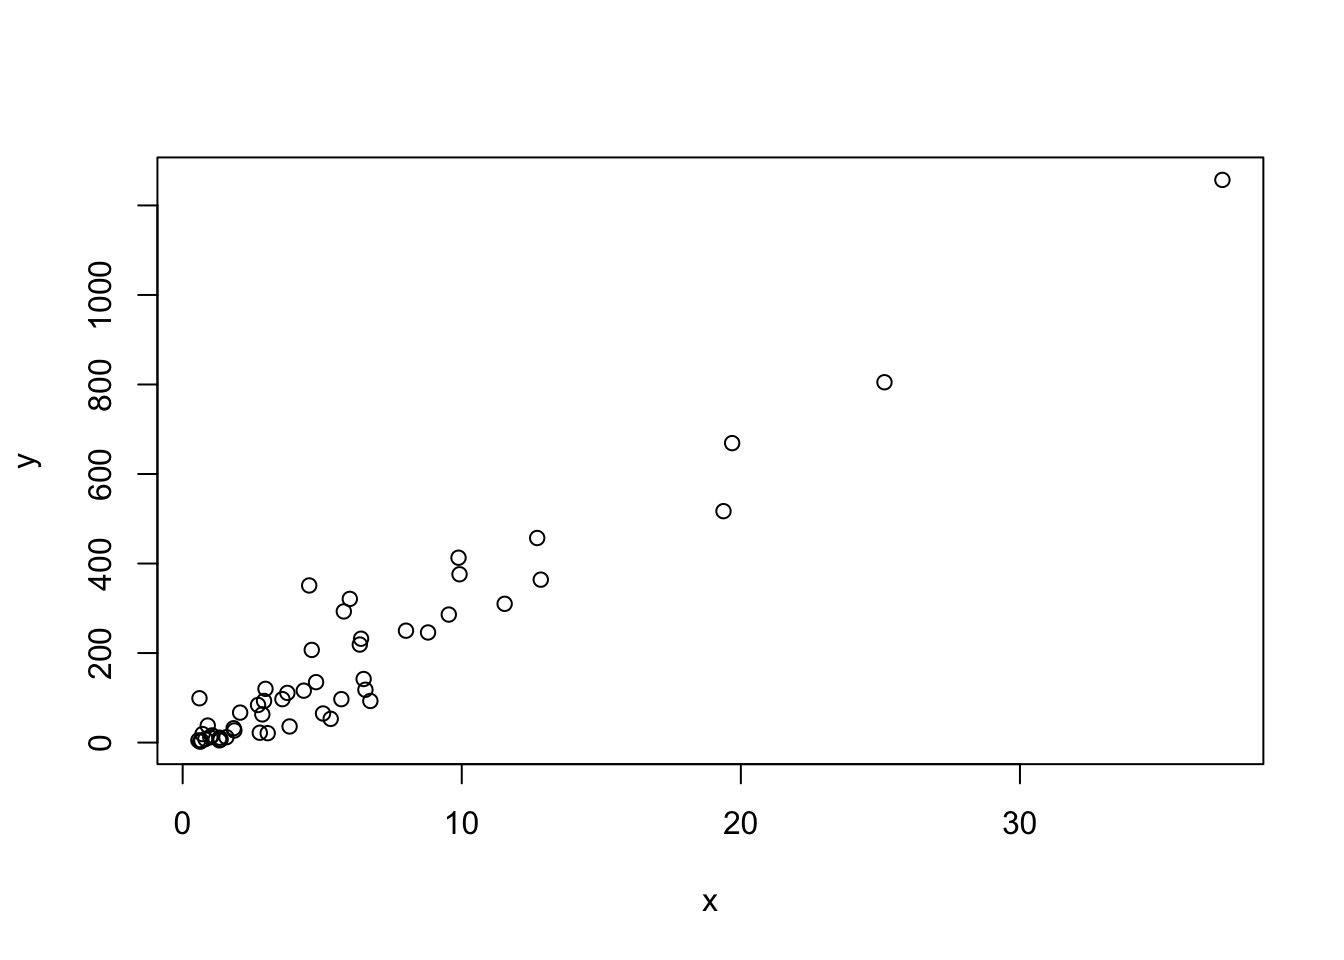
\includegraphics{Data_Science_R_Basics_files/figure-latex/unnamed-chunk-98-1.pdf}

\begin{Shaded}
\begin{Highlighting}[]
\CommentTok{# a histogram of murder rates}
\KeywordTok{hist}\NormalTok{(rate)}
\end{Highlighting}
\end{Shaded}

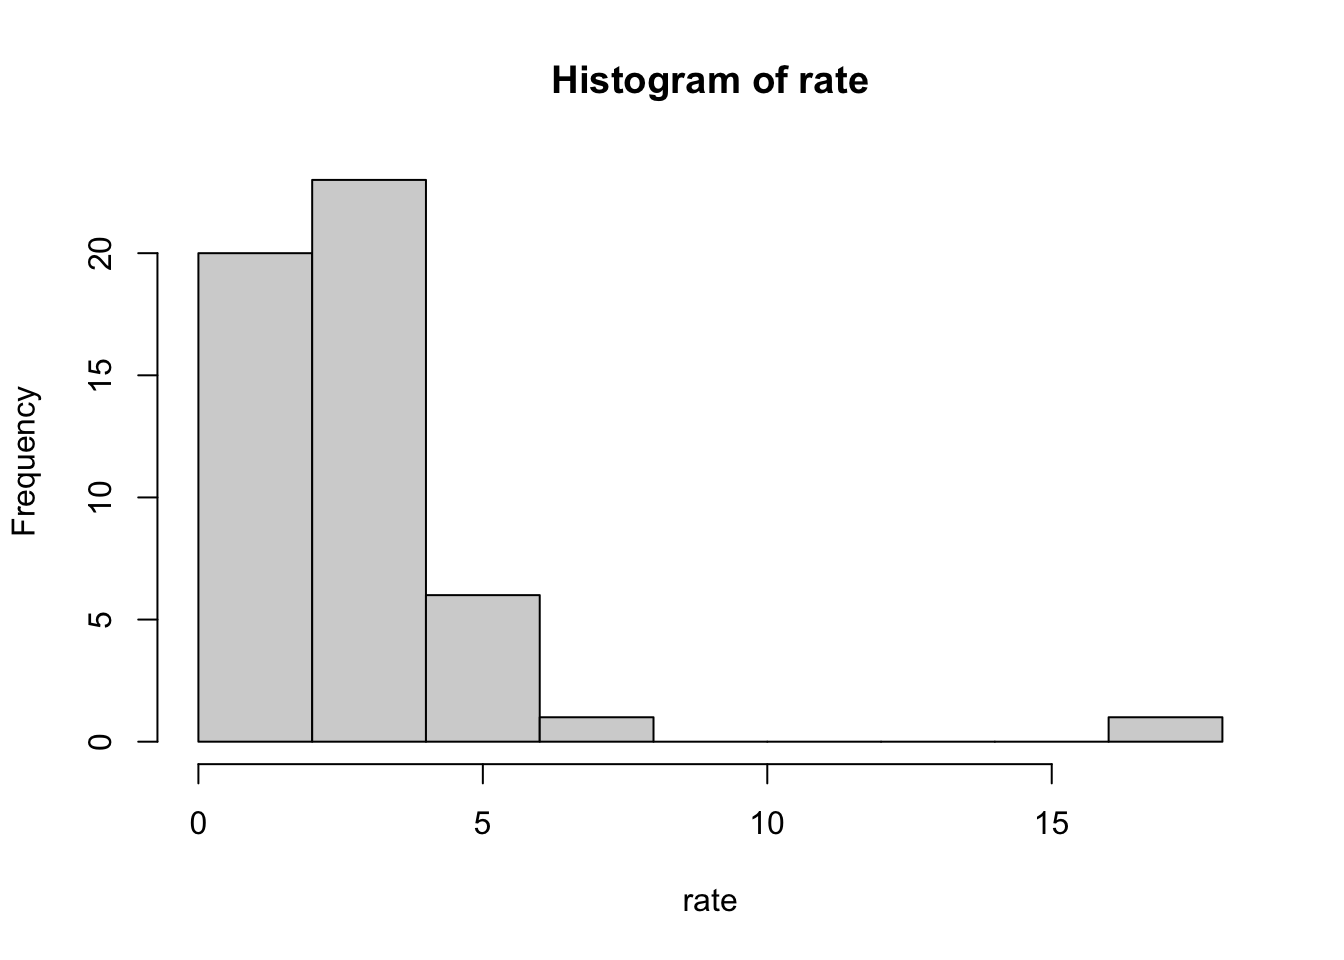
\includegraphics{Data_Science_R_Basics_files/figure-latex/unnamed-chunk-98-2.pdf}

\begin{Shaded}
\begin{Highlighting}[]
\CommentTok{# boxplots of murder rates by region}
\KeywordTok{boxplot}\NormalTok{(rate}\OperatorTok{~}\NormalTok{region, }\DataTypeTok{data =}\NormalTok{ murders)}
\end{Highlighting}
\end{Shaded}

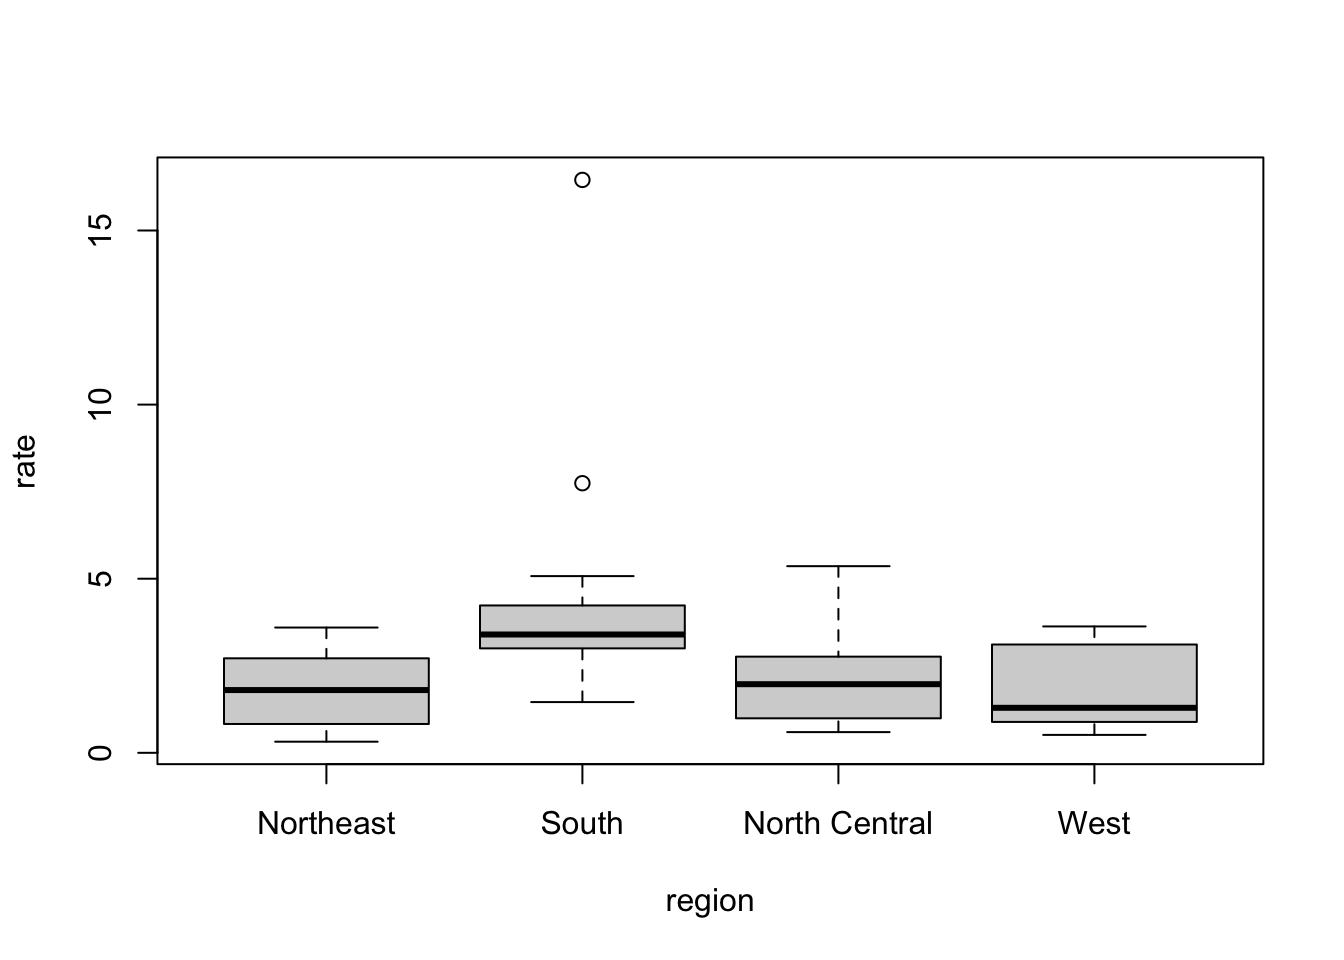
\includegraphics{Data_Science_R_Basics_files/figure-latex/unnamed-chunk-98-3.pdf}

\hypertarget{assessment---basic-plots}{%
\subsection{Assessment - Basic Plots}\label{assessment---basic-plots}}

\begin{enumerate}
\def\labelenumi{\arabic{enumi}.}
\tightlist
\item
  We made a plot of total murders versus population and noted a strong
  relationship: not surprisingly, states with larger populations had
  more murders.
\end{enumerate}

You can run the code in the console to get the plot.

\begin{Shaded}
\begin{Highlighting}[]
\KeywordTok{library}\NormalTok{(dslabs)}
\KeywordTok{data}\NormalTok{(murders)}

\NormalTok{population_in_millions <-}\StringTok{ }\NormalTok{murders}\OperatorTok{$}\NormalTok{population}\OperatorTok{/}\DecValTok{10}\OperatorTok{^}\DecValTok{6}
\NormalTok{total_gun_murders }\OperatorTok{<}\NormalTok{− murders}\OperatorTok{$}\NormalTok{total}

\KeywordTok{plot}\NormalTok{(population_in_millions, total_gun_murders)}
\end{Highlighting}
\end{Shaded}

Note that many states have populations below 5 million and are bunched
up in the plot. We may gain further insights from making this plot in
the log scale.

\begin{Shaded}
\begin{Highlighting}[]
\NormalTok{population_in_millions <-}\StringTok{ }\NormalTok{murders}\OperatorTok{$}\NormalTok{population}\OperatorTok{/}\DecValTok{10}\OperatorTok{^}\DecValTok{6}
\NormalTok{total_gun_murders <-}\StringTok{ }\NormalTok{murders}\OperatorTok{$}\NormalTok{total}

\KeywordTok{plot}\NormalTok{(population_in_millions, total_gun_murders)}
\end{Highlighting}
\end{Shaded}

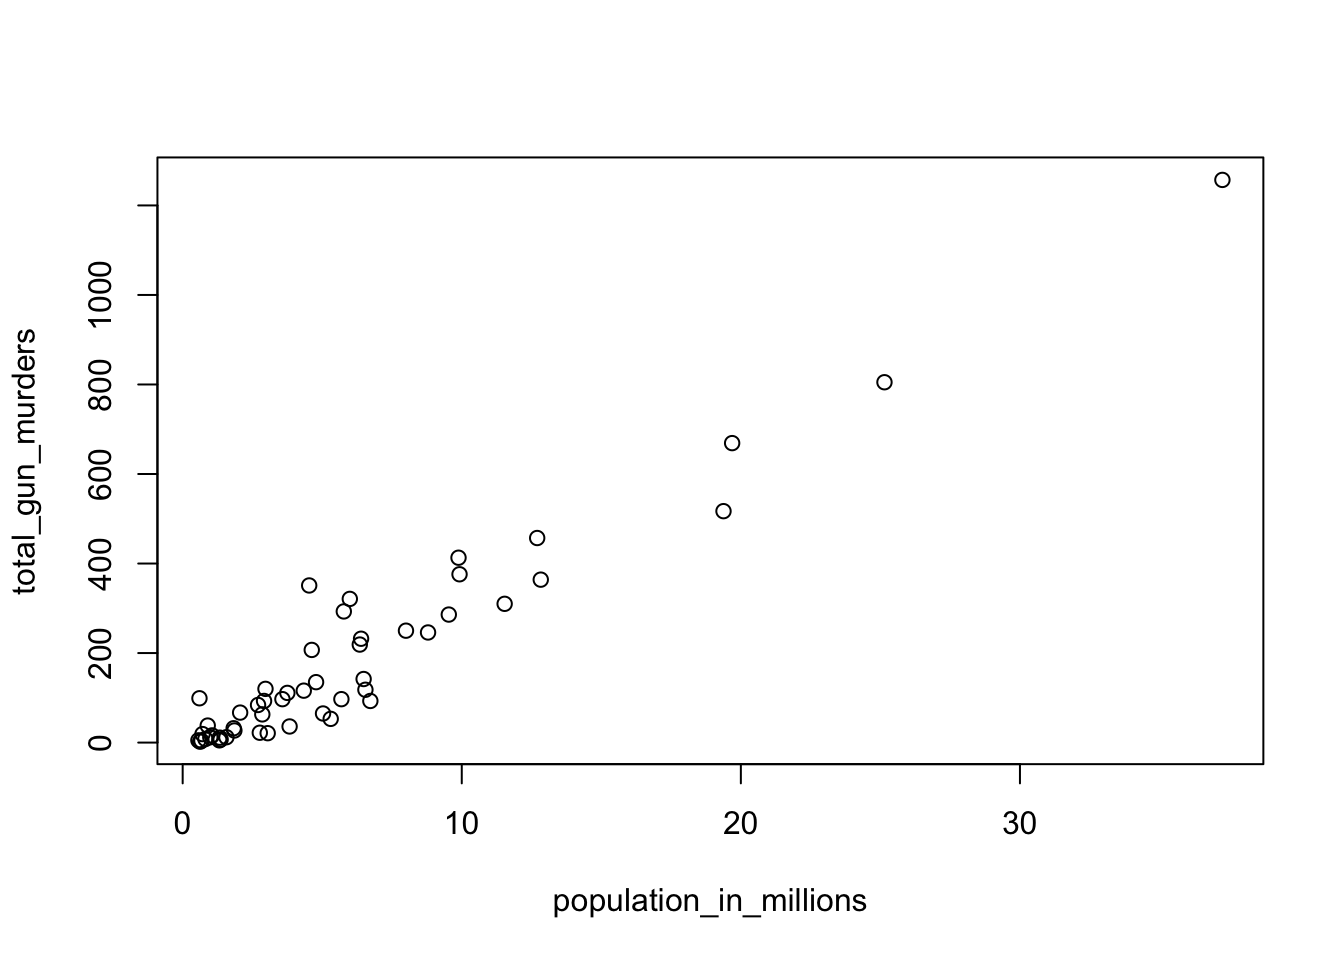
\includegraphics{Data_Science_R_Basics_files/figure-latex/unnamed-chunk-100-1.pdf}

\begin{Shaded}
\begin{Highlighting}[]
\CommentTok{# Transform population using the log10 transformation and save to object log10_population}
\NormalTok{log10_population <-}\StringTok{ }\KeywordTok{log10}\NormalTok{(murders}\OperatorTok{$}\NormalTok{population)}

\CommentTok{# Transform total gun murders using log10 transformation and save to object log10_total_gun_murders}
\NormalTok{log10_total_gun_murders <-}\StringTok{ }\KeywordTok{log10}\NormalTok{(total_gun_murders)}

\CommentTok{# Create a scatterplot with the log scale transformed population and murders }
\KeywordTok{plot}\NormalTok{(log10_population, log10_total_gun_murders)}
\end{Highlighting}
\end{Shaded}

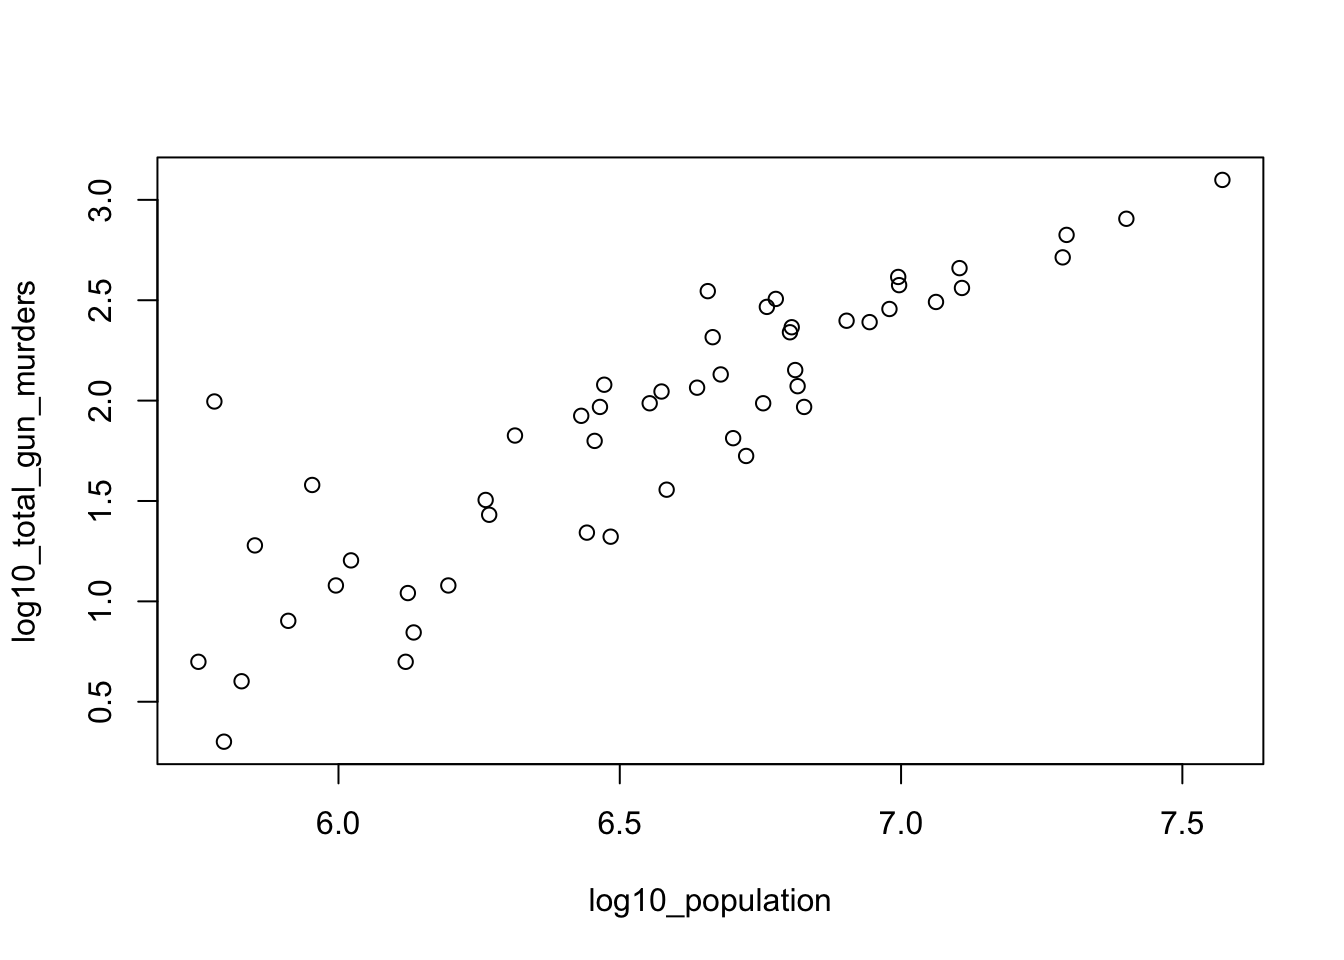
\includegraphics{Data_Science_R_Basics_files/figure-latex/unnamed-chunk-100-2.pdf}

\begin{enumerate}
\def\labelenumi{\arabic{enumi}.}
\setcounter{enumi}{1}
\tightlist
\item
  Now we are going to make a histogram.
\end{enumerate}

\begin{Shaded}
\begin{Highlighting}[]
\CommentTok{# Store the population in millions and save to population_in_millions }
\NormalTok{population_in_millions <-}\StringTok{ }\NormalTok{murders}\OperatorTok{$}\NormalTok{population}\OperatorTok{/}\DecValTok{10}\OperatorTok{^}\DecValTok{6}

\CommentTok{# Create a histogram of this variable}
\KeywordTok{hist}\NormalTok{(population_in_millions)}
\end{Highlighting}
\end{Shaded}

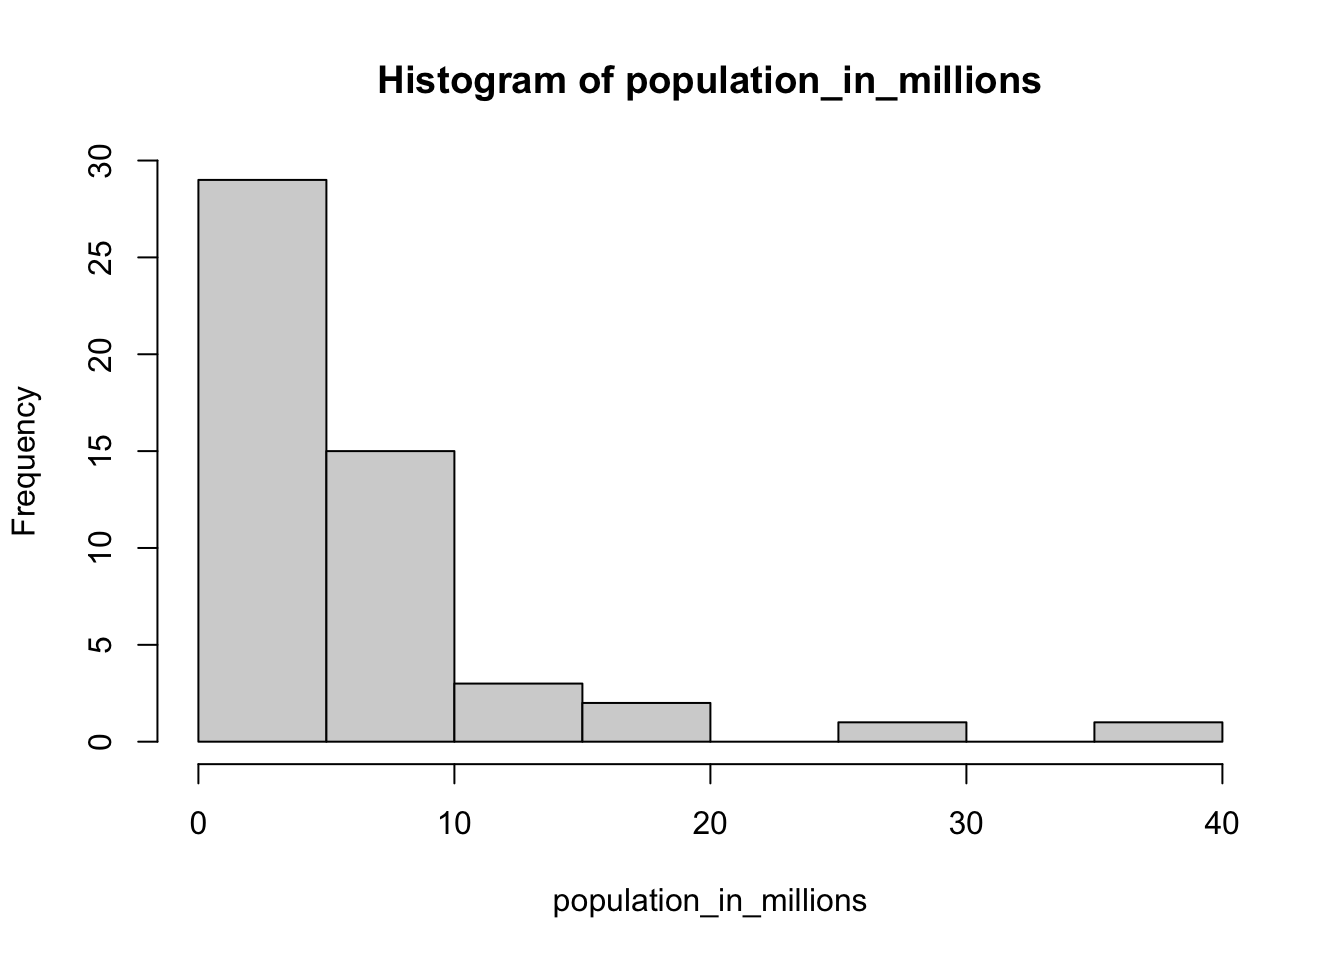
\includegraphics{Data_Science_R_Basics_files/figure-latex/unnamed-chunk-101-1.pdf}

\begin{enumerate}
\def\labelenumi{\arabic{enumi}.}
\setcounter{enumi}{2}
\tightlist
\item
  Now we are going to make boxplots. Boxplots are useful when we want a
  summary of several variables or several strata of the same variables.
  Making too many histograms can become too cumbersome.
\end{enumerate}

\begin{Shaded}
\begin{Highlighting}[]
\CommentTok{# Create a boxplot of state populations by region for the murders dataset}
\KeywordTok{boxplot}\NormalTok{(population}\OperatorTok{~}\NormalTok{region, }\DataTypeTok{data =}\NormalTok{ murders)}
\end{Highlighting}
\end{Shaded}

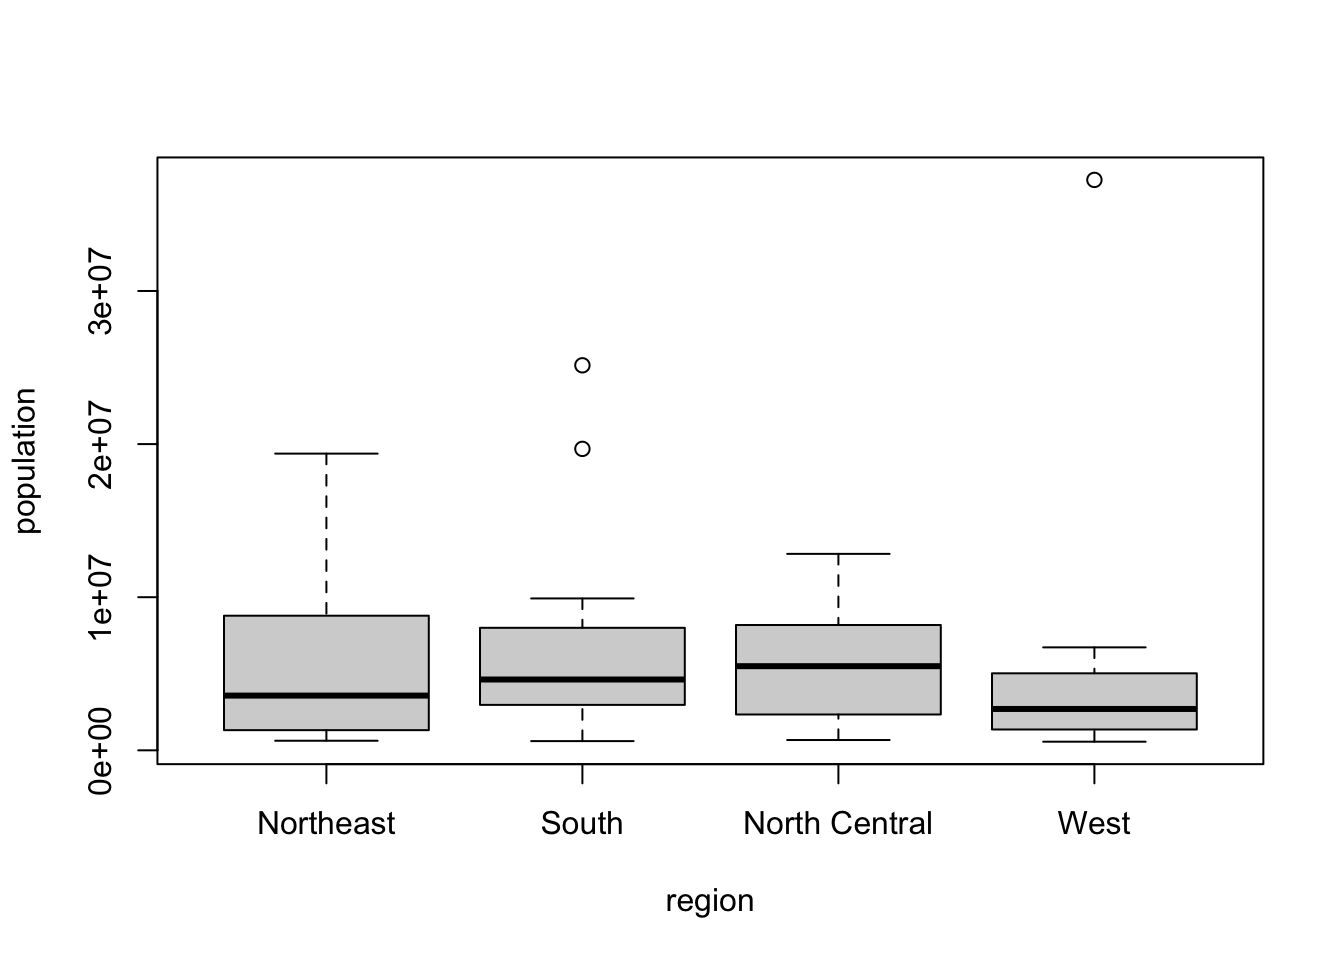
\includegraphics{Data_Science_R_Basics_files/figure-latex/unnamed-chunk-102-1.pdf}

\hypertarget{section-3-assessment}{%
\subsection{Section 3 Assessment}\label{section-3-assessment}}

\begin{Shaded}
\begin{Highlighting}[]
\KeywordTok{data}\NormalTok{(heights)}
\KeywordTok{options}\NormalTok{(}\DataTypeTok{digits =} \DecValTok{3}\NormalTok{)    }\CommentTok{# report 3 significant digits for all answers}
\end{Highlighting}
\end{Shaded}

\begin{enumerate}
\def\labelenumi{\arabic{enumi}.}
\tightlist
\item
  First, determine the average height in this dataset. Then create a
  logical vector \texttt{ind} with the indices for those individuals who
  are above average height.
\end{enumerate}

How many individuals in the dataset are above average height?

\begin{Shaded}
\begin{Highlighting}[]
\NormalTok{ind <-}\StringTok{ }\NormalTok{heights}\OperatorTok{$}\NormalTok{height }\OperatorTok{>}\StringTok{ }\KeywordTok{mean}\NormalTok{(heights}\OperatorTok{$}\NormalTok{height)}
\KeywordTok{sum}\NormalTok{(ind)}
\end{Highlighting}
\end{Shaded}

\begin{verbatim}
## [1] 532
\end{verbatim}

\begin{enumerate}
\def\labelenumi{\arabic{enumi}.}
\setcounter{enumi}{1}
\tightlist
\item
  How many individuals in the dataset are above average height and are
  female?
\end{enumerate}

\begin{Shaded}
\begin{Highlighting}[]
\KeywordTok{sum}\NormalTok{(ind }\OperatorTok{&}\StringTok{ }\NormalTok{heights}\OperatorTok{$}\NormalTok{sex}\OperatorTok{==}\StringTok{"Female"}\NormalTok{)}
\end{Highlighting}
\end{Shaded}

\begin{verbatim}
## [1] 31
\end{verbatim}

\begin{enumerate}
\def\labelenumi{\arabic{enumi}.}
\setcounter{enumi}{2}
\tightlist
\item
  If you use \texttt{mean} on a logical (TRUE/FALSE) vector, it returns
  the proportion of observations that are TRUE.
\end{enumerate}

What proportion of individuals in the dataset are female?

\begin{Shaded}
\begin{Highlighting}[]
\KeywordTok{mean}\NormalTok{(heights}\OperatorTok{$}\NormalTok{sex }\OperatorTok{==}\StringTok{ "Female"}\NormalTok{)}
\end{Highlighting}
\end{Shaded}

\begin{verbatim}
## [1] 0.227
\end{verbatim}

\begin{enumerate}
\def\labelenumi{\arabic{enumi}.}
\setcounter{enumi}{3}
\tightlist
\item
  This question takes you through three steps to determine the sex of
  the individual with the minimum height.
\end{enumerate}

Determine the minimum height in the \texttt{heights} dataset.

\begin{Shaded}
\begin{Highlighting}[]
\KeywordTok{min}\NormalTok{(heights}\OperatorTok{$}\NormalTok{height)}
\end{Highlighting}
\end{Shaded}

\begin{verbatim}
## [1] 50
\end{verbatim}

Use the \texttt{match()} function to determine the index of the
individual with the minimum height.

\begin{Shaded}
\begin{Highlighting}[]
\KeywordTok{match}\NormalTok{(}\DecValTok{50}\NormalTok{,heights}\OperatorTok{$}\NormalTok{height)}
\end{Highlighting}
\end{Shaded}

\begin{verbatim}
## [1] 1032
\end{verbatim}

Subset the \texttt{sex} column of the dataset by the index above to
determine the individual's sex. \texttt{Male}

\begin{Shaded}
\begin{Highlighting}[]
\NormalTok{heights}\OperatorTok{$}\NormalTok{sex[}\DecValTok{1032}\NormalTok{]}
\end{Highlighting}
\end{Shaded}

\begin{verbatim}
## [1] Male
## Levels: Female Male
\end{verbatim}

\begin{enumerate}
\def\labelenumi{\arabic{enumi}.}
\setcounter{enumi}{4}
\tightlist
\item
  This question takes you through three steps to determine how many of
  the integer height values between the minimum and maximum heights are
  not actual heights of individuals in the heights dataset.
\end{enumerate}

Determine the maximum height.

\begin{Shaded}
\begin{Highlighting}[]
\KeywordTok{max}\NormalTok{(heights}\OperatorTok{$}\NormalTok{height)}
\end{Highlighting}
\end{Shaded}

\begin{verbatim}
## [1] 82.7
\end{verbatim}

Which integer values are between the maximum and minimum heights? For
example, if the minimum height is 10.2 and the maximum height is 20.8,
your answer should be \texttt{x\ \textless{}-\ 11:20} to capture the
integers in between those values. (If either the maximum or minimum
height are integers, include those values too.)

Write code to create a vector x that includes the \emph{integers}
between the minimum and maximum heights.

\begin{Shaded}
\begin{Highlighting}[]
\NormalTok{x <-}\StringTok{ }\DecValTok{50}\OperatorTok{:}\DecValTok{82}
\end{Highlighting}
\end{Shaded}

How many of the integers in x are NOT heights in the dataset?

\begin{Shaded}
\begin{Highlighting}[]
\KeywordTok{sum}\NormalTok{(}\OperatorTok{!}\NormalTok{(x }\OperatorTok\StringTok{ }\NormalTok{heights}\OperatorTok{$}\NormalTok{height))}
\end{Highlighting}
\end{Shaded}

\begin{verbatim}
## [1] 3
\end{verbatim}

\begin{enumerate}
\def\labelenumi{\arabic{enumi}.}
\setcounter{enumi}{5}
\tightlist
\item
  Using the \texttt{heights} dataset, create a new column of heights in
  centimeters named \texttt{ht\_cm}. Recall that 1 inch = 2.54
  centimeters. Save the resulting dataset as \texttt{heights2}.
\end{enumerate}

What is the height in centimeters of the 18th individual (index 18)?

\begin{Shaded}
\begin{Highlighting}[]
\NormalTok{heights2 <-}\StringTok{ }\KeywordTok{mutate}\NormalTok{(heights, }\DataTypeTok{ht_cm =}\NormalTok{ height}\OperatorTok{*}\FloatTok{2.54}\NormalTok{)}

\CommentTok{# Then we subset the new heights2 dataset:}

\NormalTok{heights2}\OperatorTok{$}\NormalTok{ht_cm[}\DecValTok{18}\NormalTok{]}
\end{Highlighting}
\end{Shaded}

\begin{verbatim}
## [1] 163
\end{verbatim}

What is the mean height in centimeters?

\begin{Shaded}
\begin{Highlighting}[]
\KeywordTok{mean}\NormalTok{(heights2}\OperatorTok{$}\NormalTok{ht_cm)}
\end{Highlighting}
\end{Shaded}

\begin{verbatim}
## [1] 174
\end{verbatim}

Create a data frame \texttt{females} by filtering the \texttt{heights2}
data to contain only female individuals.

How many females are in the heights2 dataset?

\begin{Shaded}
\begin{Highlighting}[]
\NormalTok{females <-}\StringTok{ }\KeywordTok{filter}\NormalTok{(heights2, sex }\OperatorTok{==}\StringTok{ "Female"}\NormalTok{)}
\KeywordTok{nrow}\NormalTok{(females)}
\end{Highlighting}
\end{Shaded}

\begin{verbatim}
## [1] 238
\end{verbatim}

What is the mean height of the females in centimeters?

\begin{Shaded}
\begin{Highlighting}[]
\KeywordTok{mean}\NormalTok{(females}\OperatorTok{$}\NormalTok{ht_cm)}
\end{Highlighting}
\end{Shaded}

\begin{verbatim}
## [1] 165
\end{verbatim}

\begin{enumerate}
\def\labelenumi{\arabic{enumi}.}
\setcounter{enumi}{7}
\tightlist
\item
  The \texttt{olive} dataset in \textbf{dslabs} contains composition in
  percentage of eight fatty acids found in the lipid fraction of 572
  Italian olive oils:
\end{enumerate}

\begin{Shaded}
\begin{Highlighting}[]
\KeywordTok{data}\NormalTok{(olive)}
\KeywordTok{head}\NormalTok{(olive)}
\end{Highlighting}
\end{Shaded}

\begin{verbatim}
##           region         area palmitic palmitoleic stearic oleic linoleic
## 1 Southern Italy North-Apulia    10.75        0.75    2.26  78.2     6.72
## 2 Southern Italy North-Apulia    10.88        0.73    2.24  77.1     7.81
## 3 Southern Italy North-Apulia     9.11        0.54    2.46  81.1     5.49
## 4 Southern Italy North-Apulia     9.66        0.57    2.40  79.5     6.19
## 5 Southern Italy North-Apulia    10.51        0.67    2.59  77.7     6.72
## 6 Southern Italy North-Apulia     9.11        0.49    2.68  79.2     6.78
##   linolenic arachidic eicosenoic
## 1      0.36      0.60       0.29
## 2      0.31      0.61       0.29
## 3      0.31      0.63       0.29
## 4      0.50      0.78       0.35
## 5      0.50      0.80       0.46
## 6      0.51      0.70       0.44
\end{verbatim}

Plot the percent palmitic acid versus palmitoleic acid in a scatterplot.
What relationship do you see?

\begin{Shaded}
\begin{Highlighting}[]
\KeywordTok{plot}\NormalTok{(olive}\OperatorTok{$}\NormalTok{palmitic, olive}\OperatorTok{$}\NormalTok{palmitoleic)}
\end{Highlighting}
\end{Shaded}

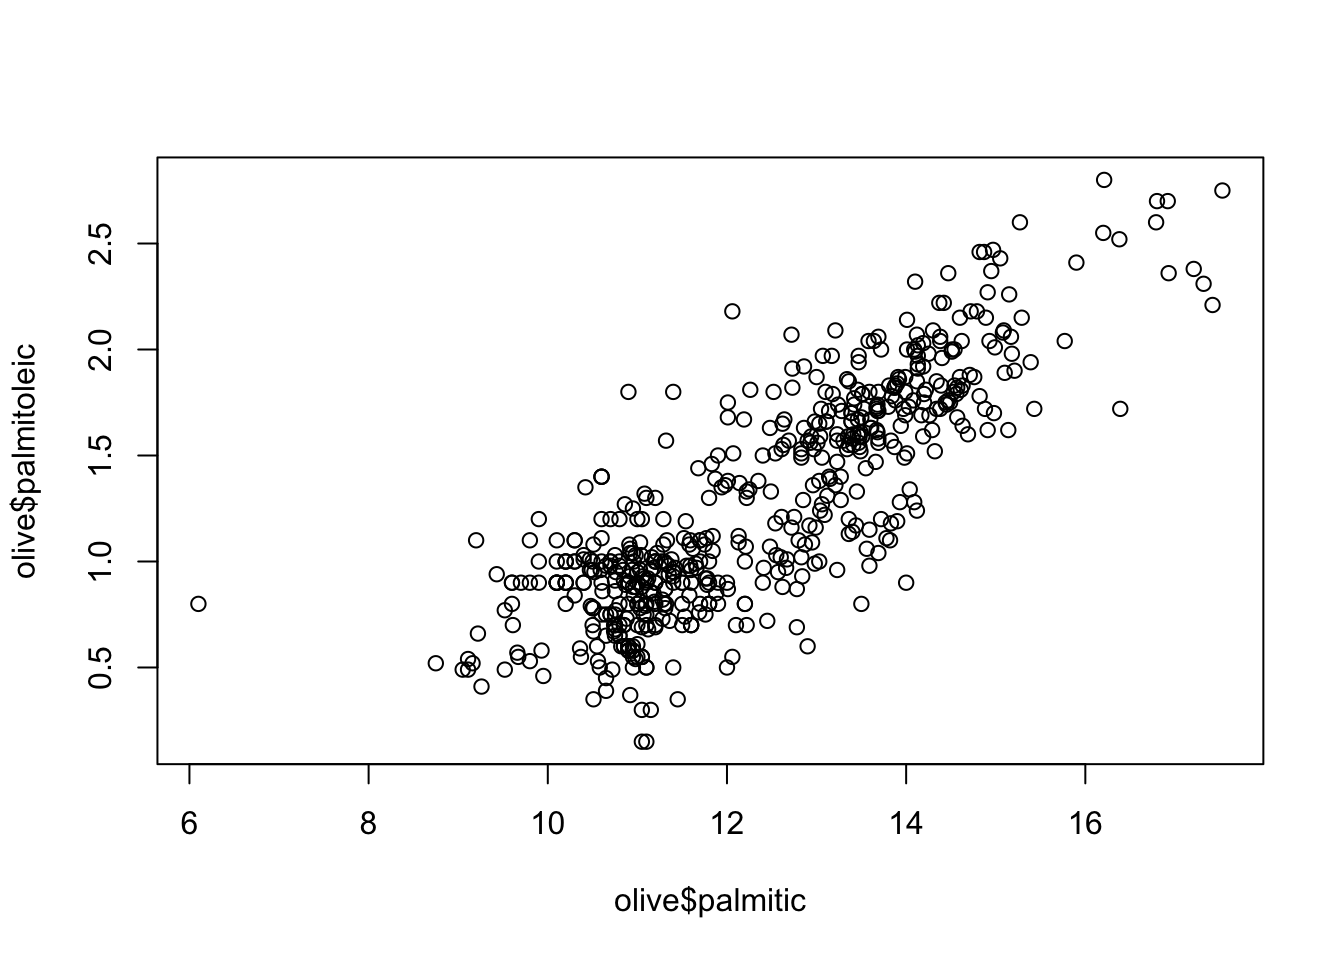
\includegraphics{Data_Science_R_Basics_files/figure-latex/unnamed-chunk-118-1.pdf}

\begin{itemize}
\tightlist
\item
  {[} {]} A. There is no relationship between palmitic and palmitoleic.
\item
  {[}X{]} B. There is a positive linear relationship between palmitic
  and palmitoleic.
\item
  {[} {]} C. There is a negative linear relationship between palmitic
  and palmitoleic.
\item
  {[} {]} D. There is a positive exponential relationship between
  palmitic and palmitoleic.
\item
  {[} {]} E. There is a negative exponential relationship between
  palmitic and palmitoleic.
\end{itemize}

\begin{enumerate}
\def\labelenumi{\arabic{enumi}.}
\setcounter{enumi}{8}
\tightlist
\item
  Create a histogram of the percentage of eicosenoic acid in
  \texttt{olive}. Which of the following is true?
\end{enumerate}

\begin{Shaded}
\begin{Highlighting}[]
\KeywordTok{hist}\NormalTok{(olive}\OperatorTok{$}\NormalTok{eicosenoic)}
\end{Highlighting}
\end{Shaded}

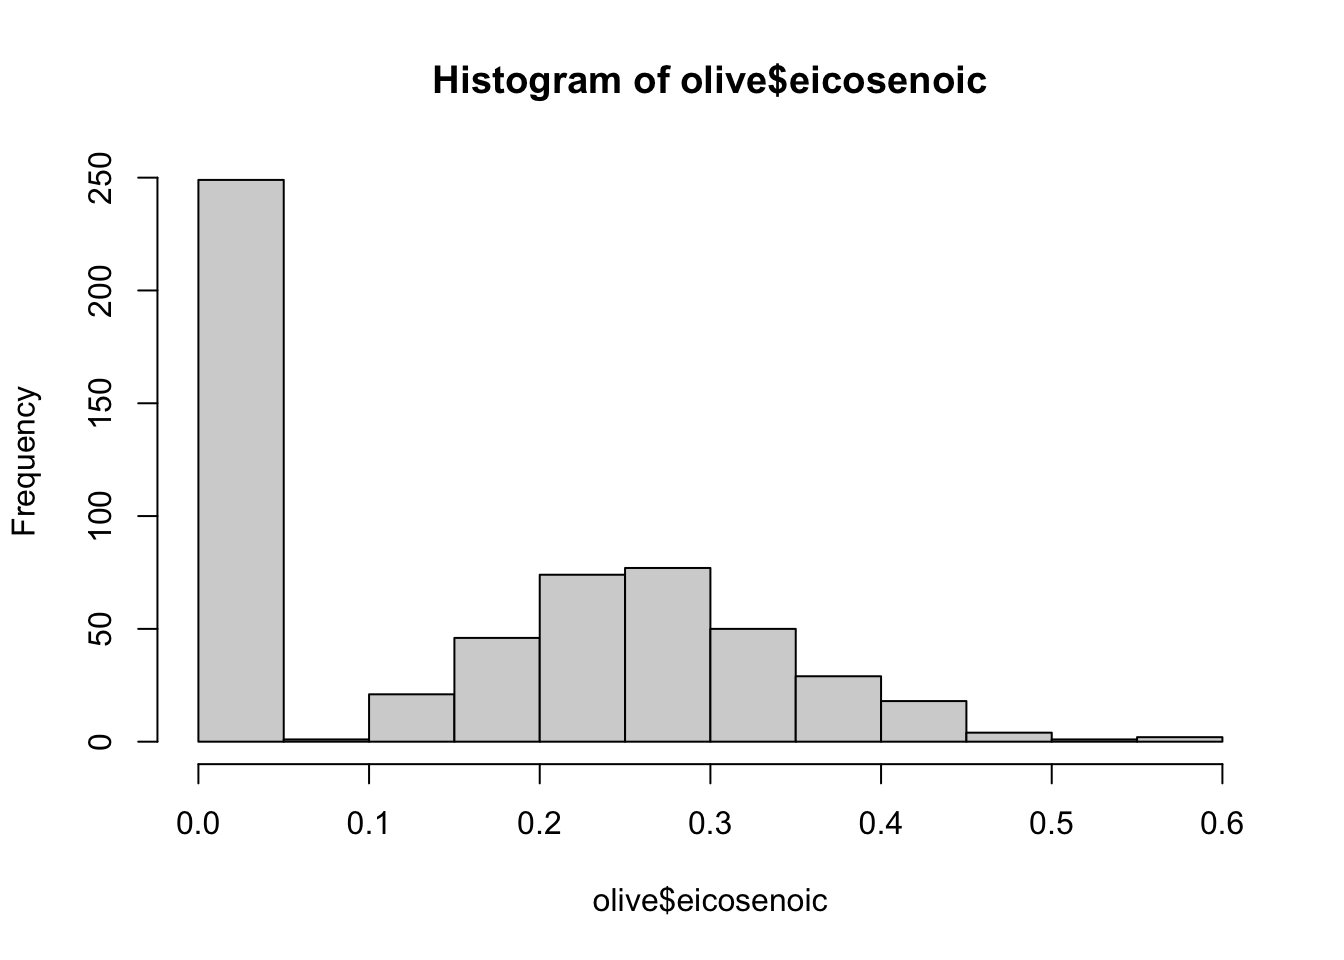
\includegraphics{Data_Science_R_Basics_files/figure-latex/unnamed-chunk-119-1.pdf}

\begin{itemize}
\tightlist
\item
  {[}X{]} A. The most common value of eicosenoic acid is below 0.05\%.
\item
  {[} {]} B. The most common value of eicosenoic acid is greater than
  0.5\%.
\item
  {[} {]} C. The most common value of eicosenoic acid is around 0.3\%.
\item
  {[} {]} D. There are equal numbers of olive oils with eicosenoic acid
  below 0.05\% and greater than 0.5\%.
\end{itemize}

\begin{enumerate}
\def\labelenumi{\arabic{enumi}.}
\setcounter{enumi}{9}
\tightlist
\item
  Make a boxplot of palmitic acid percentage in \texttt{olive} with
  separate distributions for each region.
\end{enumerate}

\begin{Shaded}
\begin{Highlighting}[]
\KeywordTok{boxplot}\NormalTok{(palmitic }\OperatorTok{~}\StringTok{ }\NormalTok{region, }\DataTypeTok{data =}\NormalTok{ olive)}
\end{Highlighting}
\end{Shaded}

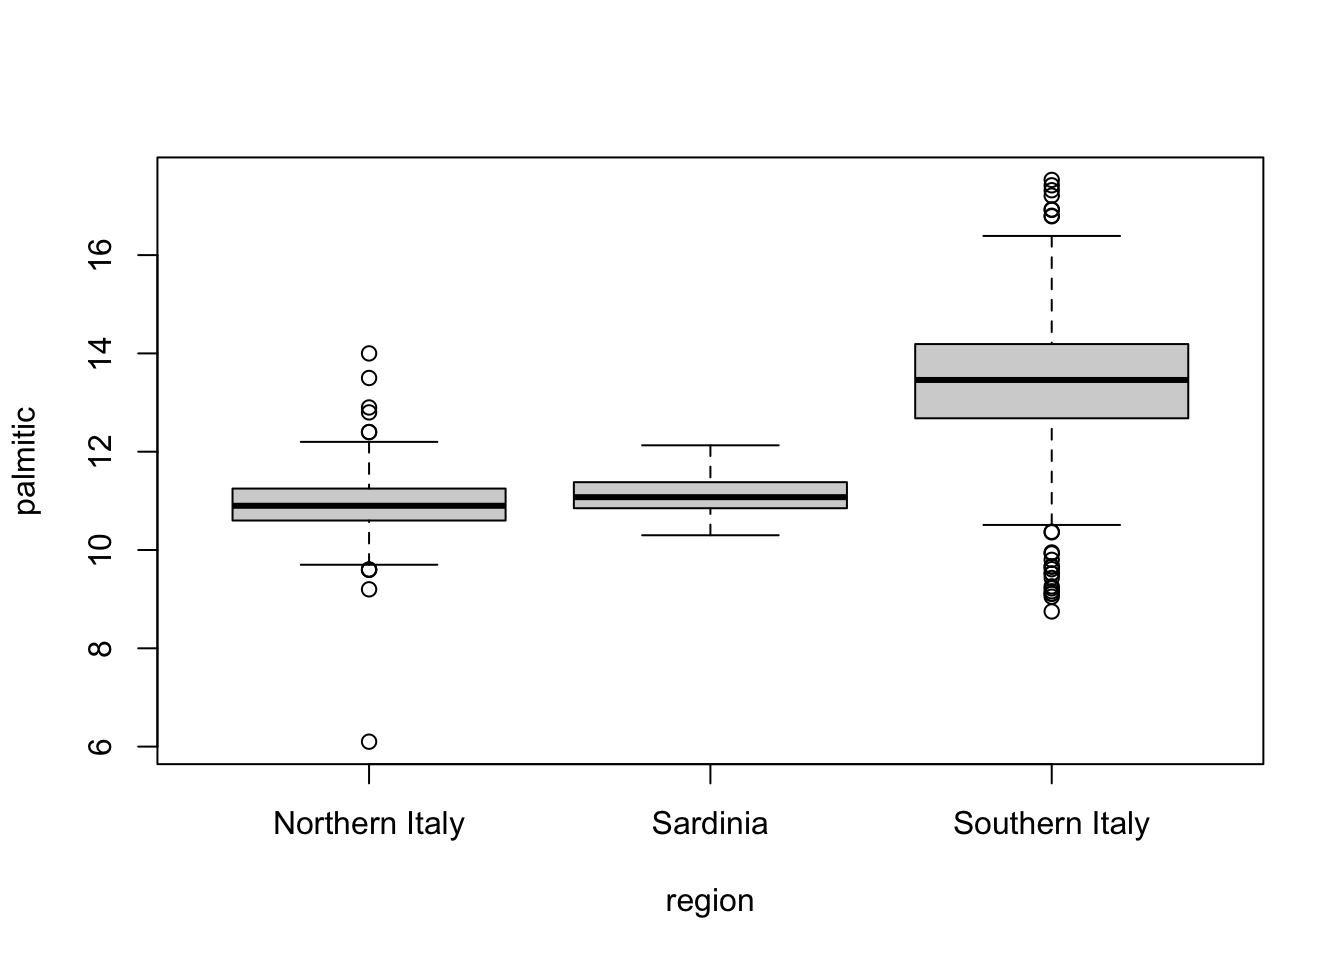
\includegraphics{Data_Science_R_Basics_files/figure-latex/unnamed-chunk-120-1.pdf}

Which region has the highest median palmitic acid percentage?
\texttt{Southern\ Italy}

Which region has the most variable palmitic acid percentage?
\texttt{Southern\ Italy}

\hypertarget{section-4-overview}{%
\subsection{Section 4 Overview}\label{section-4-overview}}

Section 4 introduces you to general programming features like `if-else',
and `for loop' commands so that you can write your own functions to
perform various operations on datasets.

In Section 4.1, you will:

\begin{itemize}
\tightlist
\item
  Understand some of the programming capabilities of R.
\end{itemize}

In Section 4.2, you will:

\begin{itemize}
\tightlist
\item
  Use basic conditional expressions to perform different operations.
\item
  Check if any or all elements of a logical vector are TRUE.
\end{itemize}

In Section 4.3, you will:

\begin{itemize}
\tightlist
\item
  Define and call functions to perform various operations.
\item
  Pass arguments to functions, and return variables/objects from
  functions.
\end{itemize}

In Section 4.4, you will:

\begin{itemize}
\tightlist
\item
  Use `for' loop to perform repeated operations.
\item
  Articulate in-built functions of R that you could try for yourself.
\end{itemize}

\hypertarget{programming-basics---introduction-to-programming-in-r}{%
\subsection{Programming Basics - Introduction to Programming in
R}\label{programming-basics---introduction-to-programming-in-r}}

The textbook for this section is available
\href{https://rafalab.github.io/dsbook/programming-basics.html}{here}

\hypertarget{basic-conditionals}{%
\subsection{Basic Conditionals}\label{basic-conditionals}}

The textbook for this section is available
\href{https://rafalab.github.io/dsbook/programming-basics.html\#conditionals}{here}

\textbf{Key Points}

\begin{itemize}
\tightlist
\item
  The most common conditional expression in programming is an if-else
  statement, which has the form ``if {[}condition{]}, perform
  {[}expression{]}, else perform {[}alternative expression{]}''.
\item
  The \texttt{ifelse()} function works similarly to an if-else
  statement, but it is particularly useful since it works on vectors by
  examining each element of the vector and returning a corresponding
  answer accordingly.
\item
  The \texttt{any()} function takes a vector of logicals and returns
  true if any of the entries are true.
\item
  The \texttt{all()} function takes a vector of logicals and returns
  true if all of the entries are true.
\end{itemize}

\emph{Code}

\begin{Shaded}
\begin{Highlighting}[]
\CommentTok{# an example showing the general structure of an if-else statement}
\NormalTok{a <-}\StringTok{ }\DecValTok{0}
\ControlFlowTok{if}\NormalTok{(a}\OperatorTok{!=}\DecValTok{0}\NormalTok{)\{}
  \KeywordTok{print}\NormalTok{(}\DecValTok{1}\OperatorTok{/}\NormalTok{a)}
\NormalTok{\} }\ControlFlowTok{else}\NormalTok{\{}
  \KeywordTok{print}\NormalTok{(}\StringTok{"No reciprocal for 0."}\NormalTok{)}
\NormalTok{\}}
\end{Highlighting}
\end{Shaded}

\begin{verbatim}
## [1] "No reciprocal for 0."
\end{verbatim}

\begin{Shaded}
\begin{Highlighting}[]
\CommentTok{# an example that tells us which states, if any, have a murder rate less than 0.5}
\KeywordTok{library}\NormalTok{(dslabs)}
\KeywordTok{data}\NormalTok{(murders)}
\NormalTok{murder_rate <-}\StringTok{ }\NormalTok{murders}\OperatorTok{$}\NormalTok{total }\OperatorTok{/}\StringTok{ }\NormalTok{murders}\OperatorTok{$}\NormalTok{population}\OperatorTok{*}\DecValTok{100000}
\NormalTok{ind <-}\StringTok{ }\KeywordTok{which.min}\NormalTok{(murder_rate)}
\ControlFlowTok{if}\NormalTok{(murder_rate[ind] }\OperatorTok{<}\StringTok{ }\FloatTok{0.5}\NormalTok{)\{}
  \KeywordTok{print}\NormalTok{(murders}\OperatorTok{$}\NormalTok{state[ind]) }
\NormalTok{\} }\ControlFlowTok{else}\NormalTok{\{}
  \KeywordTok{print}\NormalTok{(}\StringTok{"No state has murder rate that low"}\NormalTok{)}
\NormalTok{\}}
\end{Highlighting}
\end{Shaded}

\begin{verbatim}
## [1] "Vermont"
\end{verbatim}

\begin{Shaded}
\begin{Highlighting}[]
\CommentTok{# changing the condition to < 0.25 changes the result}
\ControlFlowTok{if}\NormalTok{(murder_rate[ind] }\OperatorTok{<}\StringTok{ }\FloatTok{0.25}\NormalTok{)\{}
  \KeywordTok{print}\NormalTok{(murders}\OperatorTok{$}\NormalTok{state[ind]) }
\NormalTok{\} }\ControlFlowTok{else}\NormalTok{\{}
  \KeywordTok{print}\NormalTok{(}\StringTok{"No state has a murder rate that low."}\NormalTok{)}
\NormalTok{\}}
\end{Highlighting}
\end{Shaded}

\begin{verbatim}
## [1] "No state has a murder rate that low."
\end{verbatim}

\begin{Shaded}
\begin{Highlighting}[]
\CommentTok{# the ifelse() function works similarly to an if-else conditional}
\NormalTok{a <-}\StringTok{ }\DecValTok{0}
\KeywordTok{ifelse}\NormalTok{(a }\OperatorTok{>}\StringTok{ }\DecValTok{0}\NormalTok{, }\DecValTok{1}\OperatorTok{/}\NormalTok{a, }\OtherTok{NA}\NormalTok{)}
\end{Highlighting}
\end{Shaded}

\begin{verbatim}
## [1] NA
\end{verbatim}

\begin{Shaded}
\begin{Highlighting}[]
\CommentTok{# the ifelse() function is particularly useful on vectors}
\NormalTok{a <-}\StringTok{ }\KeywordTok{c}\NormalTok{(}\DecValTok{0}\NormalTok{,}\DecValTok{1}\NormalTok{,}\DecValTok{2}\NormalTok{,}\OperatorTok{-}\DecValTok{4}\NormalTok{,}\DecValTok{5}\NormalTok{)}
\NormalTok{result <-}\StringTok{ }\KeywordTok{ifelse}\NormalTok{(a }\OperatorTok{>}\StringTok{ }\DecValTok{0}\NormalTok{, }\DecValTok{1}\OperatorTok{/}\NormalTok{a, }\OtherTok{NA}\NormalTok{)}

\CommentTok{# the ifelse() function is also helpful for replacing missing values}
\KeywordTok{data}\NormalTok{(na_example)}
\NormalTok{no_nas <-}\StringTok{ }\KeywordTok{ifelse}\NormalTok{(}\KeywordTok{is.na}\NormalTok{(na_example), }\DecValTok{0}\NormalTok{, na_example) }
\KeywordTok{sum}\NormalTok{(}\KeywordTok{is.na}\NormalTok{(no_nas))}
\end{Highlighting}
\end{Shaded}

\begin{verbatim}
## [1] 0
\end{verbatim}

\begin{Shaded}
\begin{Highlighting}[]
\CommentTok{# the any() and all() functions evaluate logical vectors}
\NormalTok{z <-}\StringTok{ }\KeywordTok{c}\NormalTok{(}\OtherTok{TRUE}\NormalTok{, }\OtherTok{TRUE}\NormalTok{, }\OtherTok{FALSE}\NormalTok{)}
\KeywordTok{any}\NormalTok{(z)}
\end{Highlighting}
\end{Shaded}

\begin{verbatim}
## [1] TRUE
\end{verbatim}

\begin{Shaded}
\begin{Highlighting}[]
\KeywordTok{all}\NormalTok{(z)}
\end{Highlighting}
\end{Shaded}

\begin{verbatim}
## [1] FALSE
\end{verbatim}

\hypertarget{functions}{%
\subsection{Functions}\label{functions}}

The textbook for this section is available
\href{https://rafalab.github.io/dsbook/programming-basics.html\#defining-functions}{here}

\textbf{Key points}

\begin{itemize}
\tightlist
\item
  The R function, called \texttt{function()} tells R you are about to
  define a new function.
\item
  Functions are objects, so must be assigned a variable name with the
  arrow operator.
\item
  The general way to define functions is: (1) decide the function name,
  which will be an object, (2) type \texttt{function()} with your
  function's arguments in parentheses, (3) write all the operations
  inside brackets.
\item
  Variables defined inside a function are not saved in the workspace.
\end{itemize}

\emph{Code}

\begin{Shaded}
\begin{Highlighting}[]
\CommentTok{# example of defining a function to compute the average of a vector x}
\NormalTok{avg <-}\StringTok{ }\ControlFlowTok{function}\NormalTok{(x)\{}
\NormalTok{  s <-}\StringTok{ }\KeywordTok{sum}\NormalTok{(x)}
\NormalTok{  n <-}\StringTok{ }\KeywordTok{length}\NormalTok{(x)}
\NormalTok{  s}\OperatorTok{/}\NormalTok{n}
\NormalTok{\}}

\CommentTok{# we see that the above function and the pre-built R mean() function are identical}
\NormalTok{x <-}\StringTok{ }\DecValTok{1}\OperatorTok{:}\DecValTok{100}
\KeywordTok{identical}\NormalTok{(}\KeywordTok{mean}\NormalTok{(x), }\KeywordTok{avg}\NormalTok{(x))}
\end{Highlighting}
\end{Shaded}

\begin{verbatim}
## [1] TRUE
\end{verbatim}

\begin{Shaded}
\begin{Highlighting}[]
\CommentTok{# variables inside a function are not defined in the workspace}
\NormalTok{s <-}\StringTok{ }\DecValTok{3}
\KeywordTok{avg}\NormalTok{(}\DecValTok{1}\OperatorTok{:}\DecValTok{10}\NormalTok{)}
\end{Highlighting}
\end{Shaded}

\begin{verbatim}
## [1] 5.5
\end{verbatim}

\begin{Shaded}
\begin{Highlighting}[]
\NormalTok{s}
\end{Highlighting}
\end{Shaded}

\begin{verbatim}
## [1] 3
\end{verbatim}

\begin{Shaded}
\begin{Highlighting}[]
\CommentTok{# the general form of a function}
\NormalTok{my_function <-}\StringTok{ }\ControlFlowTok{function}\NormalTok{(VARIABLE_NAME)\{}
\NormalTok{  perform operations on VARIABLE_NAME and calculate VALUE}
\NormalTok{  VALUE}
\NormalTok{\}}
\end{Highlighting}
\end{Shaded}

\begin{Shaded}
\begin{Highlighting}[]
\CommentTok{# functions can have multiple arguments as well as default values}
\NormalTok{avg <-}\StringTok{ }\ControlFlowTok{function}\NormalTok{(x, }\DataTypeTok{arithmetic =} \OtherTok{TRUE}\NormalTok{)\{}
\NormalTok{  n <-}\StringTok{ }\KeywordTok{length}\NormalTok{(x)}
  \KeywordTok{ifelse}\NormalTok{(arithmetic, }\KeywordTok{sum}\NormalTok{(x)}\OperatorTok{/}\NormalTok{n, }\KeywordTok{prod}\NormalTok{(x)}\OperatorTok{^}\NormalTok{(}\DecValTok{1}\OperatorTok{/}\NormalTok{n))}
\NormalTok{\}}
\end{Highlighting}
\end{Shaded}

\hypertarget{for-loops}{%
\subsection{For Loops}\label{for-loops}}

The textbook for this section is available
\href{https://rafalab.github.io/dsbook/programming-basics.html\#for-loops}{here}

\textbf{Key points}

\begin{itemize}
\tightlist
\item
  For-loops perform the same task over and over while changing the
  variable. They let us define the range that our variable takes, and
  then changes the value with each loop and evaluates the expression
  every time inside the loop.
\item
  The general form of a for-loop is: ``For i in {[}some range{]}, do
  operations''. This i changes across the range of values and the
  operations assume i is a value you're interested in computing on.
\item
  At the end of the loop, the value of i is the last value of the range.
\end{itemize}

\emph{Code}

\begin{Shaded}
\begin{Highlighting}[]
\CommentTok{# creating a function that computes the sum of integers 1 through n}
\NormalTok{compute_s_n <-}\StringTok{ }\ControlFlowTok{function}\NormalTok{(n)\{}
\NormalTok{  x <-}\StringTok{ }\DecValTok{1}\OperatorTok{:}\NormalTok{n}
  \KeywordTok{sum}\NormalTok{(x)}
\NormalTok{\}}

\CommentTok{# a very simple for-loop}
\ControlFlowTok{for}\NormalTok{(i }\ControlFlowTok{in} \DecValTok{1}\OperatorTok{:}\DecValTok{5}\NormalTok{)\{}
  \KeywordTok{print}\NormalTok{(i)}
\NormalTok{\}}
\end{Highlighting}
\end{Shaded}

\begin{verbatim}
## [1] 1
## [1] 2
## [1] 3
## [1] 4
## [1] 5
\end{verbatim}

\begin{Shaded}
\begin{Highlighting}[]
\CommentTok{# a for-loop for our summation}
\NormalTok{m <-}\StringTok{ }\DecValTok{25}
\NormalTok{s_n <-}\StringTok{ }\KeywordTok{vector}\NormalTok{(}\DataTypeTok{length =}\NormalTok{ m) }\CommentTok{# create an empty vector}
\ControlFlowTok{for}\NormalTok{(n }\ControlFlowTok{in} \DecValTok{1}\OperatorTok{:}\NormalTok{m)\{}
\NormalTok{  s_n[n] <-}\StringTok{ }\KeywordTok{compute_s_n}\NormalTok{(n)}
\NormalTok{\}}

\CommentTok{# creating a plot for our summation function}
\NormalTok{n <-}\StringTok{ }\DecValTok{1}\OperatorTok{:}\NormalTok{m}
\KeywordTok{plot}\NormalTok{(n, s_n)}

\CommentTok{# a table of values comparing our function to the summation formula}
\KeywordTok{head}\NormalTok{(}\KeywordTok{data.frame}\NormalTok{(}\DataTypeTok{s_n =}\NormalTok{ s_n, }\DataTypeTok{formula =}\NormalTok{ n}\OperatorTok{*}\NormalTok{(n}\OperatorTok{+}\DecValTok{1}\NormalTok{)}\OperatorTok{/}\DecValTok{2}\NormalTok{))}
\end{Highlighting}
\end{Shaded}

\begin{verbatim}
##   s_n formula
## 1   1       1
## 2   3       3
## 3   6       6
## 4  10      10
## 5  15      15
## 6  21      21
\end{verbatim}

\begin{Shaded}
\begin{Highlighting}[]
\CommentTok{# overlaying our function with the summation formula}
\KeywordTok{plot}\NormalTok{(n, s_n)}
\KeywordTok{lines}\NormalTok{(n, n}\OperatorTok{*}\NormalTok{(n}\OperatorTok{+}\DecValTok{1}\NormalTok{)}\OperatorTok{/}\DecValTok{2}\NormalTok{)}
\end{Highlighting}
\end{Shaded}

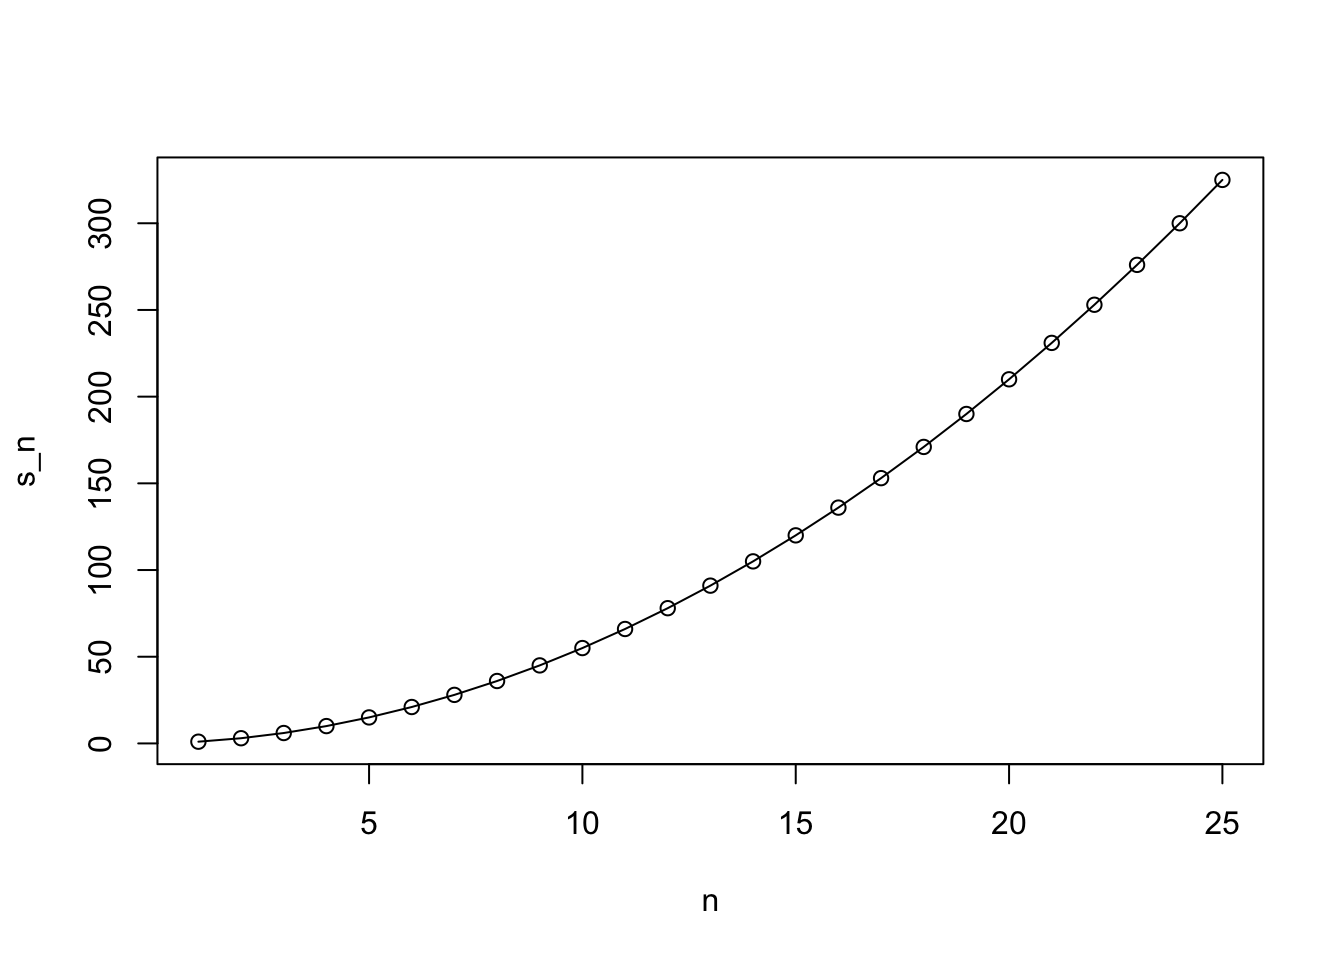
\includegraphics{Data_Science_R_Basics_files/figure-latex/unnamed-chunk-125-1.pdf}

\hypertarget{assessment---programming-basics}{%
\subsection{Assessment - Programming
Basics}\label{assessment---programming-basics}}

\begin{enumerate}
\def\labelenumi{\arabic{enumi}.}
\tightlist
\item
  What will this conditional expression return?
\end{enumerate}

\begin{Shaded}
\begin{Highlighting}[]
\NormalTok{x <-}\StringTok{ }\KeywordTok{c}\NormalTok{(}\DecValTok{1}\NormalTok{,}\DecValTok{2}\NormalTok{,}\OperatorTok{-}\DecValTok{3}\NormalTok{,}\DecValTok{4}\NormalTok{)}
\ControlFlowTok{if}\NormalTok{(}\KeywordTok{all}\NormalTok{(x}\OperatorTok{>}\DecValTok{0}\NormalTok{))\{}
\KeywordTok{print}\NormalTok{(}\StringTok{"All Postives"}\NormalTok{)}
\NormalTok{\} }\ControlFlowTok{else}\NormalTok{\{}
\KeywordTok{print}\NormalTok{(}\StringTok{"Not all positives"}\NormalTok{)}
\NormalTok{\}}
\end{Highlighting}
\end{Shaded}

\begin{verbatim}
## [1] "Not all positives"
\end{verbatim}

\begin{itemize}
\tightlist
\item
  {[} {]} A. All Positives
\item
  {[}X{]} B. Not All Positives
\item
  {[} {]} C. N/A
\item
  {[} {]} D. None of the above
\end{itemize}

\begin{enumerate}
\def\labelenumi{\arabic{enumi}.}
\setcounter{enumi}{1}
\tightlist
\item
  Which of the following expressions is always FALSE when at least one
  entry of a logical vector x is TRUE?
\end{enumerate}

\begin{itemize}
\tightlist
\item
  {[} {]} A. all(x)
\item
  {[} {]} B. any(x)
\item
  {[} {]} C. any(!x)
\item
  {[}X{]} D. all(!x)
\end{itemize}

\begin{enumerate}
\def\labelenumi{\arabic{enumi}.}
\setcounter{enumi}{2}
\tightlist
\item
  The function nchar tells you how many characters long a character
  vector is.
\end{enumerate}

Write a line of code that assigns to the object new\_names the state
abbreviation when the state name is longer than 8 characters.

\begin{verbatim}
# Assign the state abbreviation when the state name is longer than 8 characters 
new_names <- ifelse(nchar(murders$state)>8, murders$abb, murders$state)
\end{verbatim}

\begin{enumerate}
\def\labelenumi{\arabic{enumi}.}
\setcounter{enumi}{3}
\tightlist
\item
  Create a function sum\_n that for any given value, say n, computes the
  sum of the integers from 1 to n (inclusive). Use the function to
  determine the sum of integers from 1 to 5,000.
\end{enumerate}

\begin{verbatim}
# Create function called `sum_n`
sum_n <- function(n){
  sum(1:n)
}
# Use the function to determine the sum of integers from 1 to 5000
sum_n(5000)
\end{verbatim}

\begin{verbatim}
## [1] 12502500
\end{verbatim}

\begin{enumerate}
\def\labelenumi{\arabic{enumi}.}
\setcounter{enumi}{4}
\tightlist
\item
  Create a function altman\_plot that takes two arguments, x and y, and
  plots the difference against the sum.
\end{enumerate}

\begin{verbatim}
# Create `altman_plot` 
altman_plot <- function(x,y) {
  plot(x+y,y-x)
}
\end{verbatim}

\begin{enumerate}
\def\labelenumi{\arabic{enumi}.}
\setcounter{enumi}{5}
\tightlist
\item
  After running the code below, what is the value of x?
\end{enumerate}

\begin{verbatim}
x <- 3
my_func <- function(y){
x <- 5
y+5
}
\end{verbatim}

\begin{verbatim}
# Run this code 
x <- 3
    my_func <- function(y){
    x <- 5
    y+5
}

# Print value of x 
print(x)
\end{verbatim}

\begin{verbatim}
## [1] 3
\end{verbatim}

\begin{enumerate}
\def\labelenumi{\arabic{enumi}.}
\setcounter{enumi}{6}
\tightlist
\item
  Write a function compute\_s\_n that for any given n computes the sum
  S\_n = 1\^{}2 + 2\^{}2 + 3\^{}2 + . n\^{}2. Report the value of the
  sum when n = 10.
\end{enumerate}

\begin{verbatim}
# Here is an example of function that adds numbers from 1 to n
example_func <- function(n){
    x <- 1:n
    sum(x)
}

# Here is the sum of the first 100 numbers
example_func(100)
\end{verbatim}

\begin{verbatim}
## [1] 5050
\end{verbatim}

\begin{verbatim}
# Write a function compute_s_n that with argument n and returns of 1 + 2^2 + ...+ n^2
compute_s_n <- function(n){
  x <- 1:n
  sum(x^2)
}
# Report the value of the sum when n=10
compute_s_n(10)
\end{verbatim}

\begin{verbatim}
## [1] 385
\end{verbatim}

\begin{enumerate}
\def\labelenumi{\arabic{enumi}.}
\setcounter{enumi}{7}
\tightlist
\item
  Define an empty numerical vector s\_n of size 25 using s\_n
  \textless{}- vector(``numeric'', 25) and store in the results of S\_1,
  S\_2, . S\_25 using a for-loop.
\end{enumerate}

\begin{verbatim}
# Define a function and store it in `compute_s_n`
compute_s_n <- function(n){
  x <- 1:n
  sum(x^2)
}

# Create a vector for storing results
s_n <- vector("numeric", 25)

# write a for-loop to store the results in s_n
for(i in 1:25){
  s_n[i] <- compute_s_n(i)
}
\end{verbatim}

\begin{enumerate}
\def\labelenumi{\arabic{enumi}.}
\setcounter{enumi}{8}
\tightlist
\item
  If we do the math, we can show that
  S\_n=12+22+32+???+n2=n(n+1)(2n+1)/6. We have already computed the
  values of Sn from 1 to 25 using a for loop. If the formula is correct
  then a plot of Sn versus n should look cubic.
\end{enumerate}

\begin{verbatim}
# Define the function
compute_s_n <- function(n){
  x <- 1:n
  sum(x^2)
}

# Define the vector of n
n <- 1:25

# Define the vector to store data
s_n <- vector("numeric", 25)
for(i in n){
  s_n[i] <- compute_s_n(i)
}

#  Create the plot 
plot(n,s_n)
\end{verbatim}

\begin{figure}
\centering
\includegraphics{https://user-images.githubusercontent.com/17474099/75670998-24210580-5c7e-11ea-95fe-e6f8857049f4.png}
\caption{index}
\end{figure}

\begin{enumerate}
\def\labelenumi{\arabic{enumi}.}
\setcounter{enumi}{9}
\tightlist
\item
  Confirm that s\_n and n(n+1)(2n+1)/6 are the same using the identical
  command.
\end{enumerate}

\begin{verbatim}
# Define the function
compute_s_n <- function(n){
  x <- 1:n
  sum(x^2)
}

# Define the vector of n
n <- 1:25

# Define the vector to store data
s_n <- vector("numeric", 25)
for(i in n){
  s_n[i] <- compute_s_n(i)
}

# Check that s_n is identical to the formula given in the instructions.
identical(s_n,n*(n+1)*(2*n+1)/6)
\end{verbatim}

\begin{verbatim}
## [1] TRUE
\end{verbatim}

\end{document}
